\chapter{Applications of TDA}
\graphicspath{ {/home/tomasp/Dokumenty/Master_Thesis/figures/} }

In this section, we will go over some of the more popular methods, techniques and algorithms that are used within Topological Data Analysis. The most theoretically demanding one is Persistent Homology that we worked on introducing in the previous chapters in the most basic and stripped down manner to not overwhelm the reader. We will look at the popular clustering and dimensionality reducing algorithms such as UMAP and Mapper, both closely related to each other. In the direction of homology, we will look at other equivalent and potentially more useful representations such as persistence images, landscapes and entropy. We will demonstrate them on the classical setting of point clouds but also time series and graphs.

All methods will be accompanied by examples, both toy examples to better understand and real-life data to show one can use the methods to obtain new information. It is hopelessly naive to believe that we can summarize all the ways TDA and its surrounding methods have been and can be used to. As such, the reader will be pointed to different articles that cover more intricate applications that go beyond the scope of this work.

\section{UMAP}
UMAP, short for \textit{Uniform Manifold Approximation and Projection for Dimension Reduction}, is a dimension reduction technique, similar to something like t-SNE, that is commonly used for dataset visualization, clustering, filtering or embedding within neural networks. UMAP and Mapper complement each other and are usually used together, hence why we talk about UMAP first.

UMAP is built on three, relatively reasonable, assumptions about your dataset:
\begin{itemize}
  \item The data is uniformly distributed on a Riemannian manifold.
  \item The Riemannian metric is locally constant or can be approximated as such.
  \item The Riemannian manifold is locally connected.
\end{itemize}

If the assumptions are satisfied, it is then possible to model the ambient manifold with what we call a \textit{fuzzy} topological structure. We will briefly explain and summarize the workings of the algorithm, although it is recommended to read the original article \cite{mcinnes2020umapuniformmanifoldapproximation} for a more detailed explanation.

The first step is to approximate the manifold the data supposedly lies on. Assuming that the manifold isn't known in advance (perhaps from some theoretical description of the model), we need to approximate the geodesic distance. It simplifies the problem to assume that the data is uniformly distributed on the manifold. Given this, we can center balls of an appropriate radius around each point to obtain a crude approximation of the manifold. We can then approximate geodesic distances from each ball to its neighbour.

Unfortunately, this means that we have independent notions of distances that may or may not be compatible. To merge all the local metric spaces into one compatible global structure, we utilize fuzzy simplicial sets, where a fuzzy set is characterized by a carrier set $A$ and a map $\mu: A \to [0,1]$ we call the membership function. This turns membership from a property attaining two values -- true or false -- into a property taking values in the unit interval. Each metric space is translated into a fuzzy simplicial set via a categorical construction (the fuzzy singular set functor).

The goal, once we have constructed our fuzzy simplicial set, is to find a low-dimensional representation of our data that closely matches the topological structure. This optimal embedding is found after minimizing the error between the two representations with respect to cross entropy of the fuzzy sets. From a purely computational perspective, UMAP can be described in terms of weighted graphs; placing UMAP in the class of graph learning algorithms such as Isomap, the above-mentioned t-SNE and Laplacian Eigenmaps.

We will go over some examples of UMAP on well-known datasets and later compare the obtained results with the one we will see with Mapper in the next section.

\subsection{Penguin dataset}
We will start with a simple example using the known Penguin dataset \cite{10.1371/journal.pone.0090081}. The simplicity of the dataset will make it easier to highlight and interpret the results from UMAP. The dataset has few features, as seen in \ref{tab:penguins}, with some data missing and replaced with NaNs. While it would be recommended to use some form of imputation to replace them in a proper study, we will simply drop the missing values in this example without worrying too much.

The dataset itself contains measurements about bill dimensions and flipper lengths, alongside metadata regarding the penguin's body mass and sex. The values we will focus on are the first four, ignoring the species and island variables. There are a total of 333 penguins in this dataset, and we can start with a simple pairwise scatter plot matrix to get a rough idea of what we're dealing with, seen in \ref{fig:penguins_scatter}

\begin{table}[]
\centering
\resizebox{\textwidth}{!}{%
\begin{tabular}{|c|c|c|c|c|c|c|c|c|}
\hline
 &
  \textbf{species} &
  \textbf{island} &
  \textbf{bill\_length\_mm} &
  \textbf{bill\_depth\_mm} &
  \textbf{flipper\_length\_mm} &
  \textbf{body\_mass\_g} &
  \textbf{sex} &
  \textbf{year} \\ \hline
0 & Adelie & Torgersen & 39.1 & 18.7 & 181.0 & 3750.0 & male   & 2007 \\ \hline
1 & Adelie & Torgersen & 39.5 & 17.4 & 186.0 & 3800.0 & female & 2007 \\ \hline
2 & Adelie & Torgersen & 40.3 & 18.0 & 195.0 & 3250.0 & female & 2007 \\ \hline
3 & Adelie & Torgersen & NaN  & NaN  & NaN   & NaN    & NaN    & 2007 \\ \hline
4 & Adelie & Torgersen & 36.7 & 19.3 & 193.0 & 3450.0 & female & 2007 \\ \hline
\end{tabular}%
}
\caption{First five rows of the Penguin dataset.}
\label{tab:penguins}
\end{table}

\begin{figure}[h!]
  \centering
  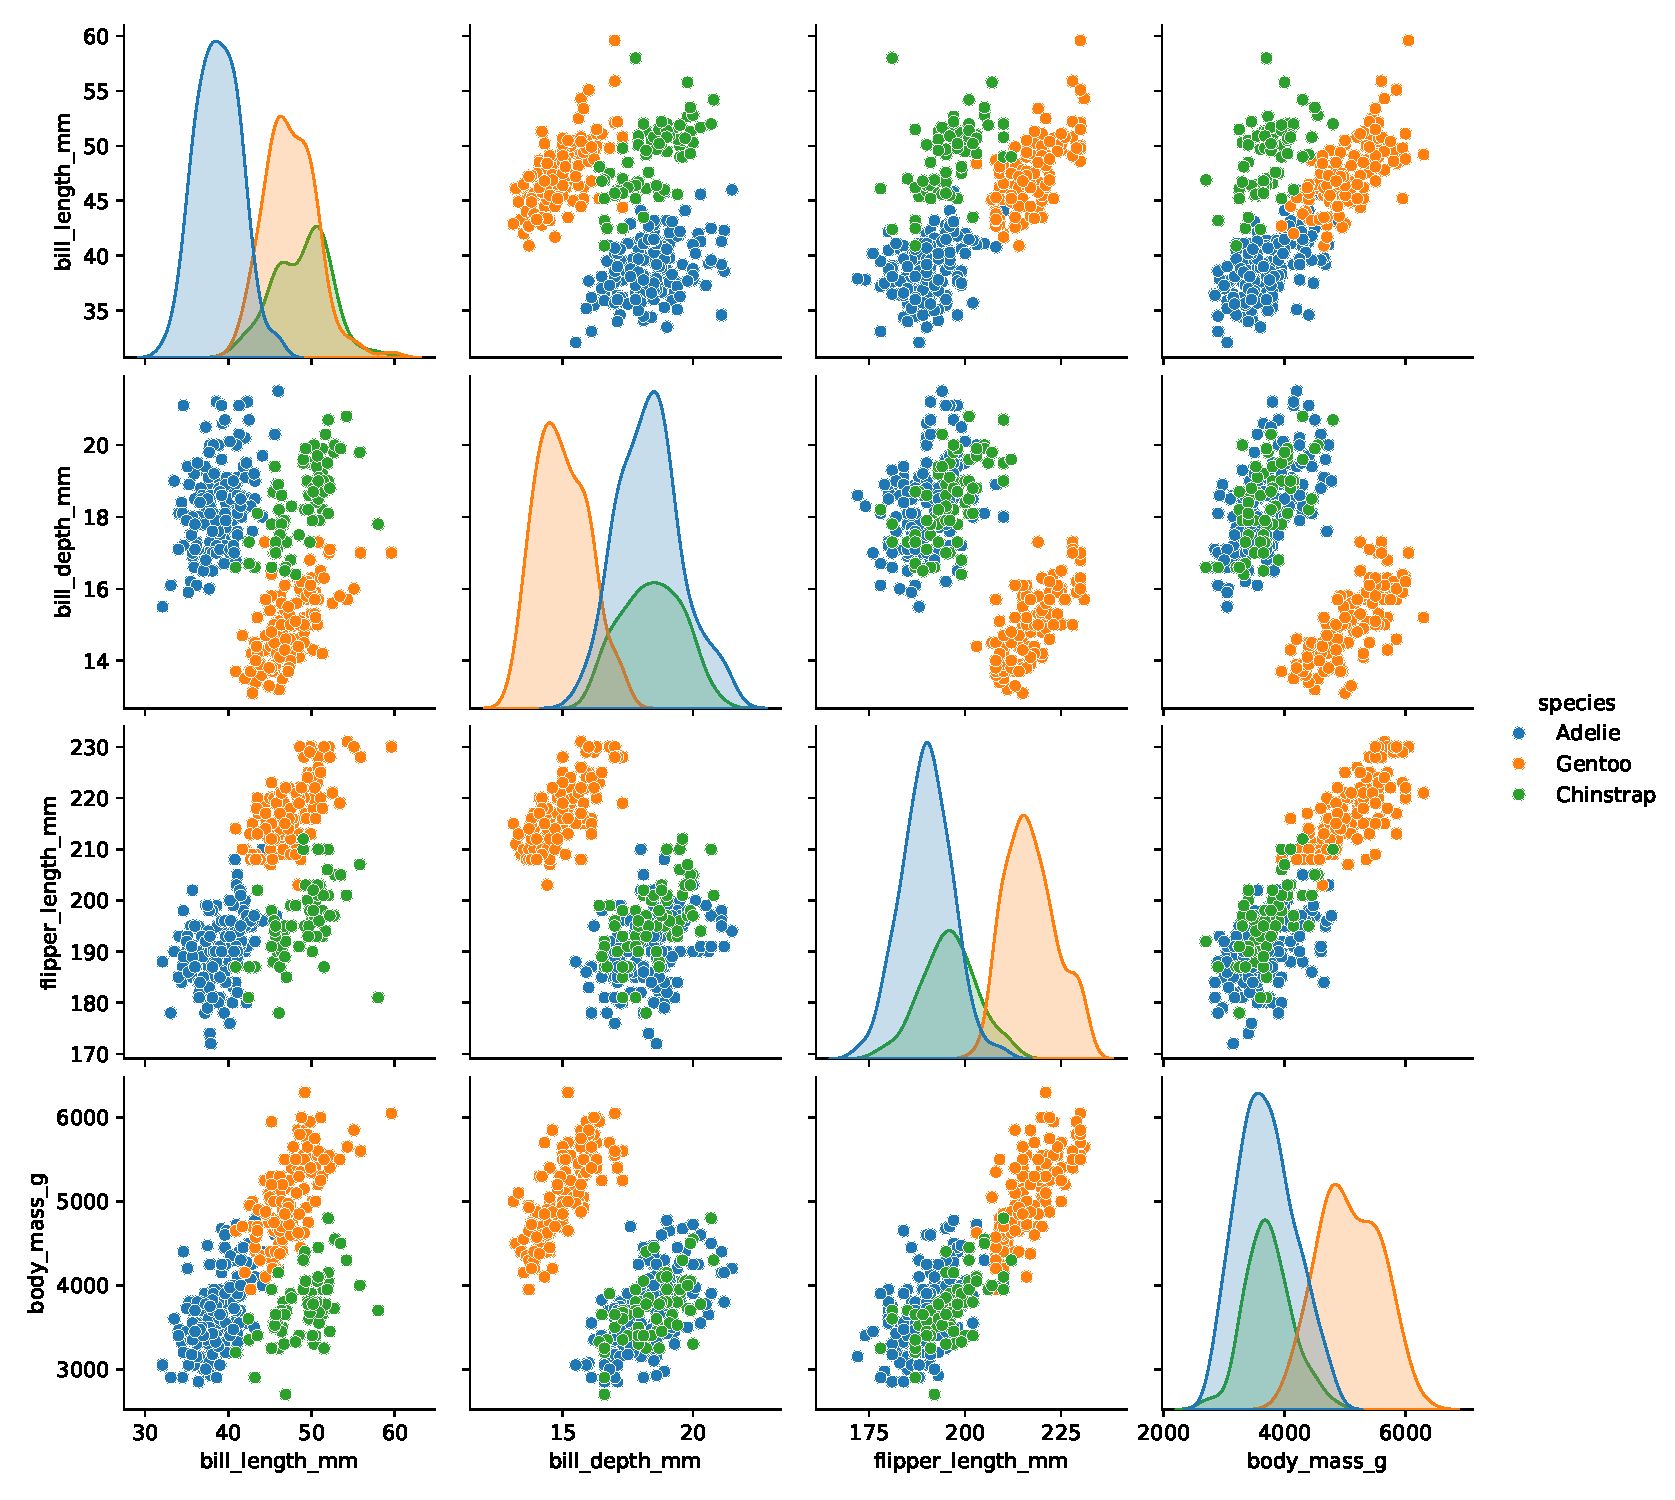
\includegraphics[width=15cm, height=13.5cm]{Penguins_scatterplot.pdf}
  \caption{Pairwise plots of the Penguin dataset for the bill length, bill depth, flipper length and body mass variables.}
  \label{fig:penguins_scatter}
\end{figure}

For this task, we will use the Python library UMAP \cite{mcinnes2018umap-software} to reduce the dimension in a way that preserves the topology of the 4-dimensional space we are working with. We can first remove the missing values and the columns we won't need for this short analysis. Since we are working with different scales, it is generally useful to convert the features into z-scores or use a different scaler process.

\begin{figure}[h!]
  \centering
  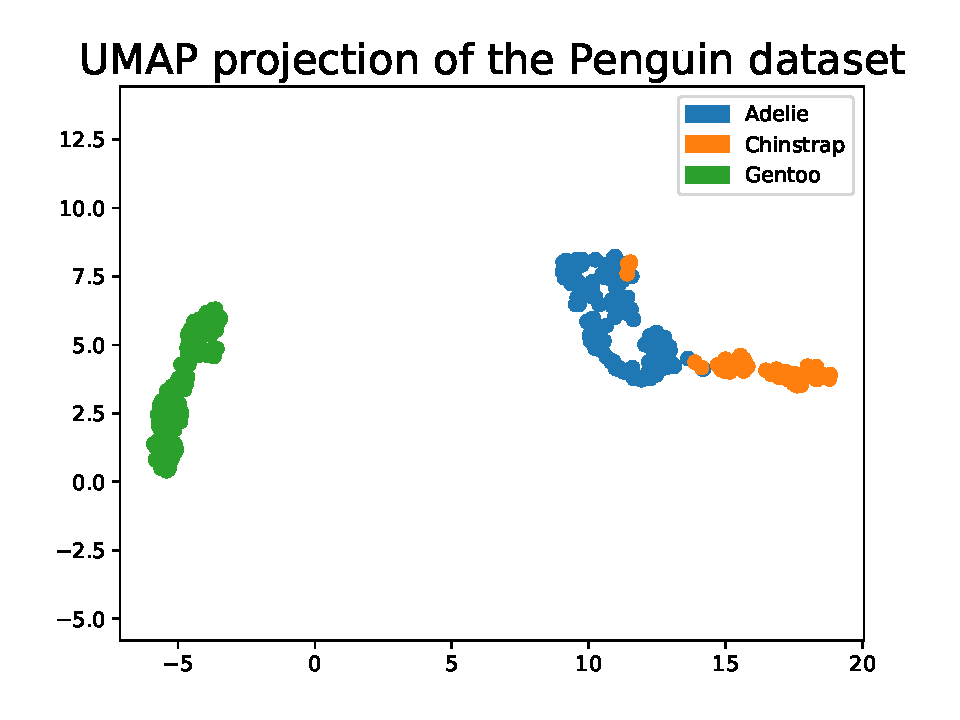
\includegraphics[width=12cm, height=10cm]{penguins_projection.pdf}
  \caption{UMAP dimension reduction result on the Penguin dataset.}
  \label{fig:penguins_projection}
\end{figure}

The result of reducing the dimension can be seen in \ref{fig:penguins_projection}. Comparing it to \ref{fig:penguins_scatter}, it does a good job of capturing the relationships between the three groups. Although, in this case specifically, we already found everything we needed in the scatter plot matrix, which was only possible because we worked with four dimensions. Once the number of features is higher, a scatter plot matrix becomes unwieldy and difficult to read properly.

\subsection{Digits dataset}
For an example with a high number of features, we can consider the known digits dataset \cite{optical_recognition_of_handwritten_digits_80}, one of the many toy datasets used to validate both old and new algorithms. We can iterate over the individual images to display them on a grid in \ref{fig:digits} to see what we are working with.

\begin{figure}[h!]
  \centering
  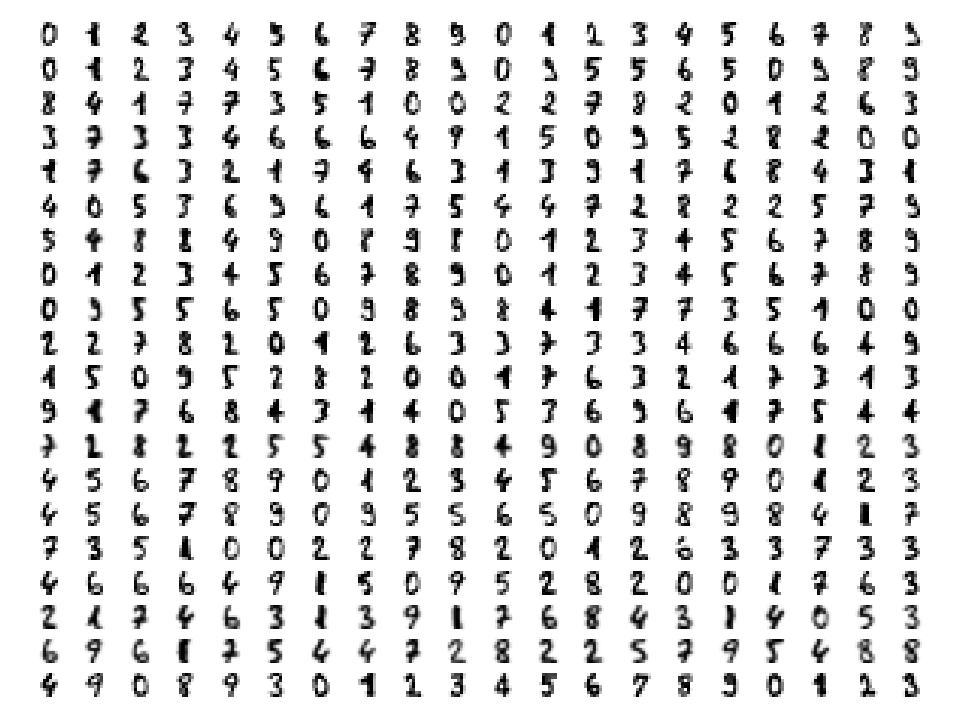
\includegraphics[width=12cm, height=10cm]{digits.pdf}
  \caption{First few images of the digits dataset}
  \label{fig:digits}
\end{figure}

The digits dataset contains 1797 bitmaps of hand-written digits in 10 classes -- each class corresponding to its digit. Most digits are somewhat readable but there are few that are simply too blurred to be considered useful for any further analysis. Such bitmaps should be separated into their own cluster of outliers, creating one additional class in the end.
The usual goal is to classify and cluster each bitmap into its appropriate class. We will see that with UMAP, we obtain satisfying results with a simple application of the algorithm. We see in \ref{fig:digits_projection} that reducing the dimension with UMAP already gave us a rather solid clustering of the digits with significant clusters. It shouldn't come off as a suprise that fairly distinct digits like 0, 9, 2, 6 or 7 are far away from the rest; whereas digits 1, 8, 3 lie close to each other.

\begin{figure}[h!]
  \centering
  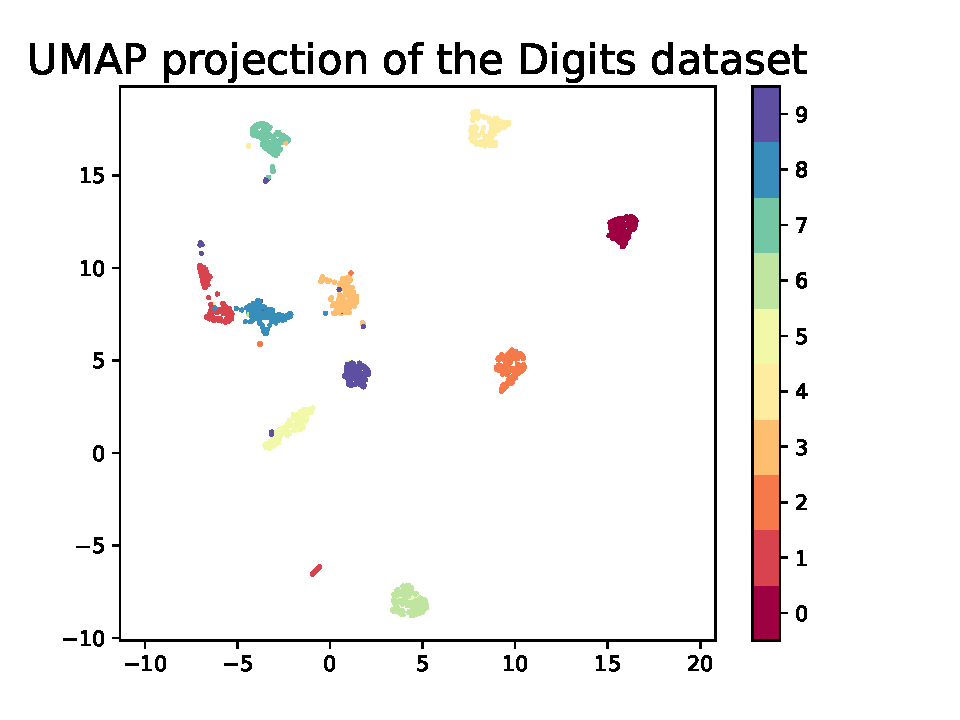
\includegraphics[width=12cm, height=11cm]{digits_projection.pdf}
  \caption{Result of UMAP on the digits dataset.}
  \label{fig:digits_projection}
\end{figure}

We will look into the digits dataset two more times -- once with Mapper in the next section and the second time using homology groups instead.

\subsection{Fashion and clothes}
We can look at a much larger dataset to see how UMAP compares. Fashion-MNIST \cite{DBLP:journals/corr/abs-1708-07747} is a dataset consisting of 60,000 examples of Zelando's clothing articles, each article being a 28x28 grayscale image associated to one of 10 classes. The classes go as follow, labelled from 0 to 9 -- T-shirt, Trouser, Pullover, Dress, Coat, Sandal, Shirt, Sneaker, Bag, and Ankle Boot.
As was the case for the digits dataset, one is typically interested in classifying and clustering the clothing articles while removing the images that are too blurred. Applying UMAP, we can see the resulting projection on \ref{fig:fmnist}. On a more technical note, the MNIST dataset should be ideally replaced with a different one since it is too easy for modern machine learning algorithms, is usually overused and cannot represent modern Computer Vision tasks. But since this text isn't about Computer Vision, we can safely proceed.

\begin{figure}[h!]
  \centering
  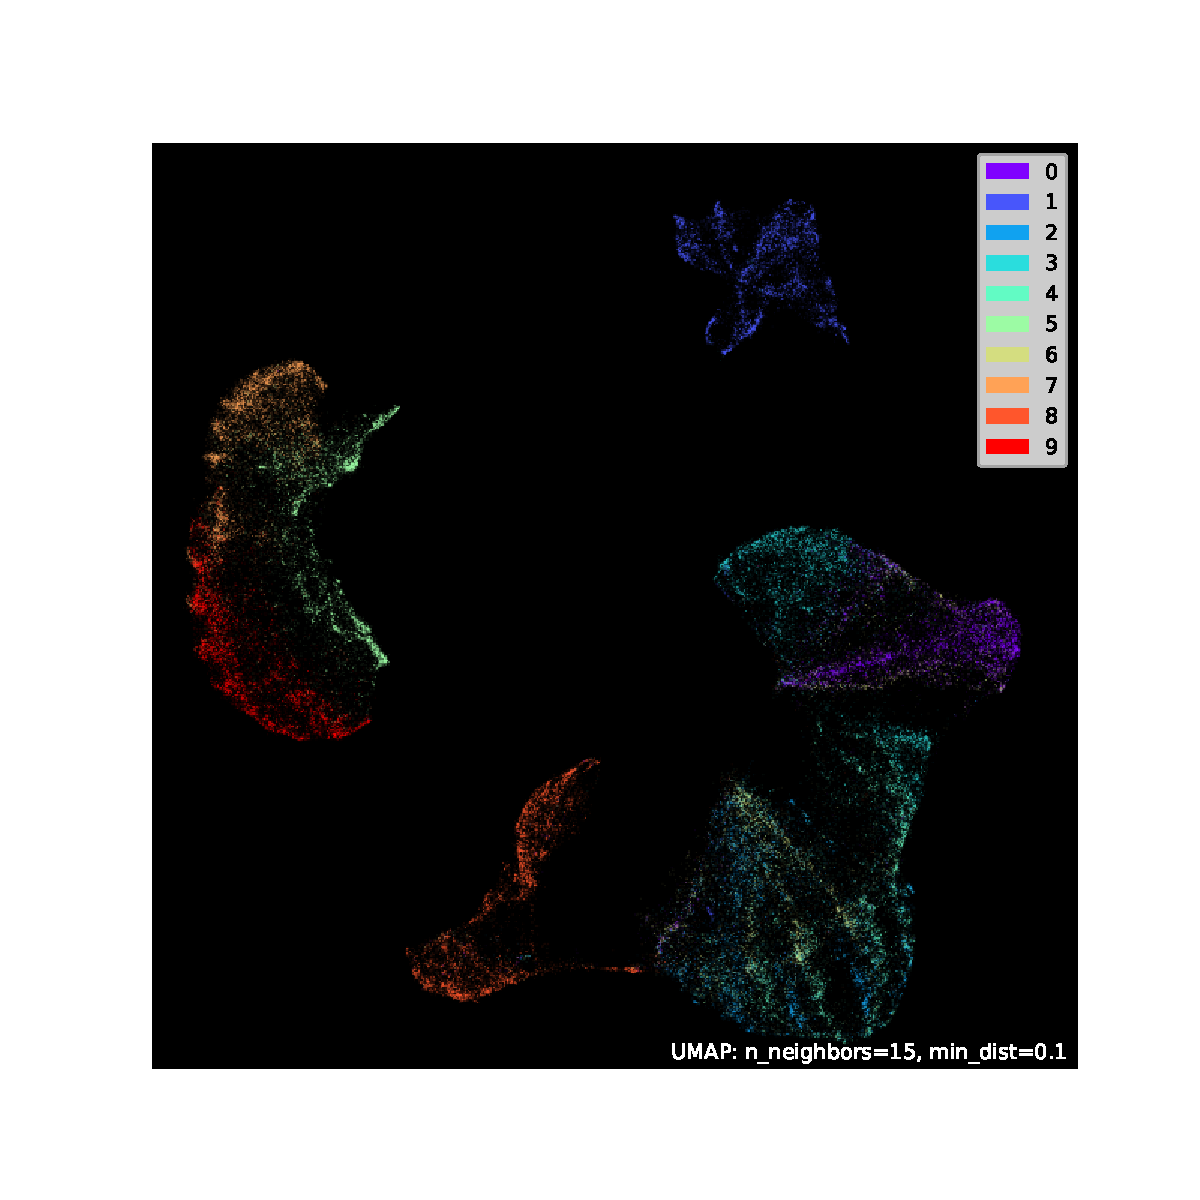
\includegraphics[width=12cm, height=10cm]{fmnist.pdf}
  \caption{Result of UMAP on the much larger Fashion-MNIST dataset.}
  \label{fig:fmnist}
\end{figure}

It intuitively makes sense to see that shoes should be generally projected close to each other, as we see with sneakers, sandals and ankle boots. Trousers are found in the top-left corner, isolated from the rest. In the \textit{UMAP examples} notebook, we also provide an interactive version of the resulting projection on a subset of Fashion-MNIST, allowing the user to see the labels of individual points upon zooming.

An interesting property that UMAP allows us to study is the connectivity of the topological representation of the original high-dimensional data. This can be useful for diagnostic purposes, but in the case of this text, it corresponds to studying the connected components. It should be noted that computing and plotting the connectivity of the dataset can be rather expensive, so it is recommended to check subsamples instead. We can see examples of it on \ref{fig:fmnist_connectivity} and \ref{fig:fmnist_connectivity_hammer}.

\begin{figure}[h!]
  \centering
  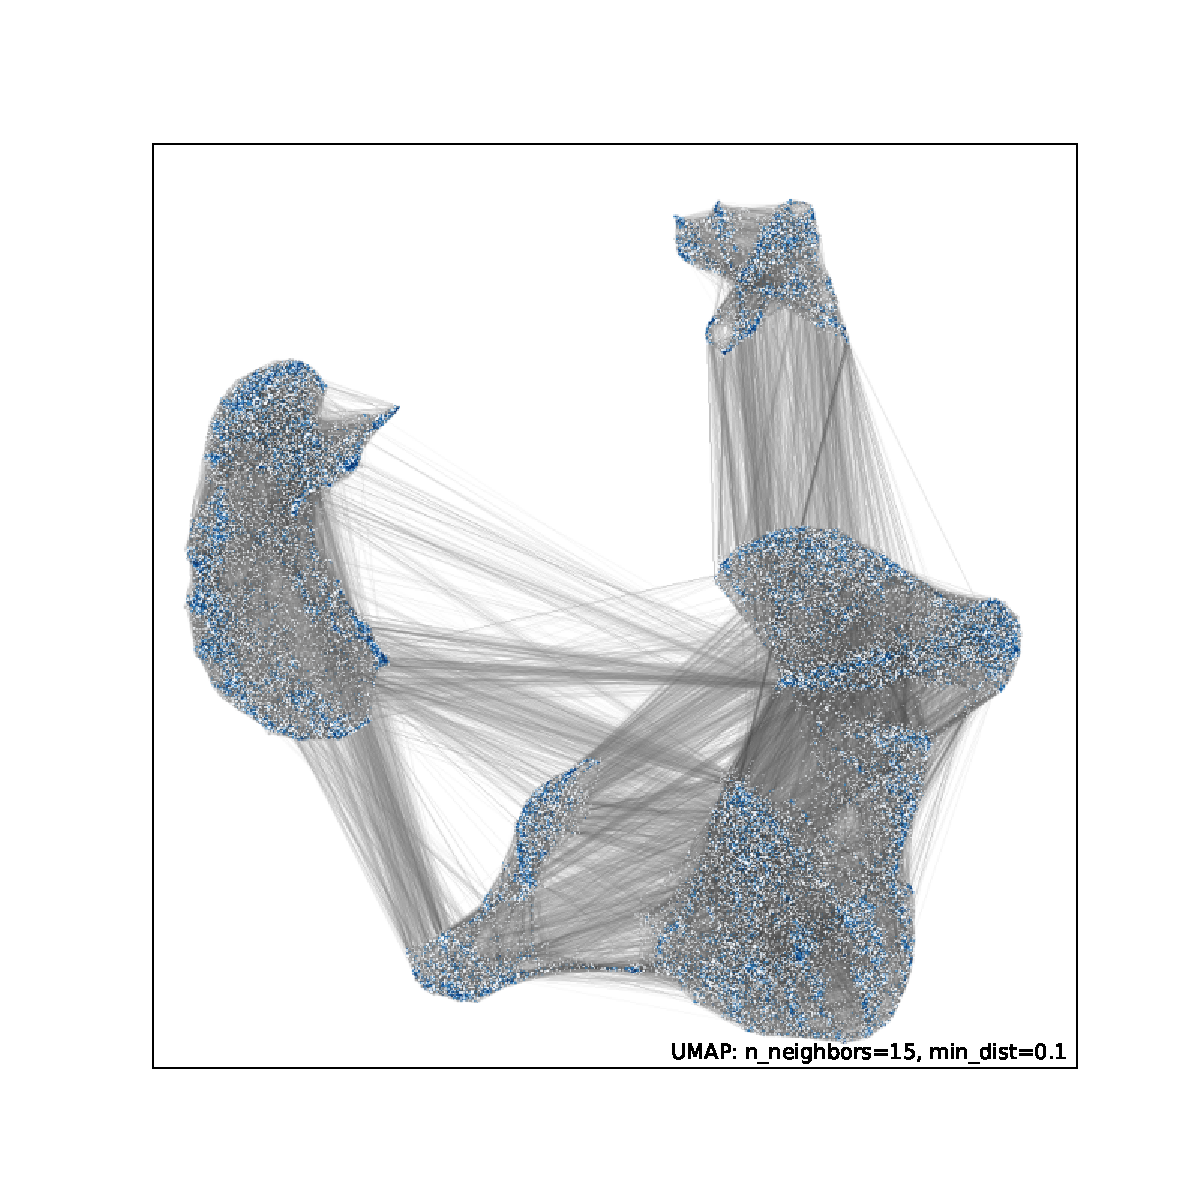
\includegraphics[width=12cm, height=10cm]{fmnist_connectivity.pdf}
  \caption{Points of connectivity of Fashion-MNIST.}
  \label{fig:fmnist_connectivity}
\end{figure}

\begin{figure}[h!]
  \centering
  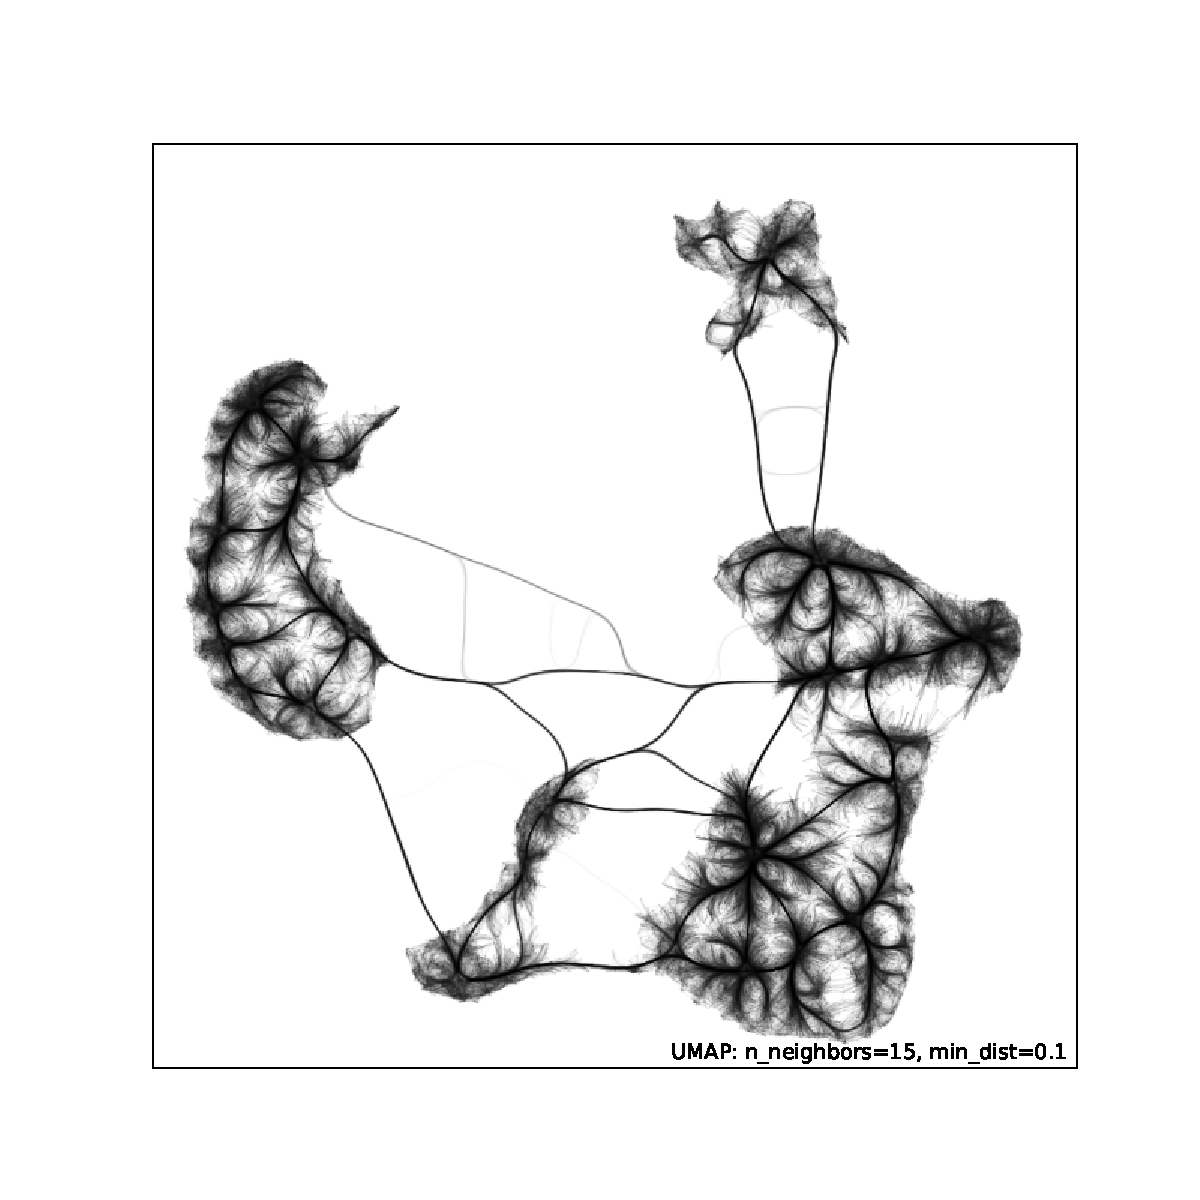
\includegraphics[width=12cm, height=10cm]{fmnist_connectivity_hammer.pdf}
  \caption{A less busy view of connectivity of Fashion-MNIST.}
  \label{fig:fmnist_connectivity_hammer}
\end{figure}

\section{Mapper}
As was mentioned in the beginning of this text, the methods of persistence topology can become computationally infeasible for larger datasets, making them practically unusable for datasets with measurements in the counts of millions and above. This was seen in the rapidly-growing number of simplices in the Vietoris-Rips complex. Furthermore, interpreting the output of persistence homology for high-dimensional data can be difficult to interpret (what does the presence of a 1-dimensional loop in a 50-dimensional space indicate?). One approach to tackle this issue is to combine persistence with clustering, resulting in the Mapper algorithm that we're going to discuss.

We're going to introduce the multiscale clustering method of Singh, Mémoli and Carlsson \cite{singh2007topological}. Let's assume that the data is presented as a finite metric space $(P, d)$. Let us then choose:

\begin{itemize}
  \item a \textit{filter function} $f: P \to \mathbb{R}^{n}$
  \item a cover $\mathcal{C} = \{U_{\alpha}\}$ of the range of $f$ in $\mathbb{R}^{n}$
\end{itemize}
The cover is typically taken to be a collection of overlapping cubes. In $\mathbb{R}$, we would be looking at a collection of closed intervals. Software packages will want you to specify the number of covering intervals and the percentage of overlap you allow. We then proceed with the algorithms as follows:

\begin{enumerate}
  \item Cluster each inverse image $f^{-1}(U_{\alpha}) \subseteq P$, regarded as a metric subspace of $P$, for all $U_{\alpha} \in \mathcal{C}$. Denote by $C_{\alpha, i}$ the i-th cluster. Here, a point can appear in multiple nodes due to the overlap.

  \item Form a graph where the vertices are given by the clusters $C_{\alpha, i}$ as $\alpha$ and $i$ vary and there is an edge between $C_{\alpha, i}$ and $C_{\alpha', j}$ when
        \begin{equation*}
          C_{\alpha, i} \cap C_{\alpha', j} \neq \varnothing
        \end{equation*}

  \item Assign a color to each vertex in the graph corresponding to a particular cluster $C_{\alpha, i}$ according to the average value of $f$ on $x \in C_{\alpha, i}$.
\end{enumerate}

Mapper's strength lies in the flexibility of choices we can make during the creation of the graph. For the projection, we can take any projection method from mathematics, statistics, machine learning or  econometrics -- PCA, t-SNE, UMAP, even something as simple as projecting on the $x-$axis.

The same applies for the choice of clustering algorithms. We can pick any method -- hierarchical, density-based and any distance metric. The distance metric does not need to satisfy the triangle inequality, giving us the option to choose from the wider range of similarity metrics like the Kullback-Leibler divergence and so on.

Because Mapper is primarily a visual tool, most software packages include additional tooling to improve upon the basic algorithm and help with further exploration. That may involve a combination of the following:

\begin{itemize}
  \item Size the nodes by a function of interest (number of members inside the cluster, etc.)
  \item Color the nodes by a function of interest (average spendings, number of purchases, etc.)
  \item Shape the nodes given some condition (circles for group 1, squares for group 2, etc.)
  \item Size the graph edges by a function of interest (number of overlapping cluster members, etc.)
  \item Color the graph edges by a function of interest (average color of connected nodes, etc.)
  \item Shape the graph edges given a condition (dotted lines for group 1, solid line elsewhere, etc.)
  \item Descriptive statistics on the nodes and the graph
\end{itemize}

All in all, this makes Mapper one of the most flexible approaches to dataset visualizations, giving the user the option the construct the final graph exactly the way they intended. For the Mapper examples, we will make use of the Python libraries \textit{scikit-tda} \cite{scikittda2019} and \textit{giotto-tda} \cite{tauzin2020giottotda}.

We can start with simple, synthetic examples before moving onto real data to see what the results of Mapper are and how they differ when we change the parameters or used methods.

\subsection{Toy examples}
We will start by generating 5000 points sampled from two nested circles in the plane with some added Gaussian noise. We can see the plotted dataset in \ref{fig:mapper_circles}. In our first attempt, we will project our data onto the $x-$ and $y-$axes, choose 10 covering intervals with a 30\% overlap and use the DBSCAN clustering algorithm.

In figure \ref{fig:mapper_circles_graph} we can see that Mapper succesfuly captured the salient features - those being the two holes in the nested circles. The coloring of the node used the default settings of \textit{giotto-tda} -- coloring the nodes by the average row index of the data in the cluster; with 5000 generated points, we thus have 5000 rows. The node size here is given by the number of data points in the node.

\begin{figure}[h!]
  \centering
  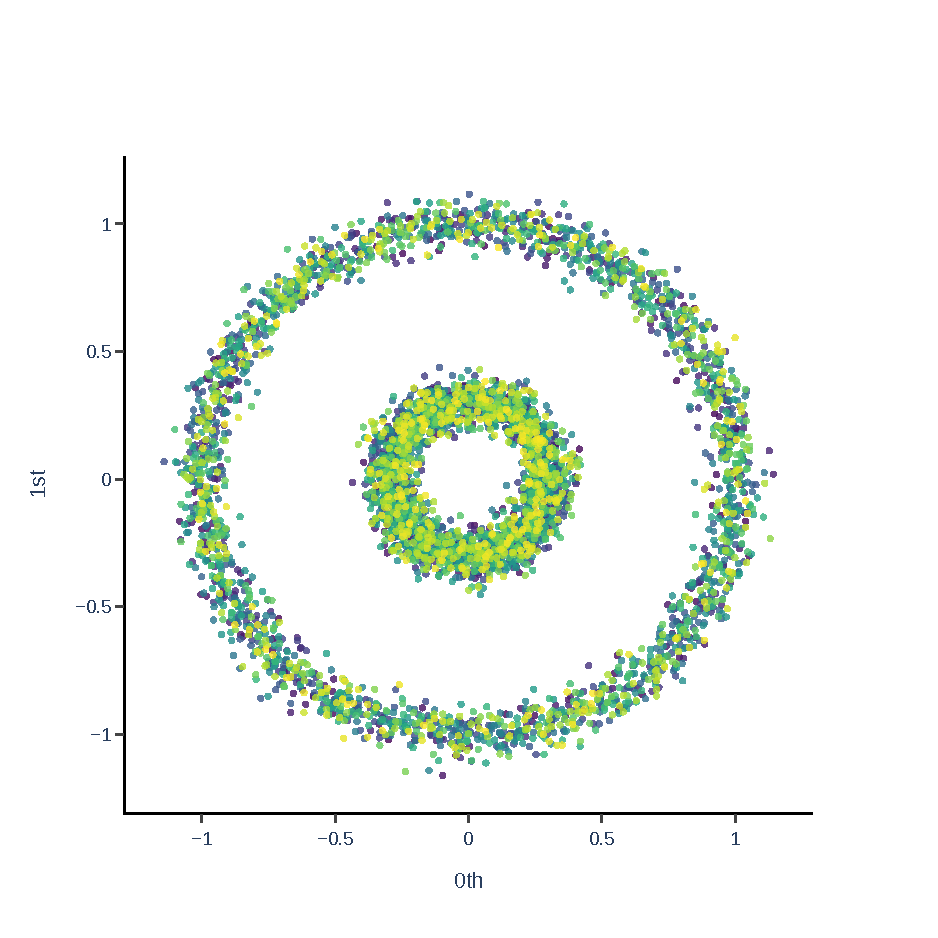
\includegraphics[width=10cm, height=10cm]{mapper_circles.pdf}
  \caption{Our toy example for now - two nested circles.}
  \label{fig:mapper_circles}
\end{figure}

\begin{figure}[h!]
  \centering
  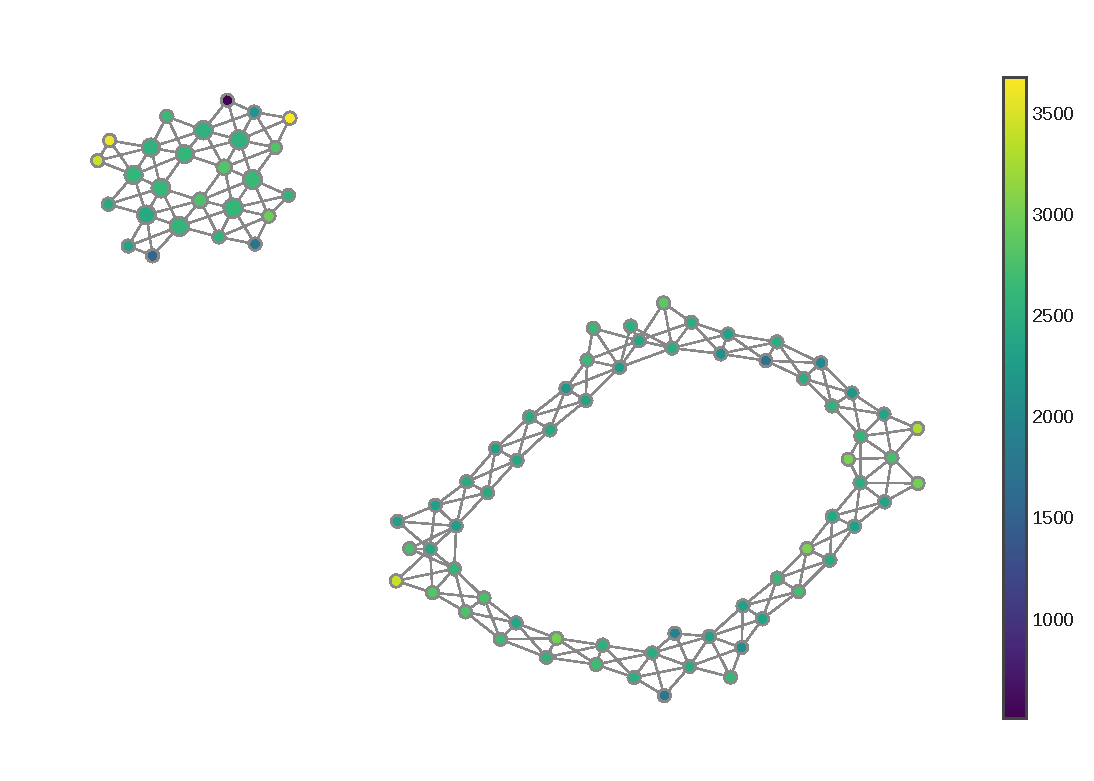
\includegraphics[width=10cm, height=10cm]{mapper_circles_graph.pdf}
  \caption{First result of applying Mapper.}
  \label{fig:mapper_circles_graph}
\end{figure}

The coloring or the size do not convey any particularly interesting information in this case; here we were more interested to recover the presence of the two underlying holes. On the other hand, coloring by the average value of the $x-$ or $y-$coordinates would be more instructive, as revealed on \ref{fig:mapper_circles_coordinates}. Here we see that the $x-$coordinates of the inner circle, closer to the origin, are colored in such a way that lies near the $0$ point of the spectrum. We would see a similar, but flipped, version of the coloring had we used the $y$-coordinates instead.

\begin{figure}[h!]
  \centering
  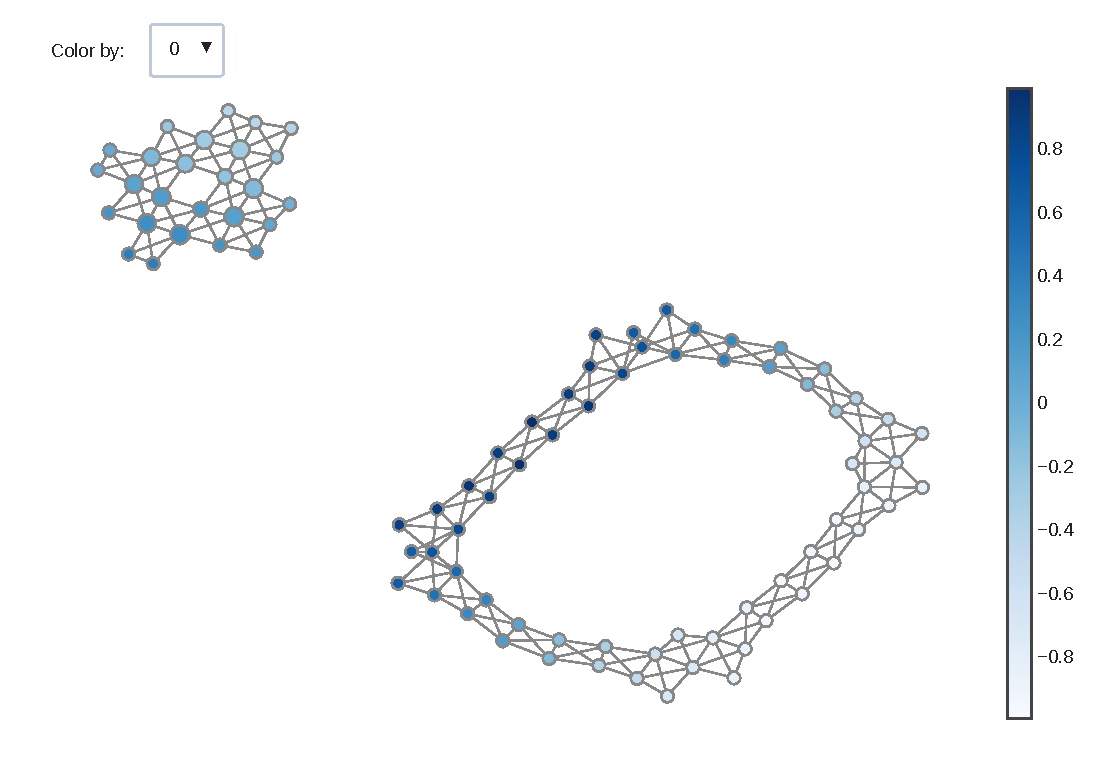
\includegraphics[width=10cm, height=10cm]{mapper_circles_coordinates.pdf}
  \caption{Nodes colored by the average $x$-coordinate.}
  \label{fig:mapper_circles_coordinates}
\end{figure}

We can, if we want to, color by something like the first principal component of PCA, as seen in \ref{fig:mapper_circles_pca}. In this context, it doesn't reveal anything particularly interesting but it may be more useful in applications where PCA is actively used.

\begin{figure}[h!]
  \centering
  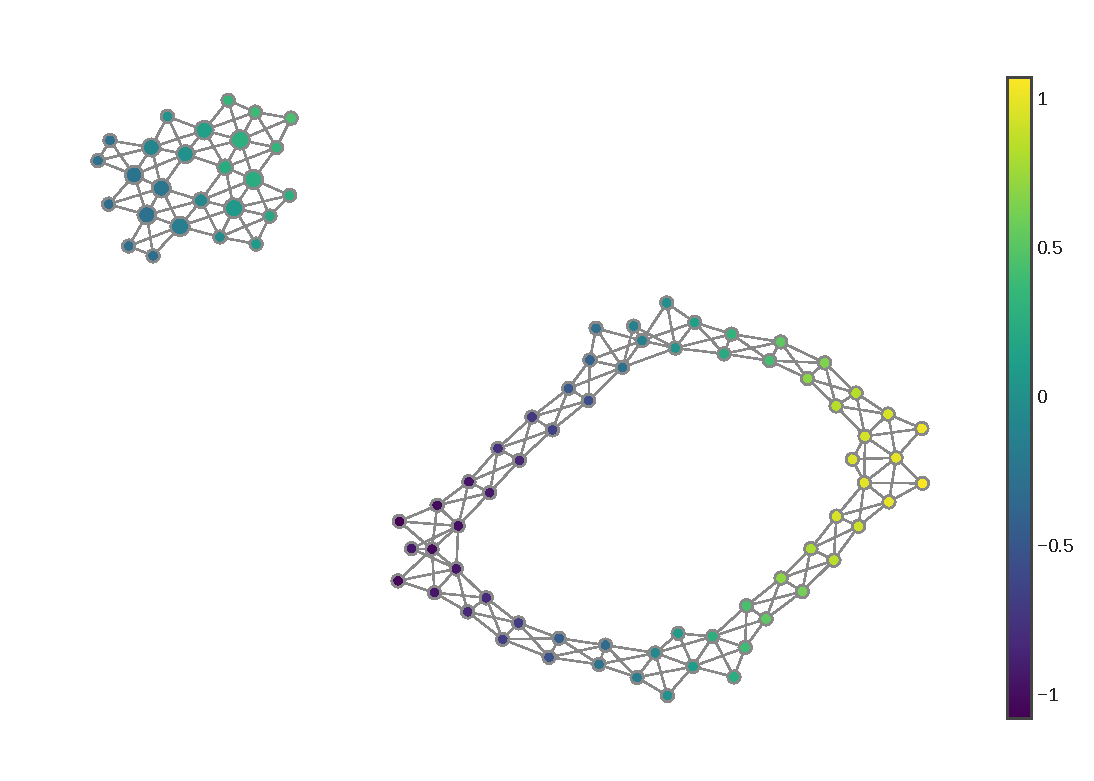
\includegraphics[width=10cm, height=10cm]{mapper_circles_pca.pdf}
  \caption{Nodes colored by the average first PCA component.}
  \label{fig:mapper_circles_pca}
\end{figure}

As mentioned above, we can colord by proportions of some categorical variable -- one that is either already present or one that we create. Let us try to separate the inner and outer circle more cleanly. We can add a categorical column to the dataframe, with a value of ``A'' for the outer circle and ``B'' for the inner circle, where the testing criterium is whether
\begin{equation*}
  x^{2} + y^{2} < \frac{1}{4}.
\end{equation*}

The result of this can be seen on \ref{fig:mapper_circles_groups}, where the inner and outer circle are now exactly separated. As with the coordinates, we would see a flipped version of this graph for group ``B''. It should also be noted that the color spectrum only attains two values -- $\{0, 1\}$.

\begin{figure}[h!]
  \centering
  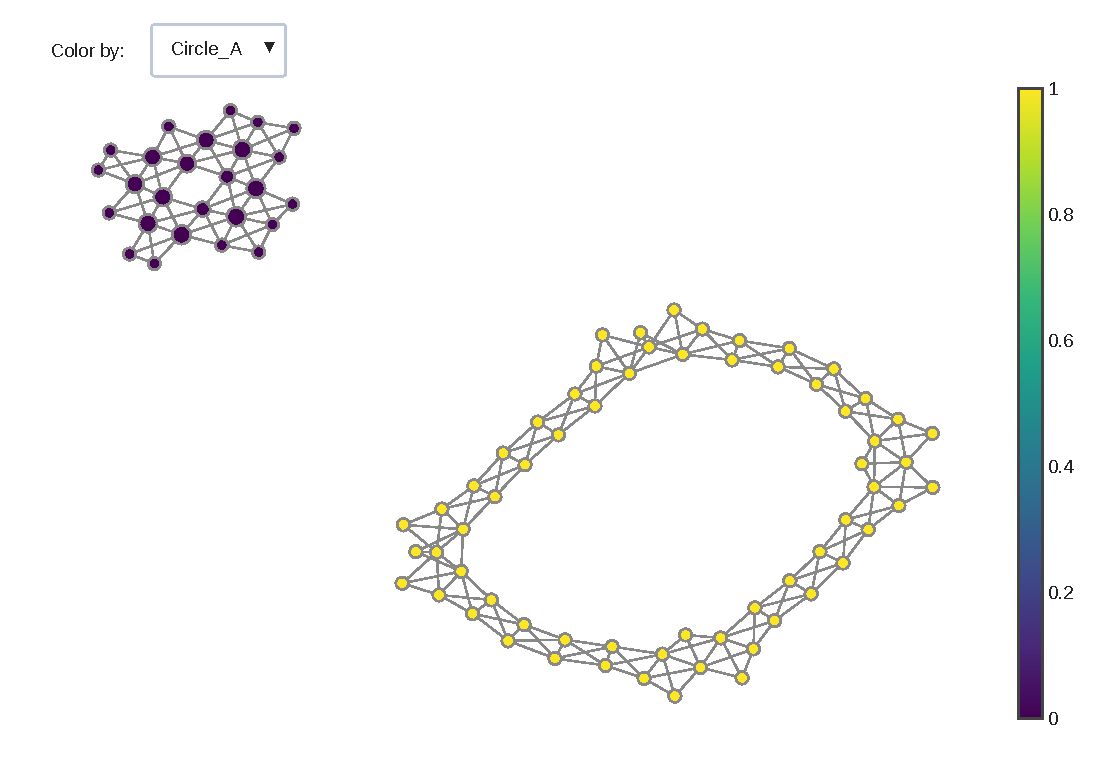
\includegraphics[width=10cm, height=10cm]{mapper_circles_groups.pdf}
  \caption{Nodes colored by categorical variables.}
  \label{fig:mapper_circles_groups}
\end{figure}

Finally, we can take a look and compare what happens when we use a different filtration function on the dataset. For example, we could project by taking the sum of the $(x,y)$ coordinates. This results in \ref{fig:mapper_circles_sum}.

\begin{figure}[h!]
  \centering
  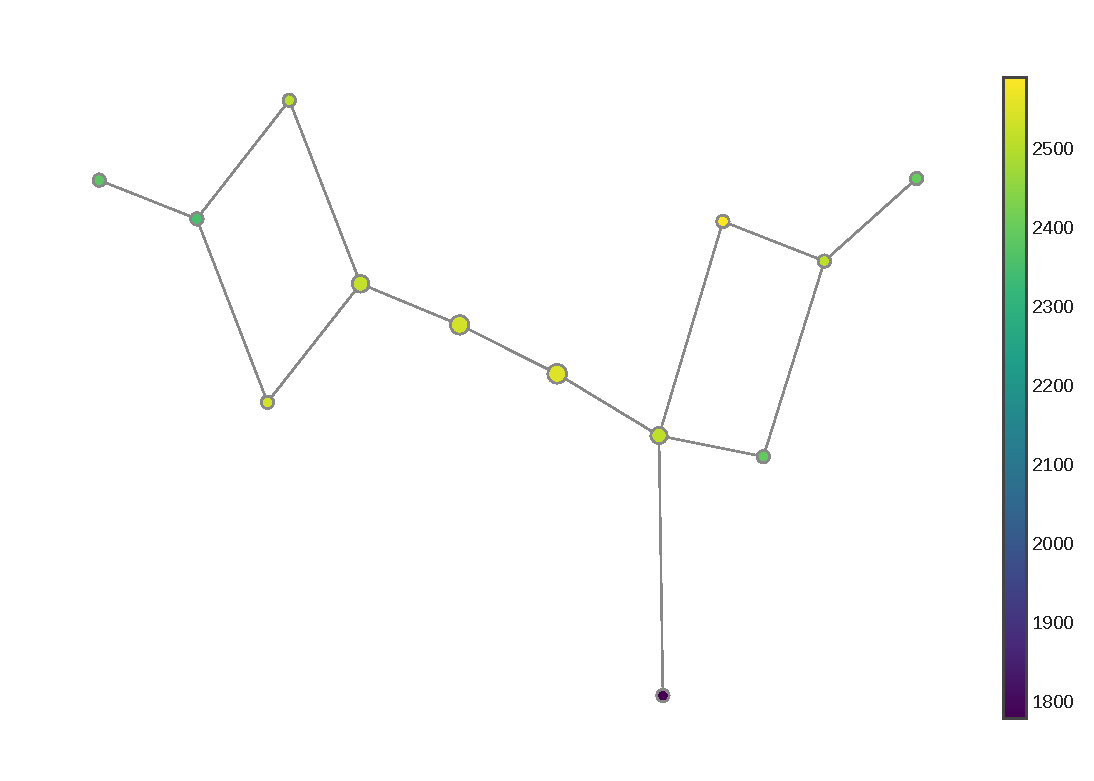
\includegraphics[width=12cm, height=10cm]{mapper_circles_sum.pdf}
  \caption{The effect of a different filtration function; in this case, the sum of the individual coordinates.}
  \label{fig:mapper_circles_sum}
\end{figure}

The presence of the two loops was still properly encoded, although this time we don't have the same level of separation as we did by projecting on the individual coordinates.

\subsection{Stock market data}
We can now take a look at how one could potentially use Mapper to improve your analysis of stock market data. Specifically, we will look at the closing prices of the SP500 index companies, starting from 01.01.2024 up to 01.01.2025. The choice of date is arbitrary, and one could easily choose a much larger time interval to consider, but for the sake of this example, one year will suffice. The data was fetched from Yahoo Finance through their API and stored in a data frame. A simple indicator of interest when dealing with stock market data is the log-return of the stock price. As such, our first filtration function will be the log-percent return after the data is normalized.

Our goal here will be to cluster the company tickers in a way that similar behaviour of the stock value is represented in similar tickers sharing the same cluster. We could take the transpose of our dataset instead and try to cluster the 252 trading days of the year. This could perhaps be useful if we wanted to analyze which days or periods of the year showed significant drops or increases in the SP500 index. We could then correlate the clusters with geopolitical events such as the US presidential election, which brought an increase in stock prices for large tech companies, for example.

After normalizing the dataset, we first reduced the dimension to 150 via the Isomap algorithm before using UMAP to reduce it to 2. Our clustering algorithm of choice here was DBSCAN with the cosine metric. Using \textit{scikit-tda}, the result is stored in a \textit{html} file that you can open in your web browser. All the files for this section can be located in the \textit{figures/} folder. Our first view can be seen on \ref{fig:mapper_log_return}.

\begin{figure}[h!]
  \centering
  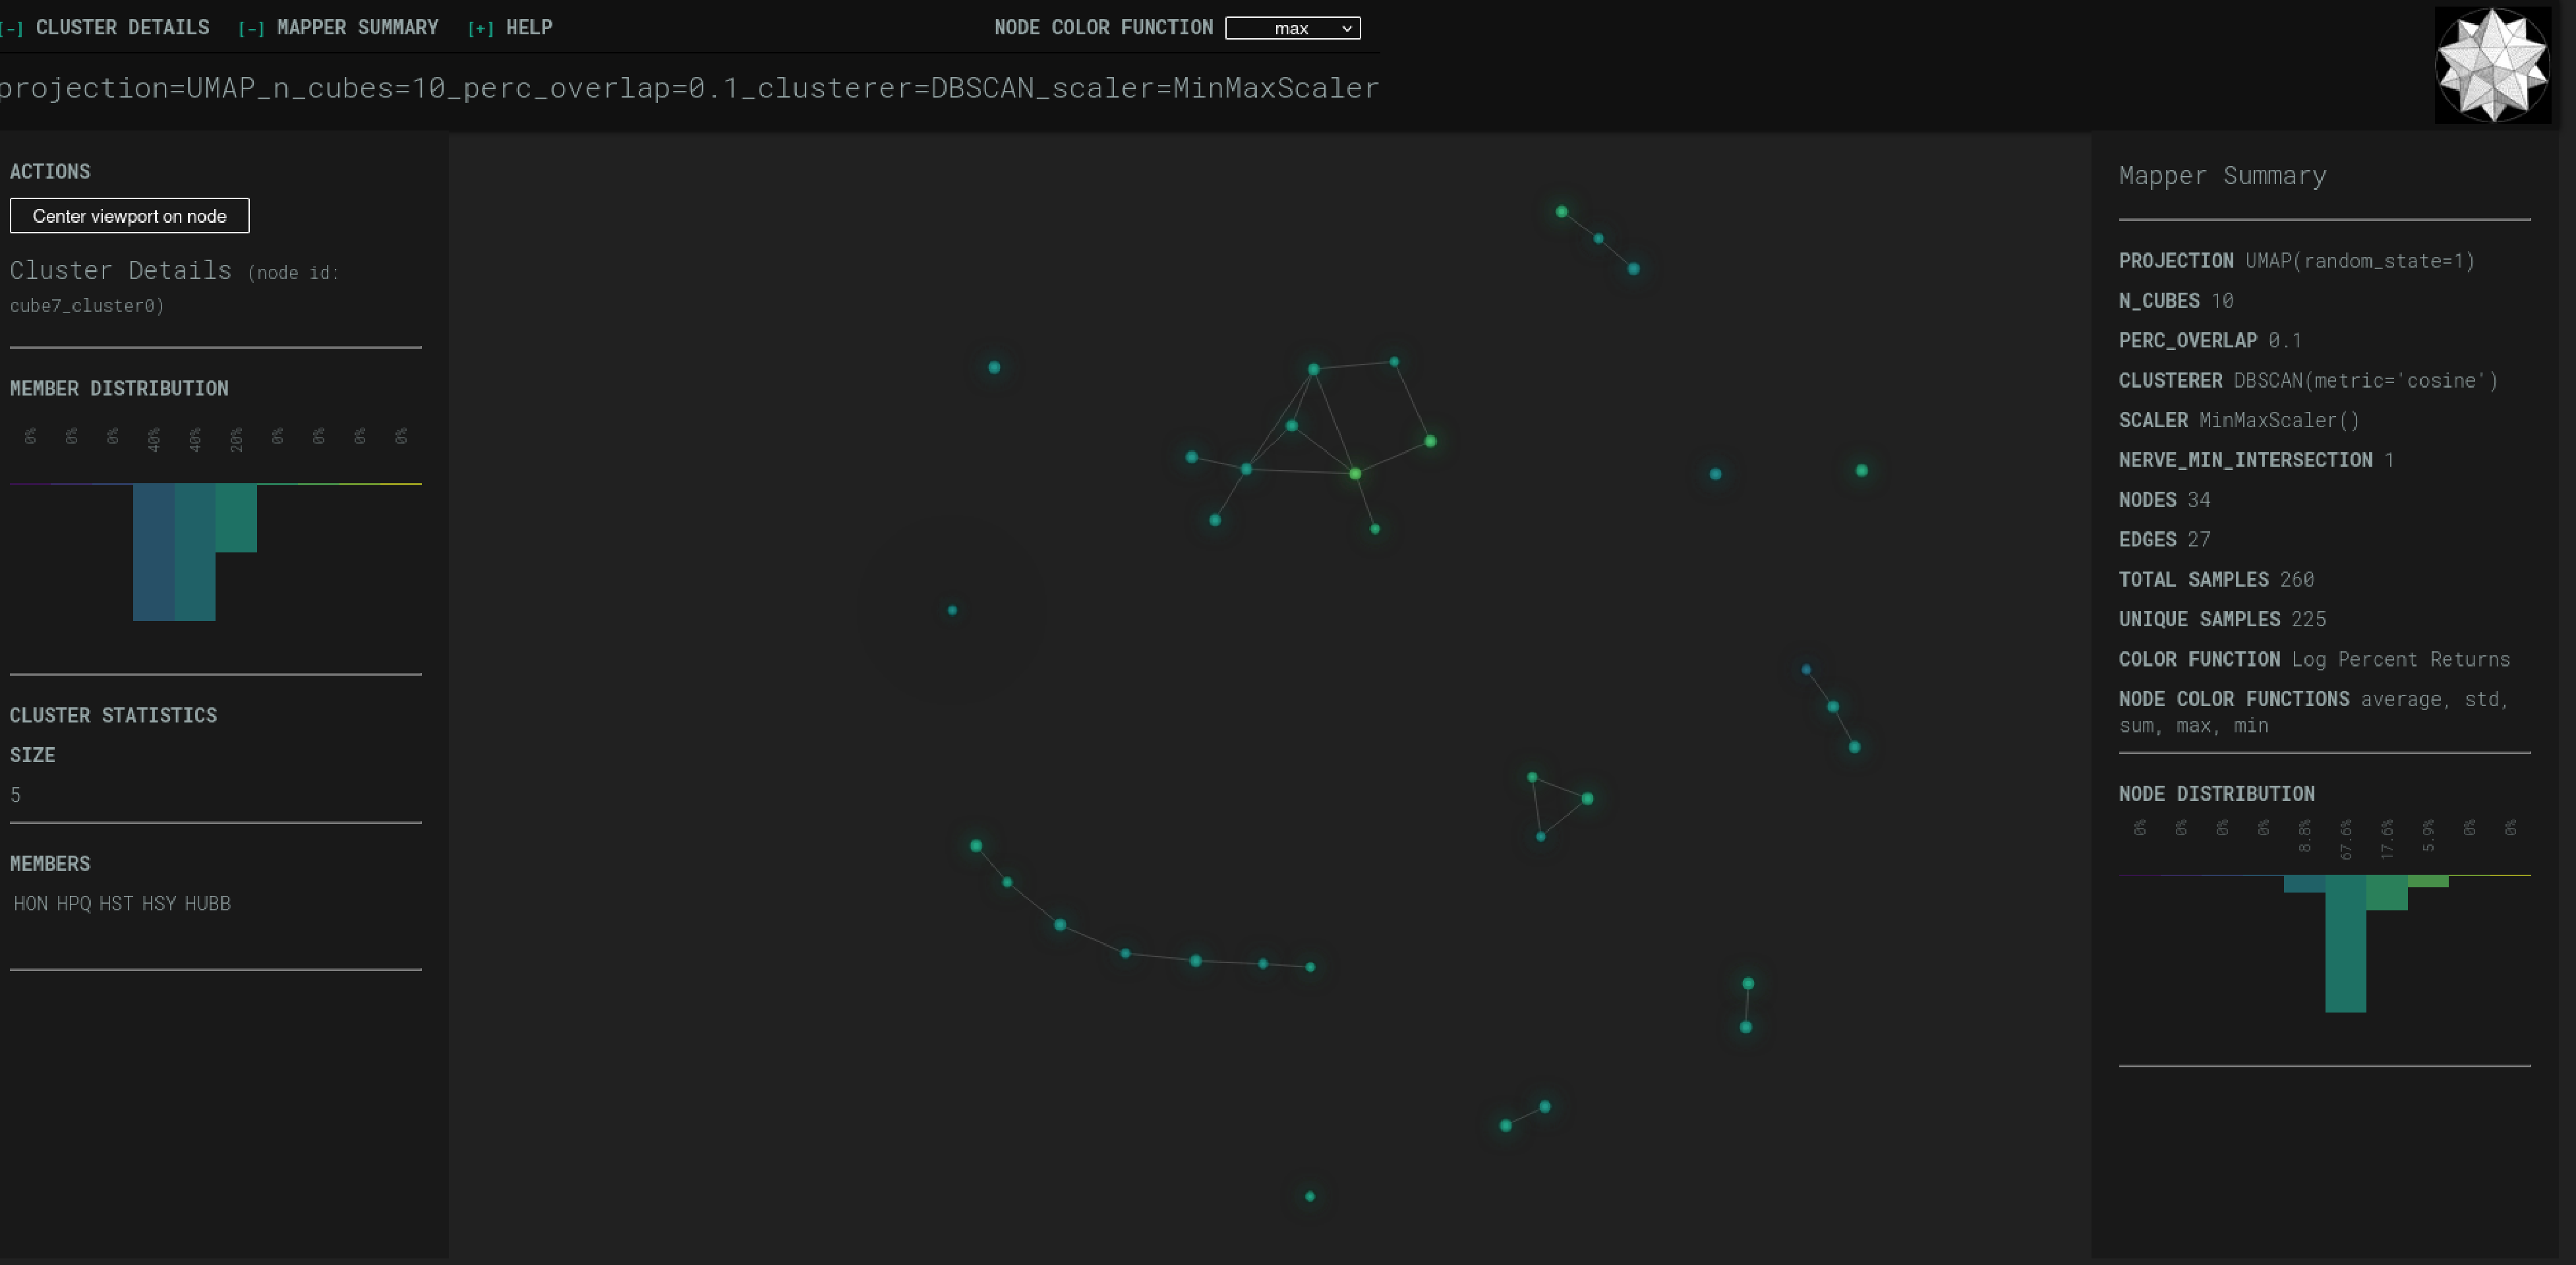
\includegraphics[width=15cm, height=12cm]{Mapper_log_return_example.pdf}
  \caption{View of the Mapper clustering summary with \textit{scikit-tda}.}
  \label{fig:mapper_log_return}
\end{figure}

We interpret the results as follows -- given that our color function is the log-percent return of the individual tickers, the clusters correspond to tickers who share a similar trading profile between each other. That is, underperformers would have darker colors, while companies that performed exceptionally well would be on the brighter end of the spectrum. In the graph \ref{fig:mapper_log_return}, we added multiple cluster coloring rules to compare. As mentioned previously, the default strategy is to color the final cluster by the average of the nodes inside. Here, we can also color by the average, maximum, minimum, the sum or the standard deviation. The only interesting results are when we look at the minimum and maximum log-percent returns of the clusters. While we have some stocks that performed better than the rest, most companies had a similar run during that one year. One could anticipate greater differences had we considered the closing prices over multiple years instead.

We could also choose a different color function, such as the volatility of the underlying stock. The notion of volatility we will look at is quite crude -- we simply take the standard deviation of the stock prices over the 252 days. Stock traders and market specialists would throttle us for this gross simplification, which is why we ignore their opinions and continue. The different color function drastically changes the resulting graph, as seen in \ref{fig:mapper_volatility}.

\begin{figure}[h!]
  \centering
  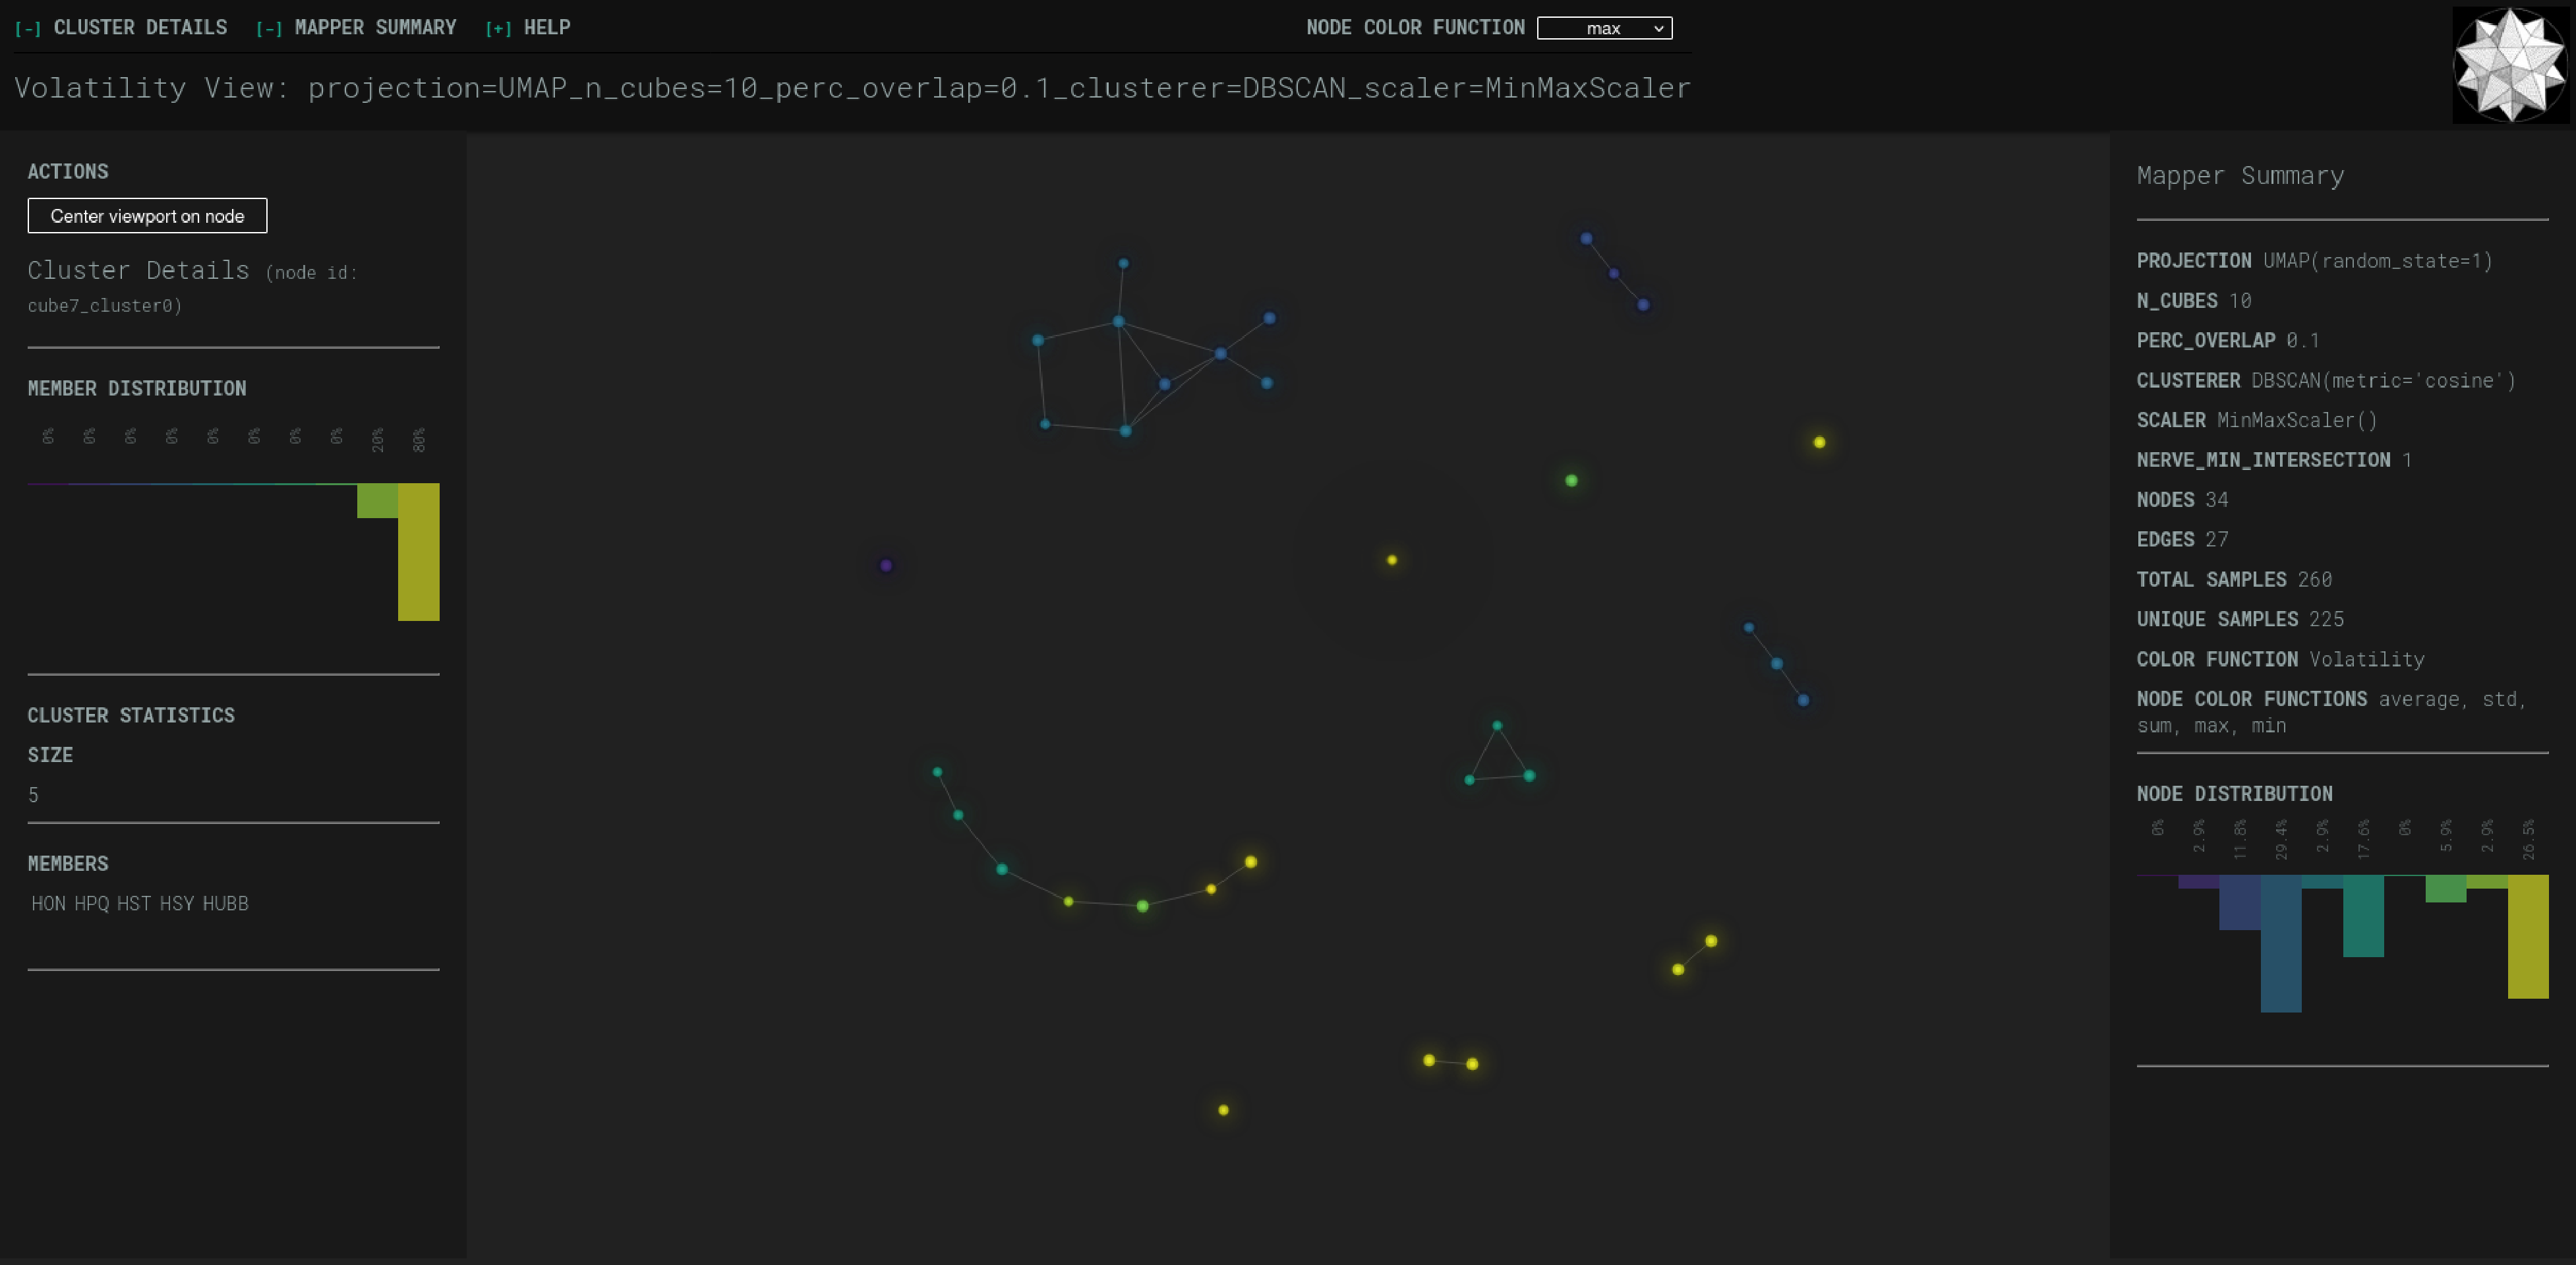
\includegraphics[width=15cm, height=12cm]{Mapper_volatility.pdf}
  \caption{Mapper graph of the SP500 data with the color function being the volatility of the stock.}
  \label{fig:mapper_volatility}
\end{figure}

Here we use the maximum of the volatility to color the resulting clusters, looking for stocks with an unusually high variance in the closing prices. Already, we can see that we have more outliers on both ends of the color spectrum, compared to the log-percent return. The benefit of the Mapper implementation in \textit{scikit-tda} is that it allows us to see directly which SP500 tickers are in the clusters by simply hovering over them. It also gives us the cluster ID, allowing us to plot the cluster data separatly from the rest. This way, we can plot the dark purple cluster, suggesting the lowest maximal volatility of closing prices in \ref{fig:mapper_volatility_low}.

\begin{figure}[h!]
  \centering
  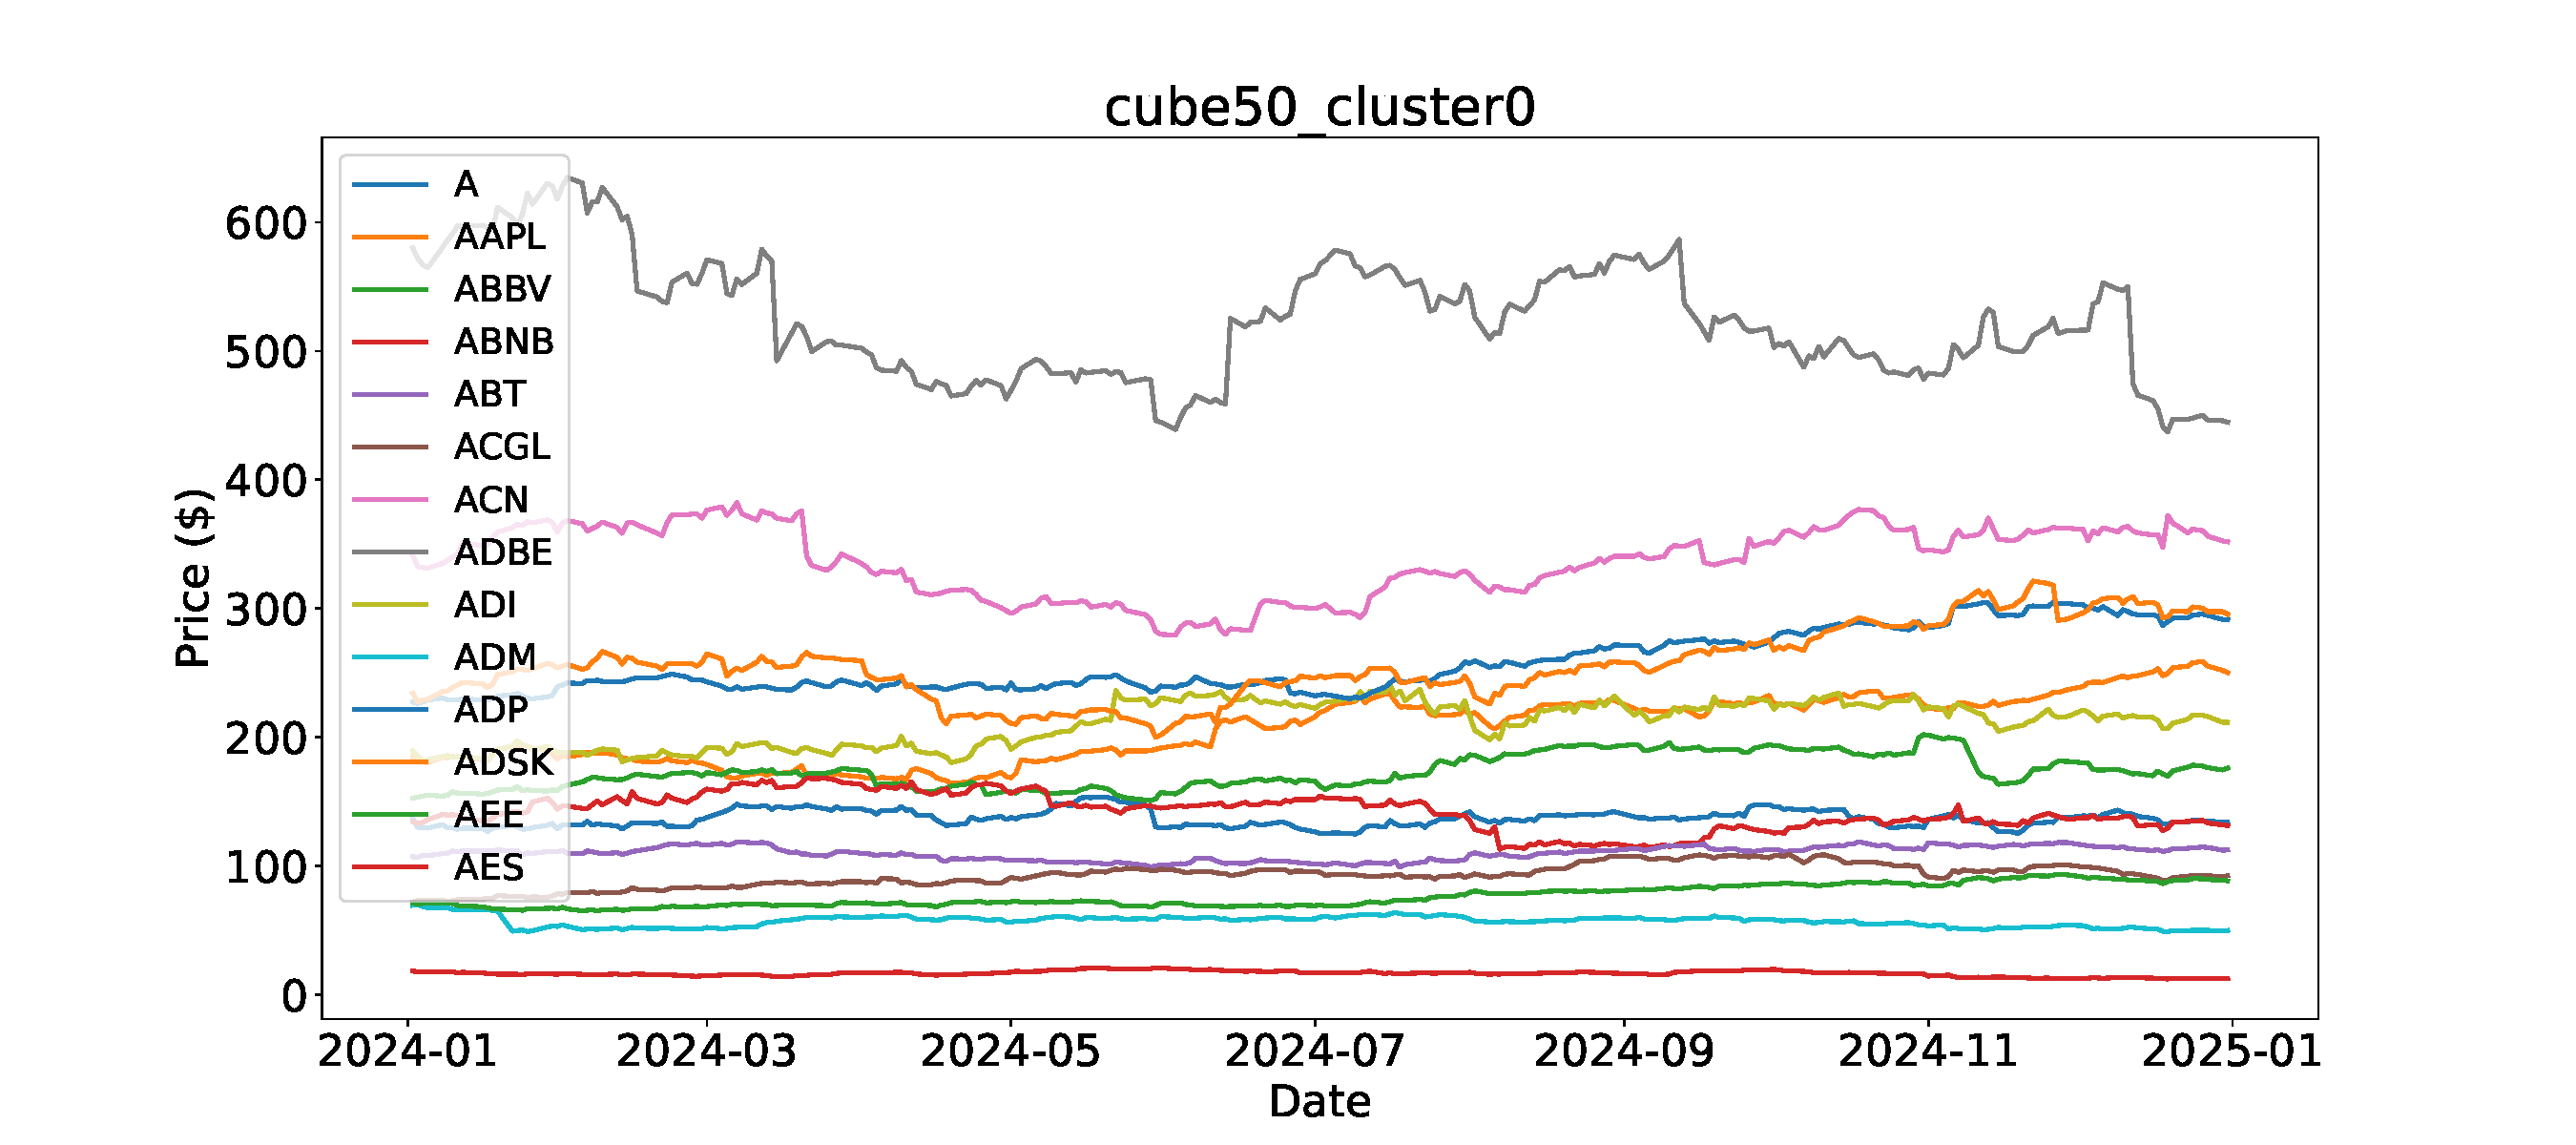
\includegraphics[width=14cm, height=10cm]{mapper_volatility_low_projection=UMAP_n_cubes=10_perc_overlap=0.1_clusterer=DBSCAN_scaler=MinMaxScaler.pdf}
  \caption{Cluster of tickers with the lowest maximal volatility.}
  \label{fig:mapper_volatility_low}
\end{figure}

We can contrast it with the bright yellow clusters, the ones with the highest maximal volatility, in \ref{fig:mapper_volatility_high}.

\begin{figure}[h!]
  \centering
  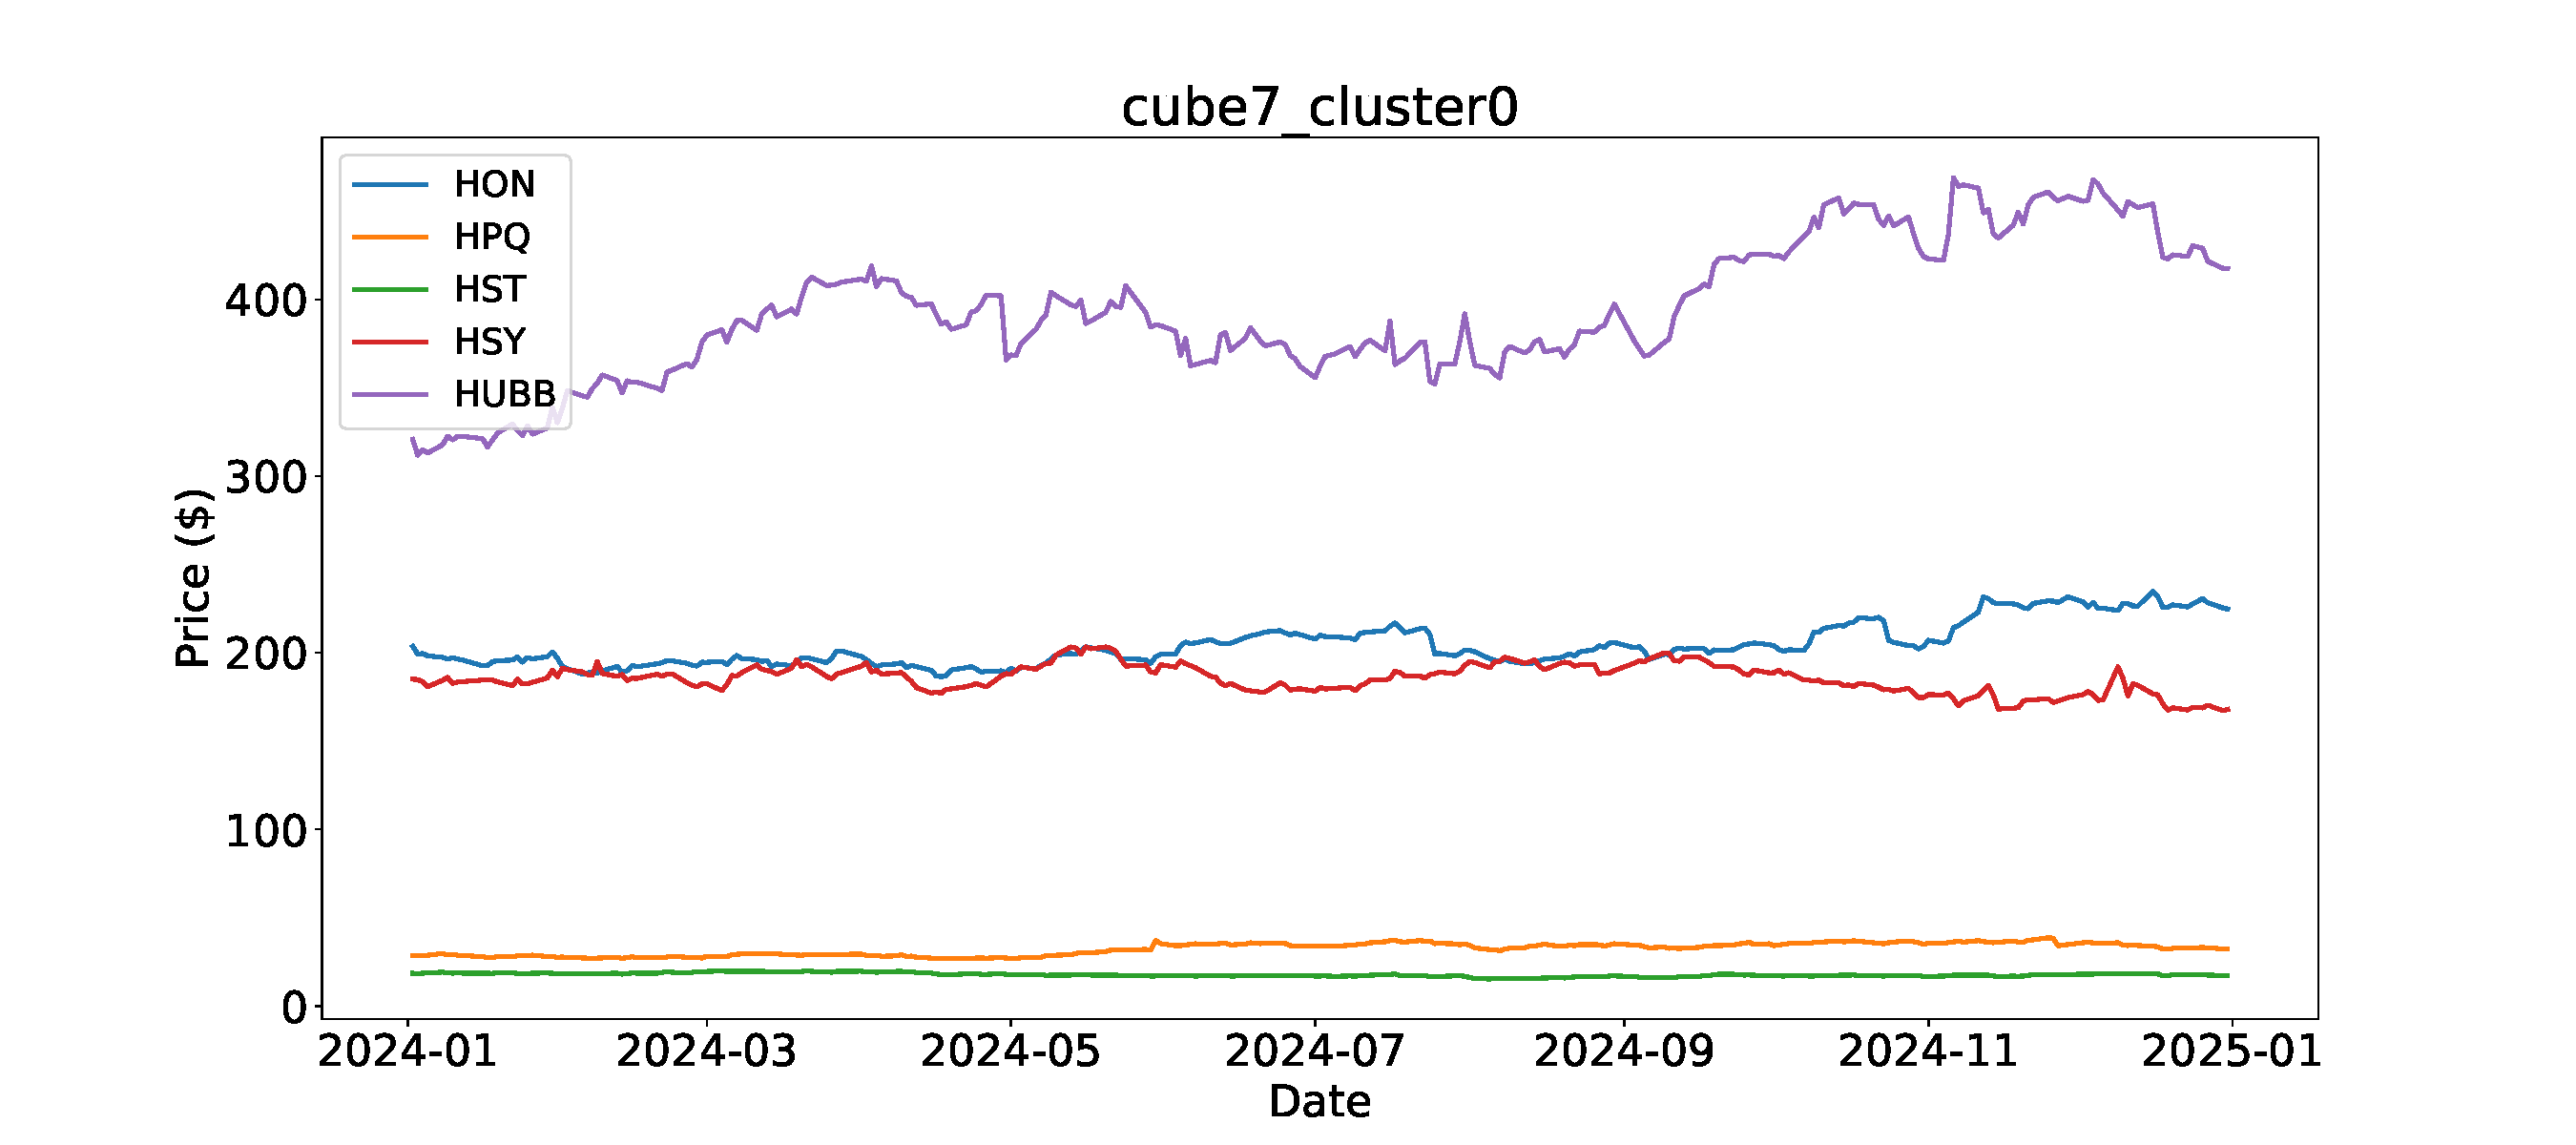
\includegraphics[width=14cm, height=10cm]{mapper_volatility_high_projection=UMAP_n_cubes=10_perc_overlap=0.1_clusterer=DBSCAN_scaler=MinMaxScaler.pdf}
  \caption{Cluster of tickers with the highest maximal volatility.}
  \label{fig:mapper_volatility_high}
\end{figure}

At first glance, the closing prices of the bottom four tickers do not seem highly volatile due to the wide price range we are plotting them against. Zooming on one of them, for example, HPQ -- the ticker of the HP company known for printers -- reveals a more interesting structure in \ref{fig:mapper_volatility_hpq}.

\begin{figure}[h!]
  \centering
  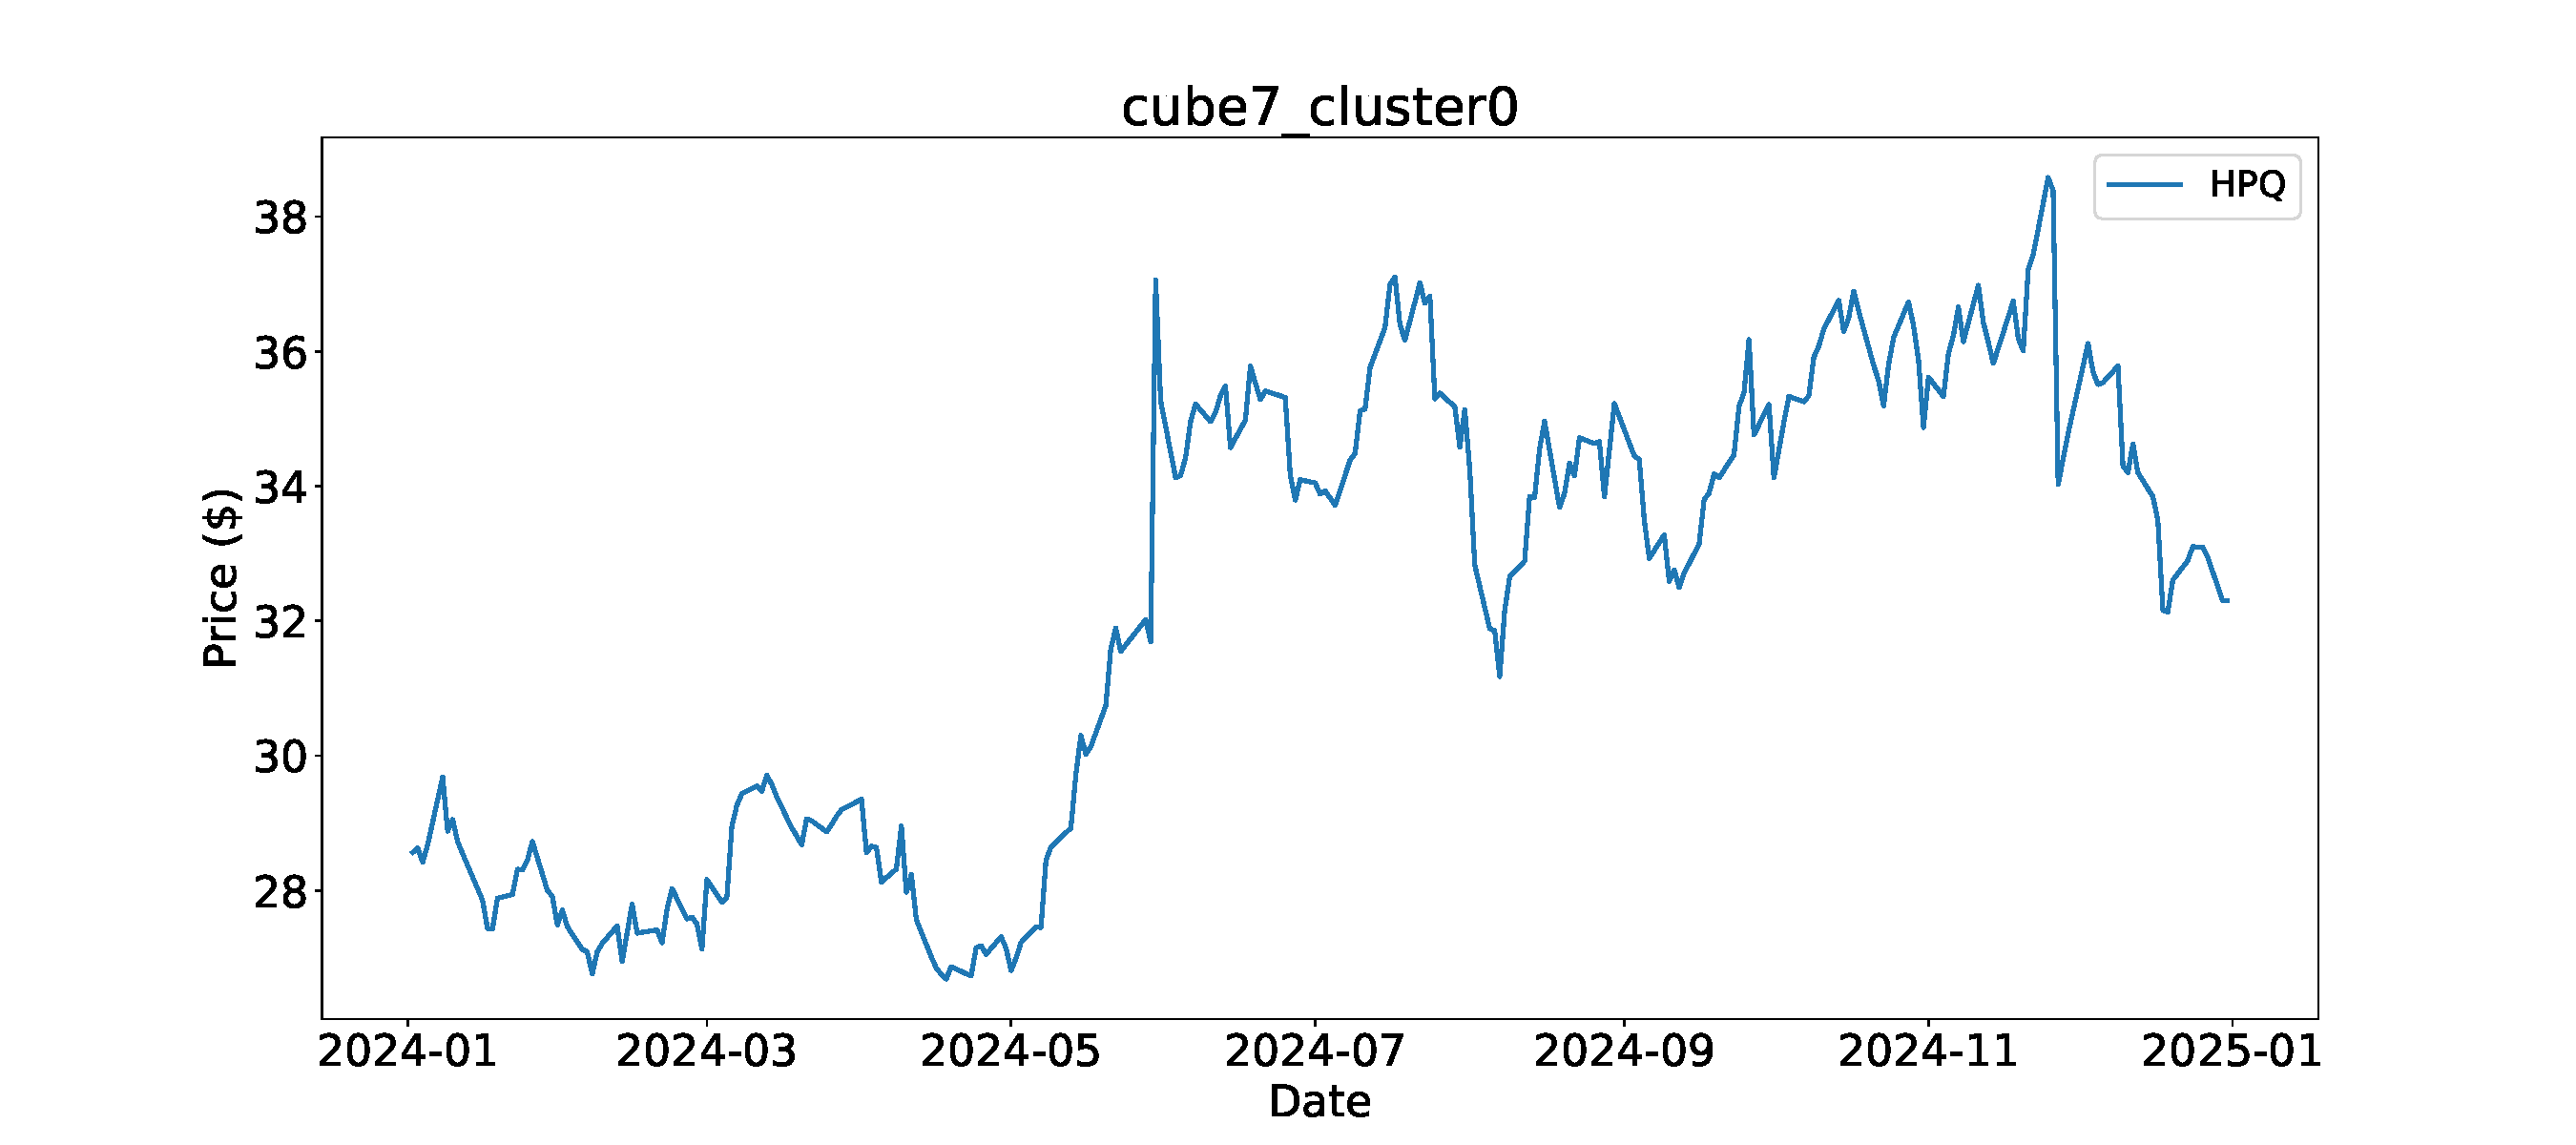
\includegraphics[width=14cm, height=10cm]{mapper_volatility_HPQ_projection=UMAP_n_cubes=10_perc_overlap=0.1_clusterer=DBSCAN_scaler=MinMaxScaler.pdf}
  \caption{Stock prices of the company HP during 2024-2025.}
  \label{fig:mapper_volatility_hpq}
\end{figure}

One could then continue with a more refined and detailed analysis of the clusters we obtained, looking into the differences and common points between them. Different coloring functions and rules could also be used, alongside other projection and clustering algorithms. All this is to show that Mapper is a powerful tool in the hands of someone with industry and theoretical knowledge of the data they have to work with, allowing them to carefully choose which algorithms, metrics and coloring functions they believe to be of importance.

\subsection{Digits dataset, revisited}

We can take a look at the digits dataset again, this time using Mapper instead of UMAP on its own. This example should highlight the fact that we can customize the resulting graph as much as we want to. In this case, we will customize the tooltips that show whenever we hover over one of the clusters. In \ref{fig:mapper_digits_custom}, we have chosen our custom tooltip function to be the images themselves, giving us the ability to directly compare the different clusters. For the projection function, we have used the t-SNE algorithm, followed by DBSCAN to do the clustering. The color function here is the label of the digit, and we kept the default rule of assigning the mean color to the cluster. This gives us a nice separation of the digits, all differentiated by a different color value. In the top right corner, we can see a cluster with multiple colors where different digits were blurred enough for DBSCAN to consider them as equal. Our custom tooltip can immediately show us which digits we are looking at.

\begin{figure}[h!]
  \centering
  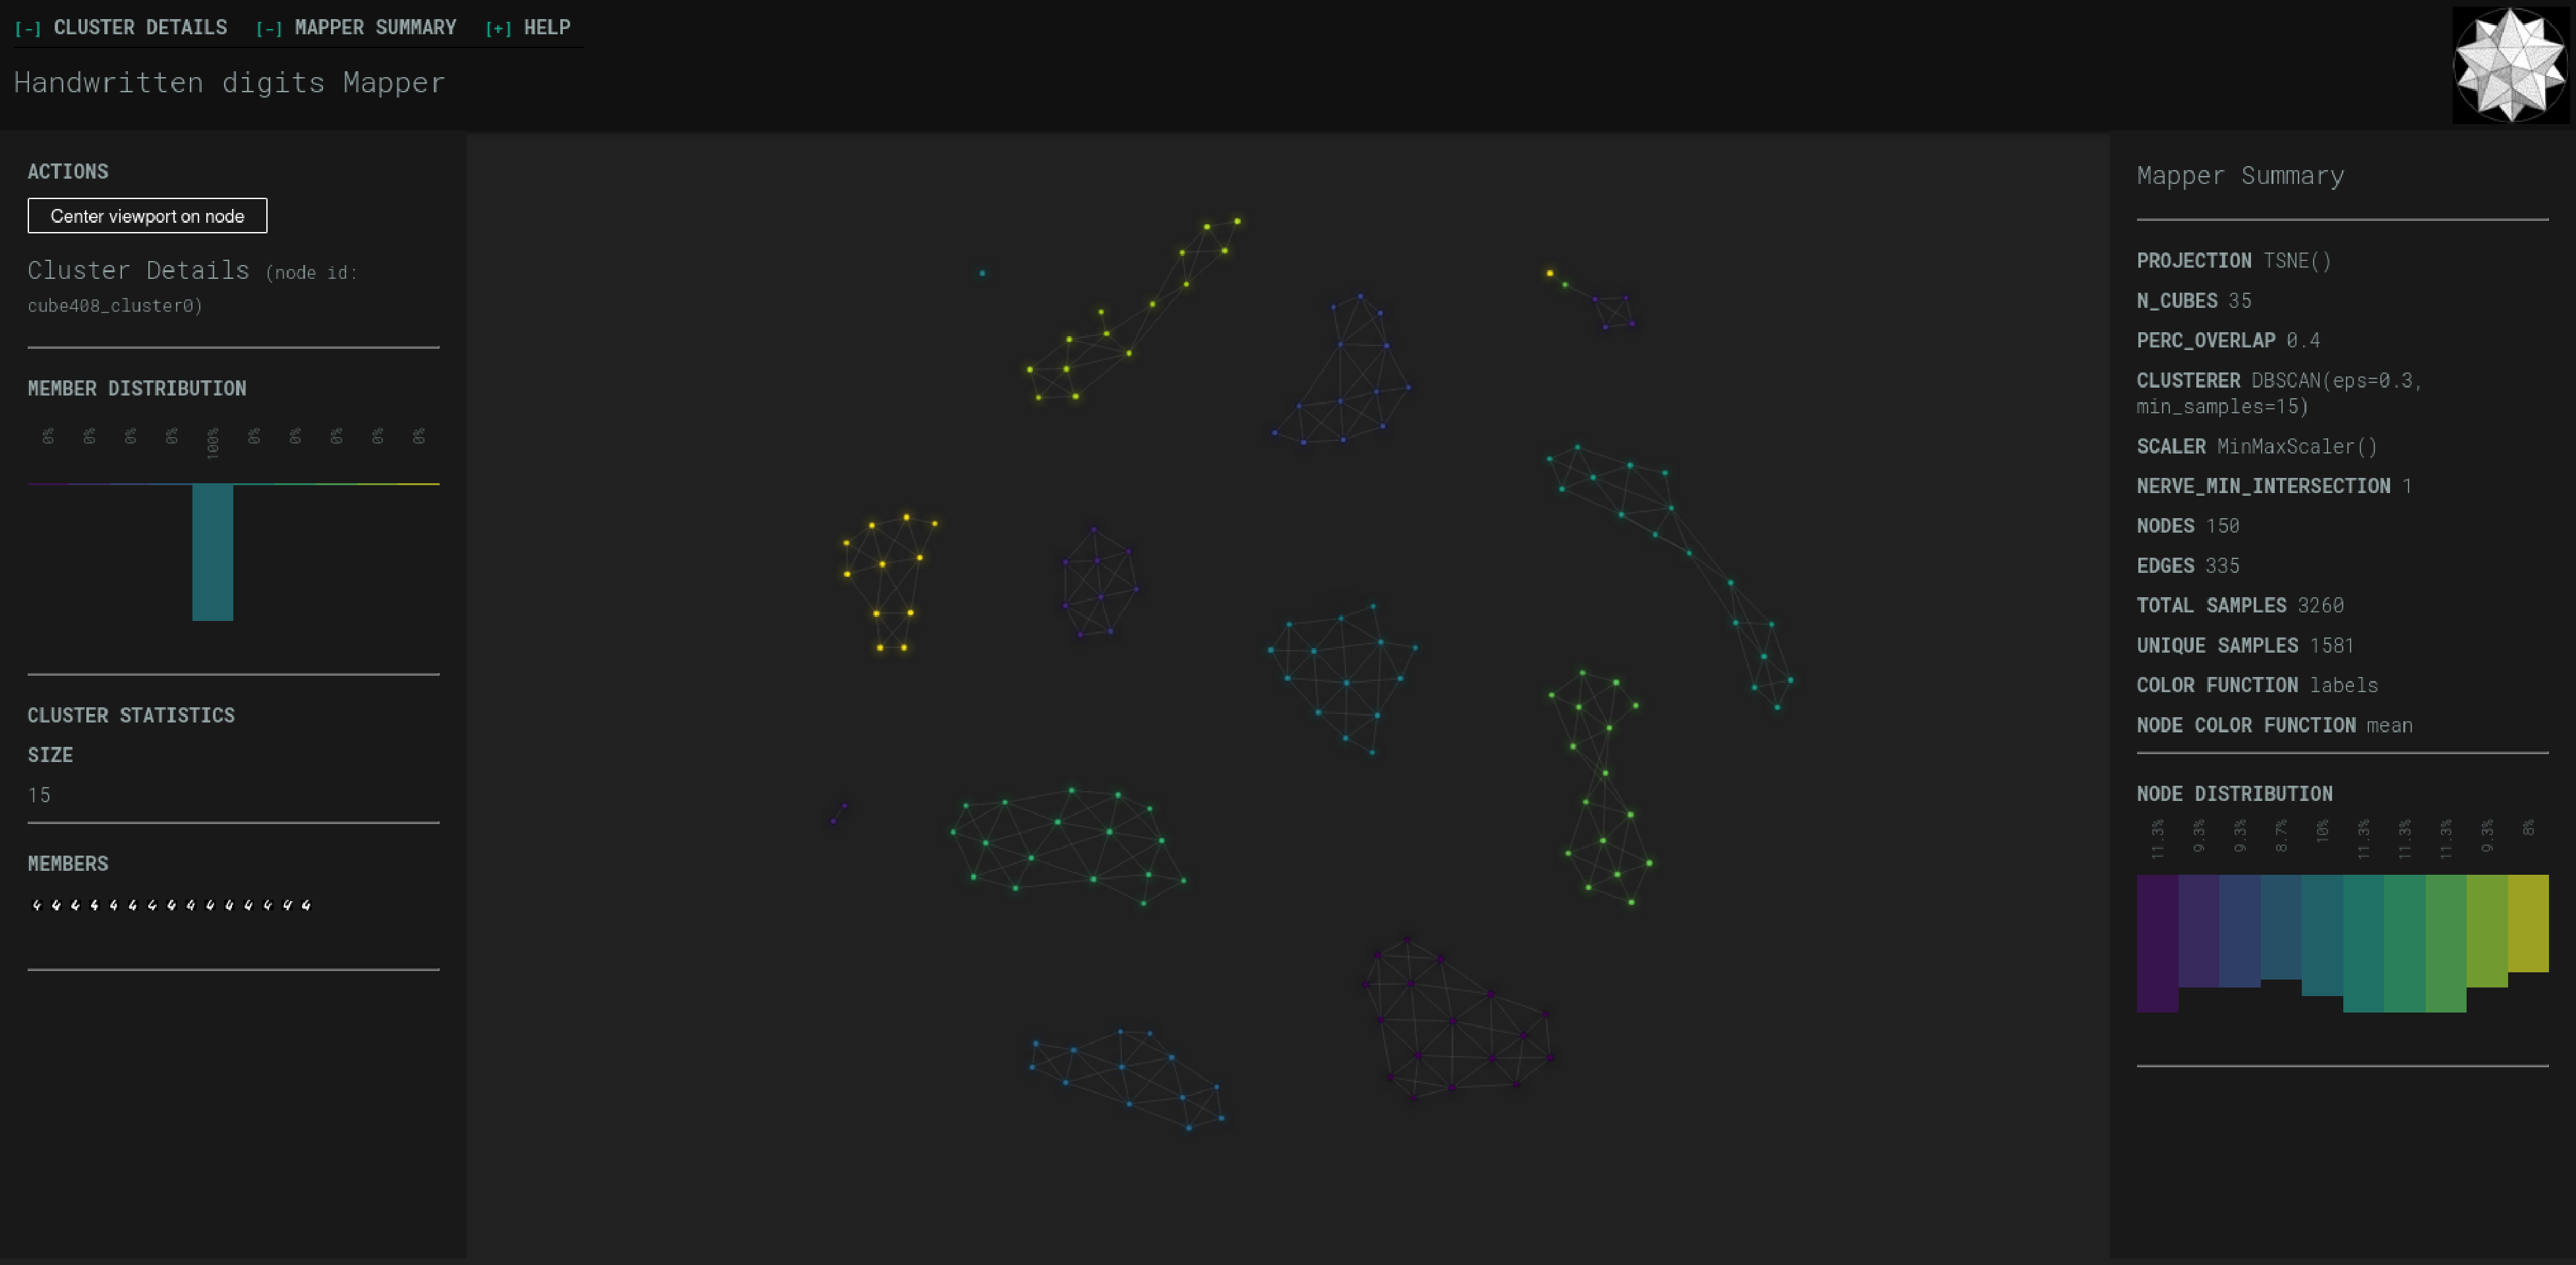
\includegraphics[width=14cm, height=10cm]{Mapper_digits_custom.pdf}
  \caption{Mapper graph of the digits dataset with a custom tooltip function.}
  \label{fig:mapper_digits_custom}
\end{figure}

We can compare this with the Mapper graph, where our tooltip function is the label of the digit, as seen in \ref{fig:mapper_digits_labels}. This won't reveal any new information, but it could be useful to compare the label of the digit with the image when the blur makes the digit illegible. The \textit{html} files for the two graphs can be located in the \textit{figures/} folder.

\begin{figure}[h!]
  \centering
  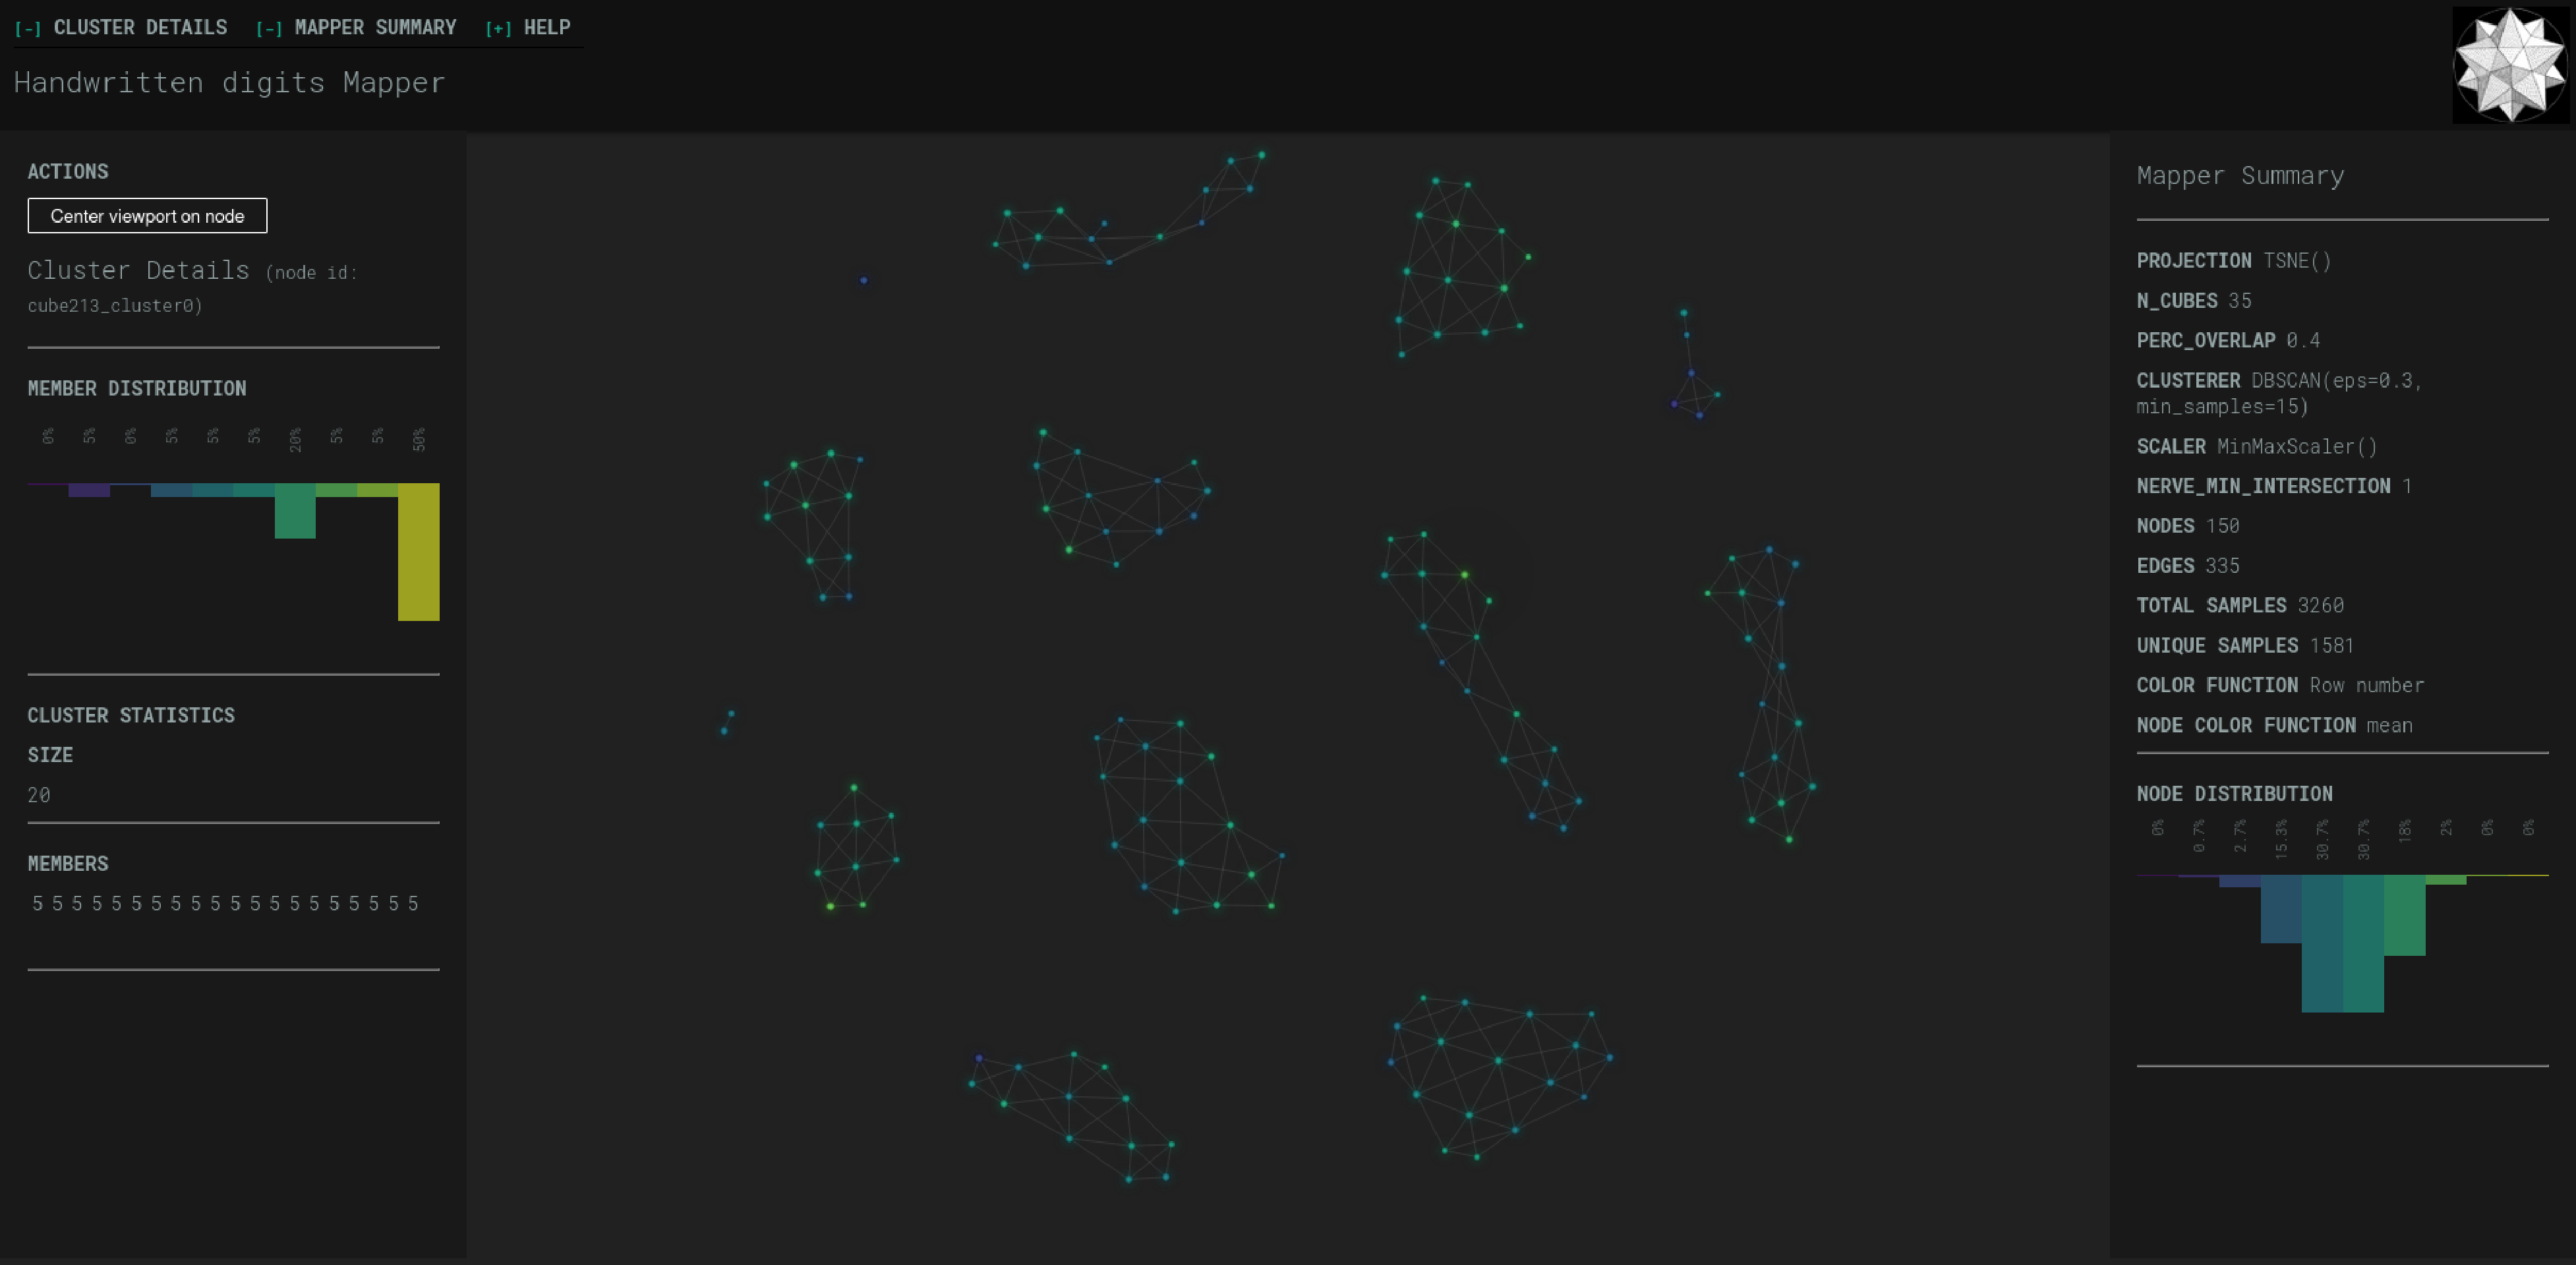
\includegraphics[width=14cm, height=10cm]{Mapper_digits_labels.pdf}
  \caption{Mapper graph of the digits dataset with labels.}
  \label{fig:mapper_digits_labels}
\end{figure}

\section{Persistent homology in practice}
At last, we can start with an example where we will compute homology groups of the datasets at hand. The key takeaway here should be that persistent homology alone usually doesn't reveal all the information that we would need. Instead, we use it to extract topological features from a dataset, vectorize them and send them into a machine learning pipeline as additional training data. If used correctly, topological features can improve the performance and precision of your model, leading to superior results. The downside is the high computational cost of the procedure, making this approach not viable for datasets in the order of millions of rows and above.

\subsection{Digits, one the last time}
We will revisit the digits dataset again, this time using persistent homology to build a \textit{scikit} classifier. As we will see in the examples to follow, persistent homology is usually used to extract topological features that can be later used in standard machine learning algorithms or statistical analysis. We have 70,000 images, each having 784 features representing a pixel intensity. The first task is to reshape the vectors into arrays of dimension 28x28. To save computational time, we will work with a smaller subset again. We split the full dataset into a training and testing dataset of sizes 60 and 10, respectively.

Because images are made of pixels and are not point clouds, we use filtrations of cubical complexes instead of simplicial ones. Ignoring technical details, all that this does is replace simplices with little cubes. The homology groups carry the same meaning as before. It simply turns out that when working with images, using cubes is more natural than using a simplicial object. To use cubical complexes, the filtrations are built from binary images, forcing us to convert the grayscale image to binary by applying a threshold to the pixel values. In this example here, we used a threshold of 0.4.

Given a binary image $\mathcal{B}$ of some digit, we will use the \textit{radial filtration} $\mathcal{R}$, which assigns to each pixel $p$ a value corresponding to the distance from some predefined center $c$ of the image

\begin{equation*}
  \mathcal{R}(p) =
  \left\{
    \begin{array}{ll}
      ||c-p||_{2} & \mbox{if } \mathcal{B}(p) = 1 \\
      \mathcal{R}_{\infty} & \mbox{if } \mathcal{B}(p) = 0
    \end{array}
  \right.
\end{equation*}
where $\mathcal{R}_{\infty}$ is the distance of the pixel that is the furthest from $c$. To reproduce the filtered images from the original article, we have chosen $c$ to be the point $c = (20, 6)$. Applying the radial filtration $\mathcal{R}$, we effectively transform the binary image into a grayscale one, with pixel values increasing as you move further away from the point $c$. These pixel values can be used to define a filtration of cubical complexes $\{K_{i}\}$, where $K_{i}$ contains all pixels with values less than the $i-$th smallest pixel value in the grayscale image. In later examples, we will see that this is what we call the sublevel set filtration of the image's cubical complex.

Once we have created our filtration, computing the persistent homology of it is straightforward. For example, if we take an image corresponding to the digit 8, its homology groups are found in \ref{fig:img8_cubical}.

\begin{figure}[h!]
  \centering
  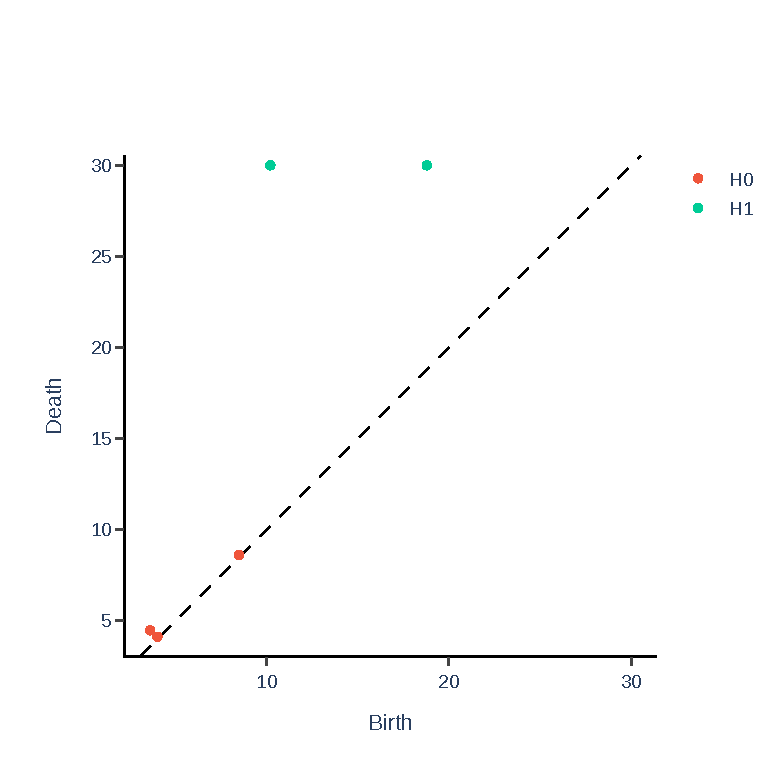
\includegraphics[width=11cm, height=10cm]{img8_cubical.pdf}
  \caption{Cubical persistence homology of the digit 8.}
  \label{fig:img8_cubical}
\end{figure}

Our sanity check works -- we see two $H_{1}$ generators corresponding to the two loops in the digit 8 and a single $H_{0}$ for the single connected component. Most methods require some sort of scaling for better results, which we can do with the persistence diagram as well, see \ref{fig:img8_cubical_scaled}.

\begin{figure}[h!]
  \centering
  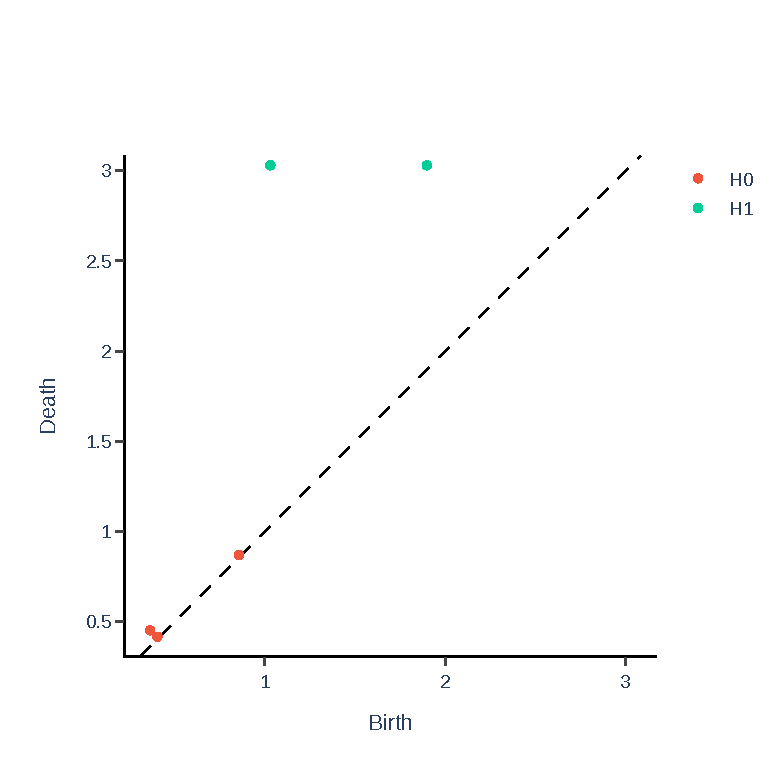
\includegraphics[width=11cm, height=10cm]{img8_cubical_scaled.pdf}
  \caption{Scaled cubical persistence homology of the digit 8.}
  \label{fig:img8_cubical_scaled}
\end{figure}

The final step is to vectorize our persistence diagrams, since most machine learning pipelines only accept an array of vectors. This can be achieved in multiple ways. For our single image of the digit 8, we used a Gaussian kernel and convolved the diagram with it. From this, we managed to extract a vector of amplitudes. While this was done for a single image, we may want to extract a variety of features over the whole training dataset.

To do this, we can augment our radial filtration with a \textit{height filtration} $\mathcal{H}$, which is defined by choosing a vector $v \in \mathbb{R}^{2}$ representing a direction and by assigning values $\mathcal{H}(p) = \langle p, v \rangle$ based on the distance of $p$ to the hyperplane defined by $v$. We will pick a uniform set of directions and centers for our filtrations, as we lack any prior information that could guide our investigation. Our method of generating features from the persistence diagrams will be what we call \textit{persistence entropy}. This is simply the entropy of the points of the diagram. More specifically, the persistence entropy of a diagram $D$ is defined by
\begin{equation*}
  E(D) = -\sum_{i \in I}p_{i}\:\log(p_{i}),
\end{equation*}
where
\begin{equation*}
  p_{i} = \frac{d_{i}-b_{i}}{L_{D}} \quad \text{and} \quad L_{D} = \sum_{i \in I}(d_{i}-b_{i}),
\end{equation*}
where $d_{i}$ and $b_{i}$ are the death and birth times of the equivalence classes.

Doing all of this, we managed to extract 476 topological features per image. Some of the features will be highly correlated, and normally you would want to filter those out. Despite all of that, we can now happily send them into a Random Forest classifier and test our accuracy. In this example, we managed to achieve an accuracy of 80\% on our small dataset, using nothing but topological features. A better result would be achieved by applying a feature selection strategy and using the original data in the classifier as well.

As a little sidenote, we may think of the choice of direction and center as hyperparameters. We can then proceed with a greedy hyperparameter search over a grid to see what the direction, homology direction and number of trees give us the best accuracy. Running the search, we found that the optimal number of trees is 500, the optimal homology dimension is $H_{0}$ and the optimal filtration direction is the vector $[1, 0]$. This intuitively makes sense when we compare the digits 6 and 9 with each other.

The notebook with the entire pipeline can be found in the \textit{scripts/} directory under the name \textit{Digits\_classification.ipynb}.

\subsection{Sublevelset filtration in general}
In this section, we will construct our filtrations ourselves, specifically the sublevelset filtration (sometimes also called the lower star filtration) of some topological space. It is a stable way of describing and looking for critical points -- local minima and maxima. This will be immediately clear when we start working with time series or signals but the approach will be demonstrated on data like images as well.

Intuitively, we compute the null homological group $H_{0}$ of the connected components that are constructed when a ``rising pools of water'' slowly fill out the space. When a new pool is formed at a local minimum, a class is born; when two pools merge together at a local maximum, the class dies.

\subsubsection{Time Series}
We will start with a simple example of a periodic time series where the local minima and maxima are visible. The function we will work with can be seen on \ref{fig:cosine_period}.

\begin{figure}[h!]
  \centering
  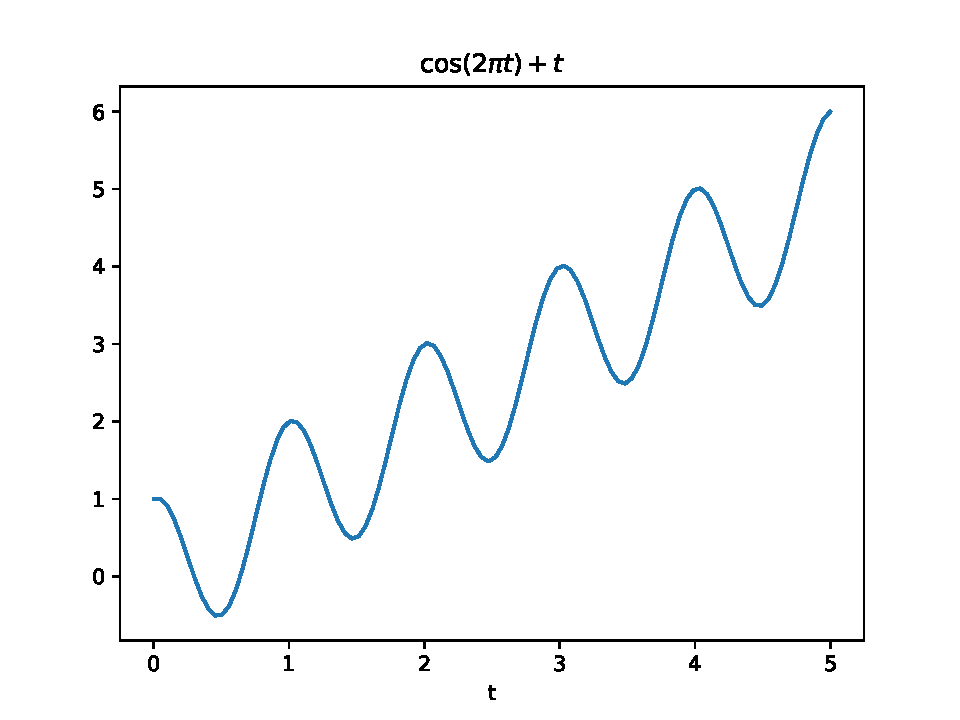
\includegraphics[width=12cm, height=10cm]{Cosine_period.pdf}
  \caption{The periodic signal $\cos(2\pi t) + t$.}
  \label{fig:cosine_period}
\end{figure}

The next step is to construct a sparse distance matrix to perform the sublevelset filtration. This has the added benefit of decreased computational cost due to the sparsity and a more fine-grained control of how we build the complex. For each point of the time series there is a vertex, which is born at the height of the point in the time series. This represents the initial state of the filtration. Since we are interested in the sublevelset filtration, we will add edges at a height equal to the larger of the two heights of the vertices they connect. The edges naturally connect adjacent points in the time series since, usually, we measure the signal in time and time only goes from left to right.

In more practical terms, we add the vertex birth times along the diagonal of the distance matrix. Once we have our distance matrix, we can directly pass it as input for the computation of the persistence diagram. With some minor graphical touches, we can plot the results side-by-side in \ref{fig:cosine_filtration}.

\begin{figure}[h!]
  \centering
  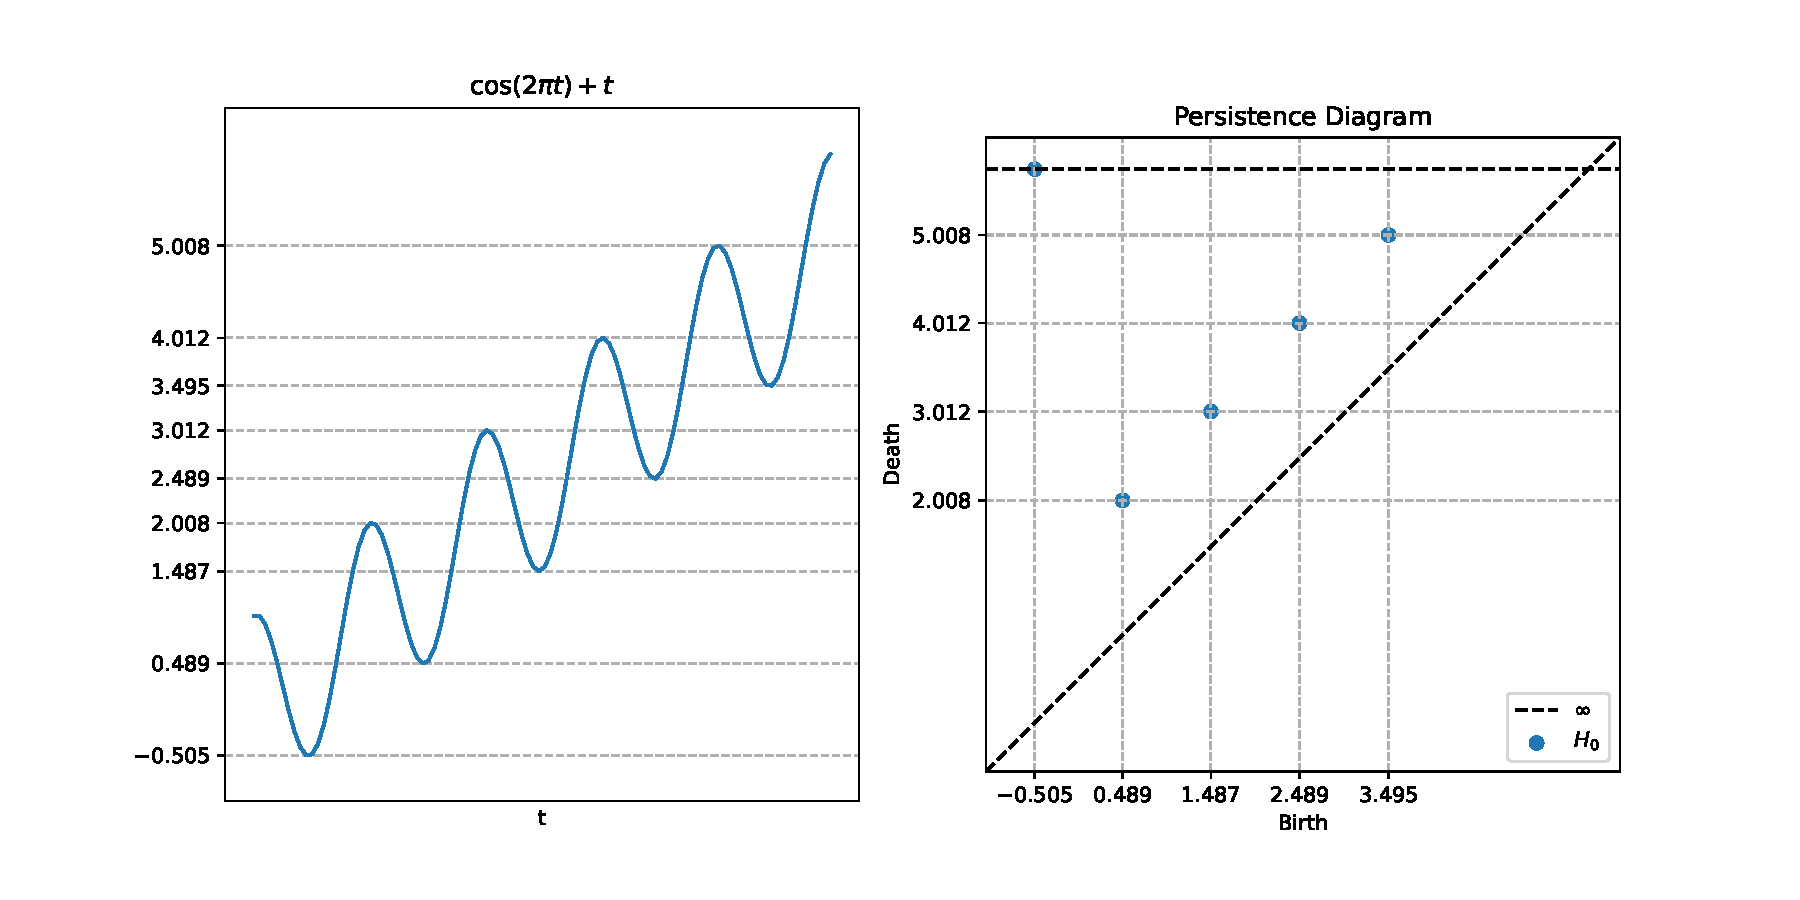
\includegraphics[width=15cm, height=10cm]{sublevelset_cosine.pdf}
  \caption{The sublevelset filtration of the signal.}
  \label{fig:cosine_filtration}
\end{figure}

We see that the birth times of the individual homology classes here nicely map to the local minima of the signal, while the death times map to the local maxima in a 1-to-1 correspondence. We could do the opposite, filling the ``pools of water'' from the top instead and this would give us the superlevelset filtration of the time series. Of course, this amounts to calculating the sublevelset filtration of the same function but with a flipped sign in front.

\subsubsection{Image Filtrations}

Sublevelset filtration of images works in the exact same manner, allowing us to explore local minima as birth times and saddle points as death times while looking at the zero-dimensional homology groups. The definition of the function that provides the filtration is in the same spirit as with the time series -- we construct a sparse distance matrix in which every pixel in the image is a vertex. Every vertex is connected to its 8 neighbors (or fewer, if it is a boundary pixel). The function value on the edge is taken to be the maximum of the two pixel values it connects. We can start with a simple image containing some Gaussian blobs, see \ref{fig:blobs_example}. There are three negative Gaussians present; one reaching its minimum at -3, the other at -2 and the last at -1.

\begin{figure}[h!]
  \centering
  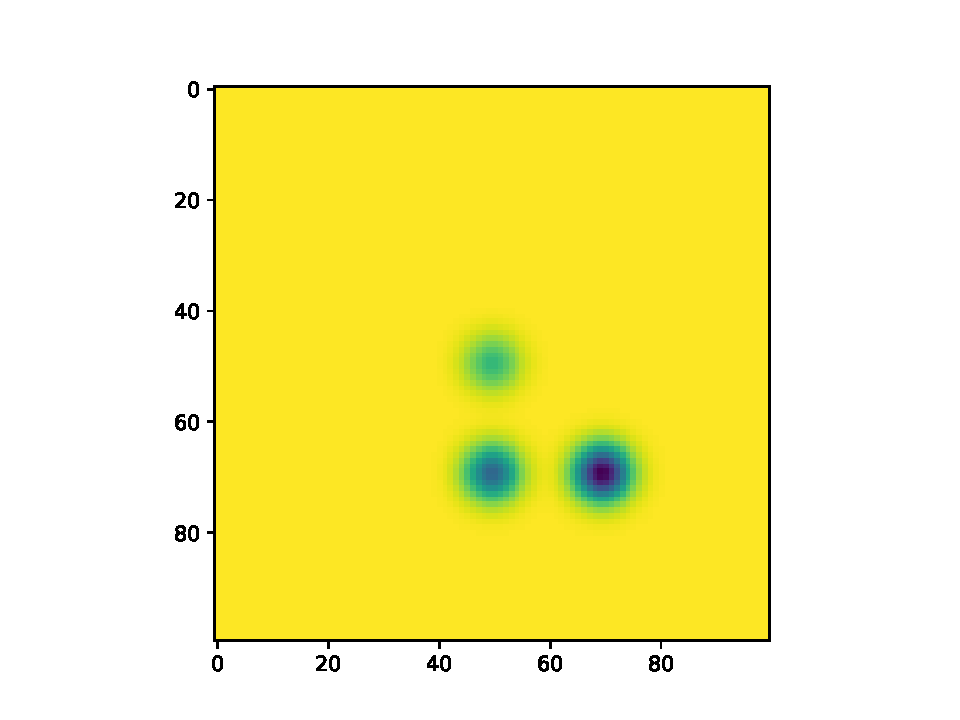
\includegraphics[width=13cm, height=10cm]{sublevelset_img.pdf}
  \caption{Image containing some Guassian blobs.}
  \label{fig:blobs_example}
\end{figure}

For images, there already exists a pre-built function that we can use instead of writing it ourselves. Computing the persistence diagram of this image gives us \ref{fig:blobs_diagram}. Just like with the time series example, the three dots correspond to each of the 3 Gaussians, each of which is born at the respective local minimum. Two of them die around 0 and the third is born at -3, absorbing all classes into itself and never dying.

\begin{figure}[h!]
  \centering
  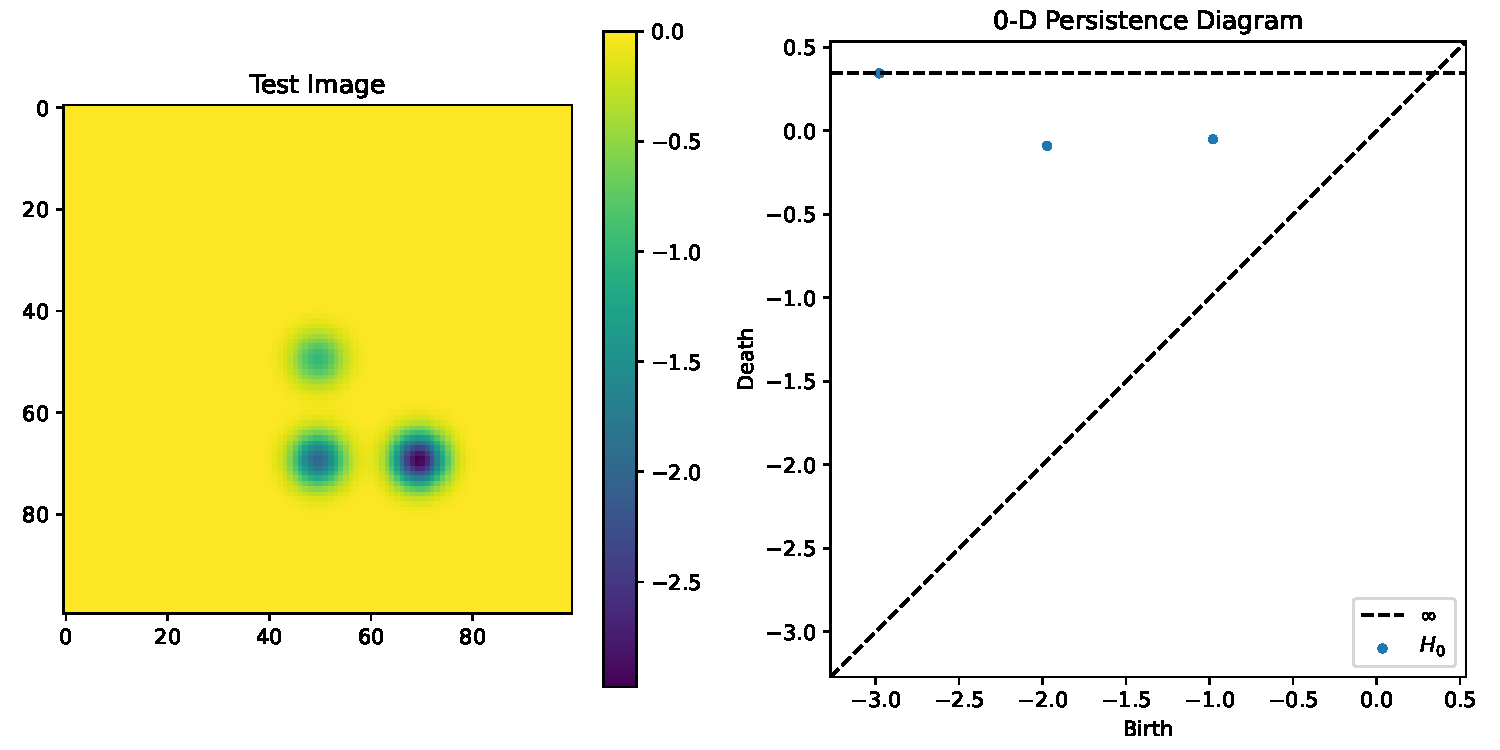
\includegraphics[width=15cm, height=10cm]{sublevelset_img_diagram.pdf}
  \caption{The result of taking the sublevelset filtration of the Gaussian blobs.}
  \label{fig:blobs_diagram}
\end{figure}

Let us look at a slightly more exciting example in \ref{fig:cells}. Here we have a zoomed up image of some wood cells. The first step is to convert this image to a grayscale one. Doing so, we see that the interiors of the cells have high values. They also meet a saddle point somewhere on their boundary with a value close to 0. We want to ideally identify the interiors of the cells in an automated fashion. Since this is our goal, we are interested in a local maximum of large persistence within each cell; that is, we want to perform superlevelset filtration of the image.

\begin{figure}[h!]
  \centering
  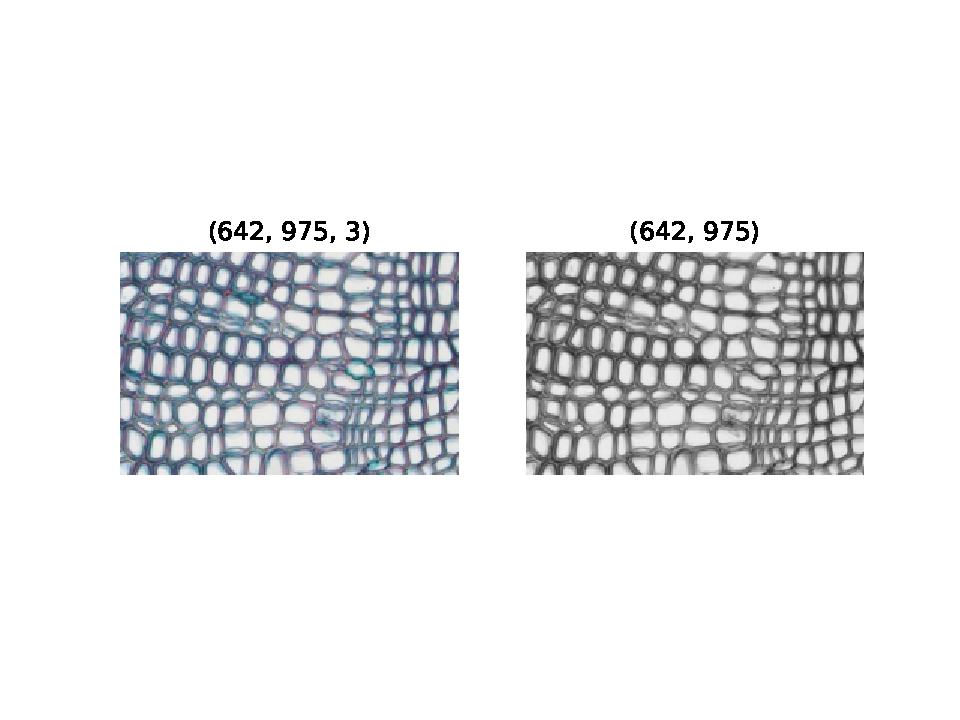
\includegraphics[width=10cm, height=10cm]{sublevelset_cells.pdf}
  \caption{Example image of wood cells.}
  \label{fig:cells}
\end{figure}

But as mentioned above, we don't need to hack a suboptimal solution; we can simply pass the negative of the image and compute its sublevelset filtration instead. The result of this we can see in \ref{fig:cells_diagram1}. While the diagram is a useful first step, we need to extract the cell interior in some way out of this. We can do this by selecting a persistence treshold, above which we will consider a dot to be associated to a cell.

\begin{figure}[h!]
  \centering
  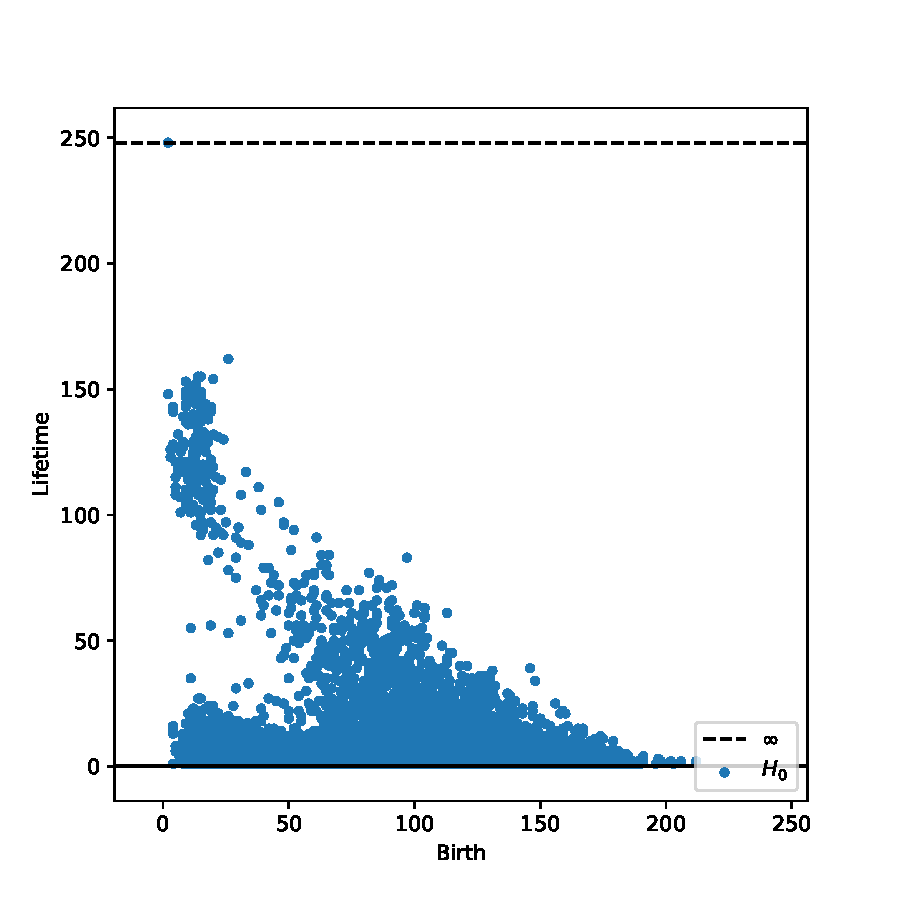
\includegraphics[width=10cm, height=10cm]{sublevelset_cells_diagram1.pdf}
  \caption{Persistence diagram of the grayscale image of the cells.}
  \label{fig:cells_diagram1}
\end{figure}

We can add some white noise to the pixels and apply a uniform filter to add a small amount of blur to the image. This would ideally increase the chance of the maximum to be closer to the center of the cell; the result of which is seen in \ref{fig:cells_smoothed}. If we compute the persistence diagram of the smoothed image, the difference is visible in \ref{fig:cells_diagram2}.

\begin{figure}[h!]
  \centering
  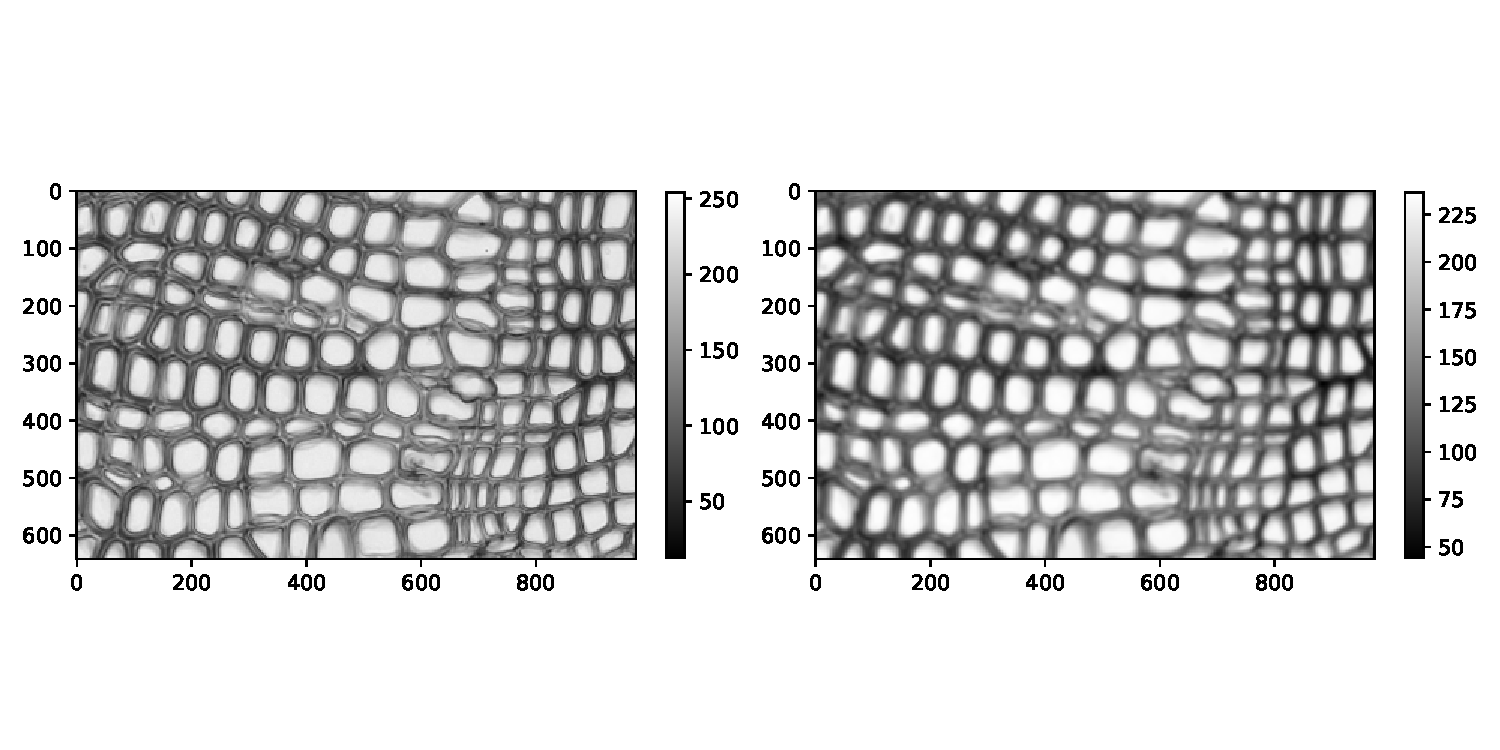
\includegraphics[width=10cm, height=10cm]{sublevelset_cells_smoothed.pdf}
  \caption{Smoothed out version of the grayscale image of the cells.}
  \label{fig:cells_smoothed}
\end{figure}

\begin{figure}[h!]
  \centering
  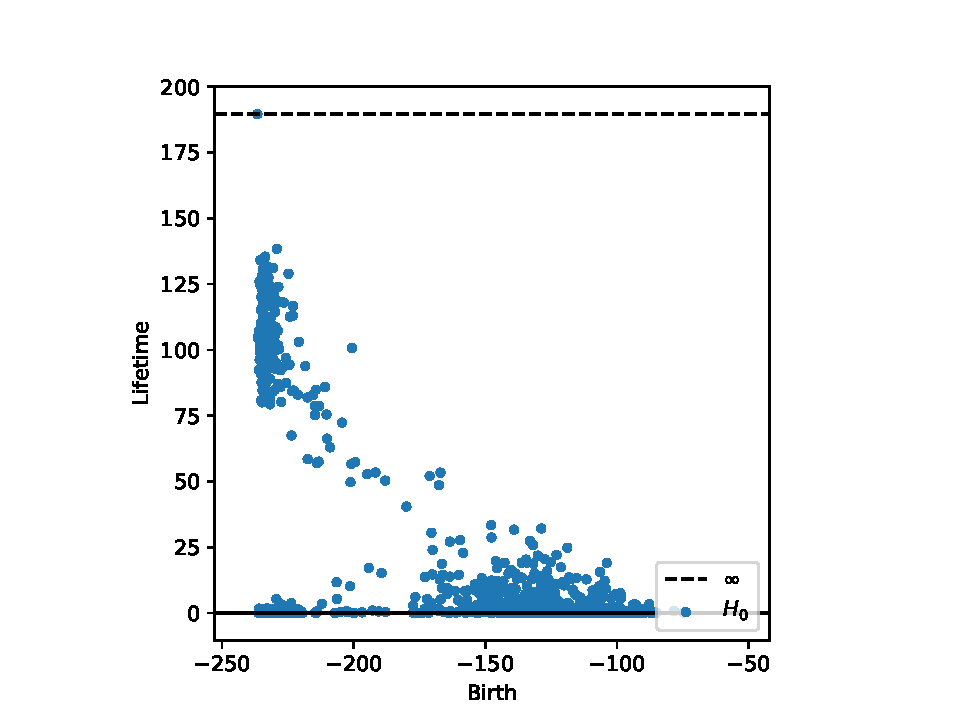
\includegraphics[width=10cm, height=10cm]{sublevelset_cells_diagram2.pdf}
  \caption{Persistence diagram of the smoothed out image.}
  \label{fig:cells_diagram2}
\end{figure}

We choose a cutoff of all points with a lifetime greater than 70 in this example. Extracting the pixel representatives satisfying this condition and plotting them in the original image results in \ref{fig:cells_filled}. Using a naive approach to the problem, we obtained reasonable results. There are cells with duplicates and some have no points at all, but most have only one. Tuning the threshold and the amount of noise added could further improve this procedure without relying on advanced algorithms from image processing.

\begin{figure}[h!]
  \centering
  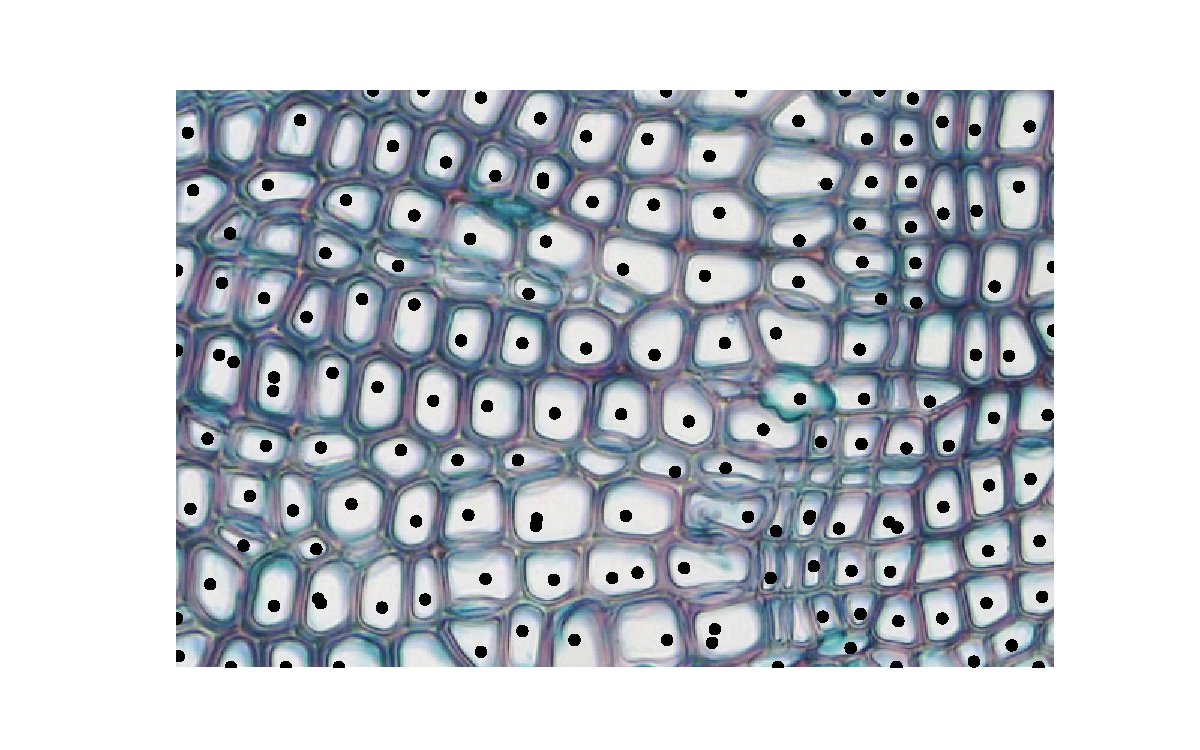
\includegraphics[width=10cm, height=10cm]{cells_filled.pdf}
  \caption{Filled out image of cells.}
  \label{fig:cells_filled}
\end{figure}

On an ending note, we can give a formal proof of the fact that a black hole really has a hole inside, using the famous image and computing its sublevelset filtration as we did above.

\begin{figure}[h!]
  \centering
  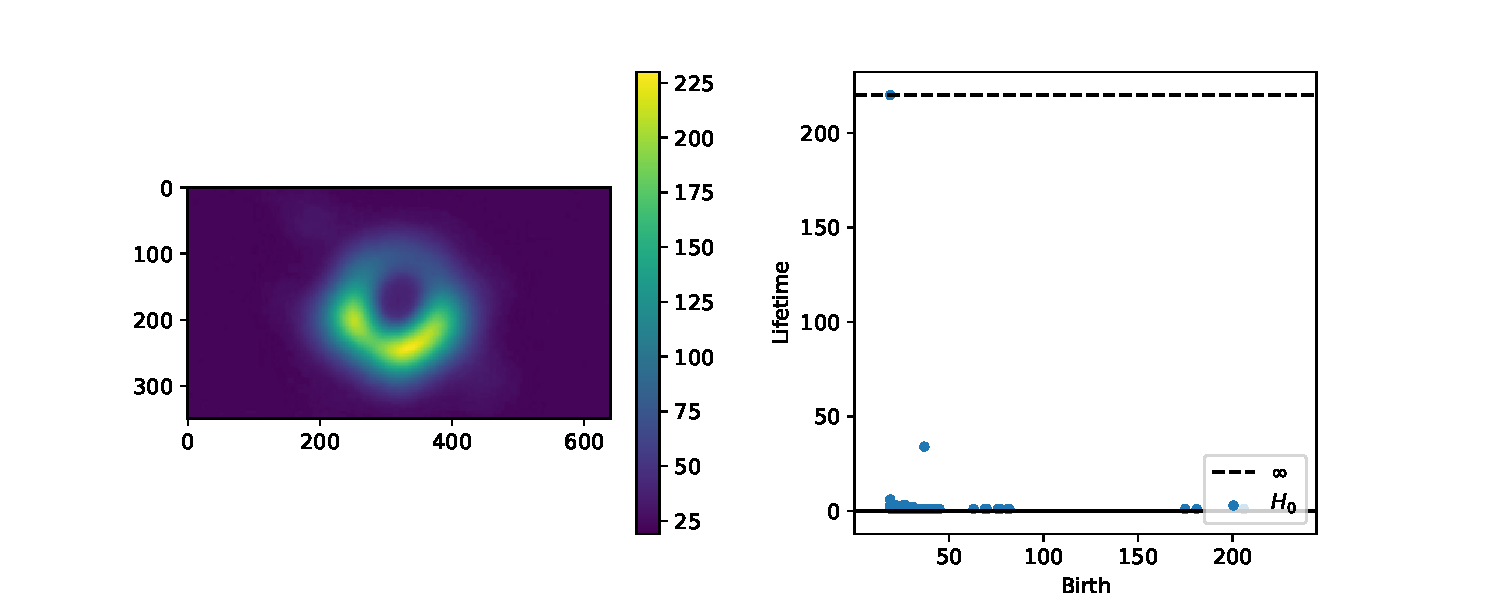
\includegraphics[width=14cm, height=7cm]{blackhole_diagram.pdf}
  \caption{Persistence diagram of a black hole.}
  \label{fig:black_hole}
\end{figure}

\subsection{Sliding Windows}

The second approach when working with time series or signals is to make use of Taken's embedding theorem and sliding windows. \cite{takens2006detecting}. A delay embedding theorem gives us condition under which we can reconstruct a chaotic dynamical system from a sequence of observations. Taken's theorem specifically gives us condition under which we can reconstruct the attractors of the dynamical system.

Using Taken's theorem, we can transform the signal into a point cloud, allowing us to directly compute its persistent homology groups without further transformations. Formally, given a time series $f(t)$, we extract vectors of the form
\begin{equation*}
f_{i} = [f(t_{i}), f(t_{i} + \tau), f(t_{i} + 2\tau), \ldots, f(t_{i} + (d-1)\tau)] \in \mathbb{R}^{d},
\end{equation*}
where $d$ is the dimension of the embedding and $\tau$ is the time delay parameter. Typically, we call the quantity $(d-1)\tau$ the \textit{window size} and the difference $t_{i+1} - t_{i}$ the \textit{stride}. The underlying idea here is, as long as $f$ has a non-trivial recurrent structure, to use Taken's theorem to construct an embedding of the signal that preserves the topological qualities and then compute its persistent homology.

We may start with a simple cosine wave. The choice of stride and window size is the hardest problem when using a sliding window technique, as it is not exactly obvious which values will give us an ``optimal'' embedding. Later we'll see that we can search for them in a automatic fashion but for now, let us choose $d=3$, $\tau=8$ and a stride of 10. With this choice of parameters, the resulting embedding in $\mathbb{R}^{3}$ is shown in \ref{fig:cosine_embedding}.

\begin{figure}[h!]
    \centering
    \subfloat[\centering The signal]{{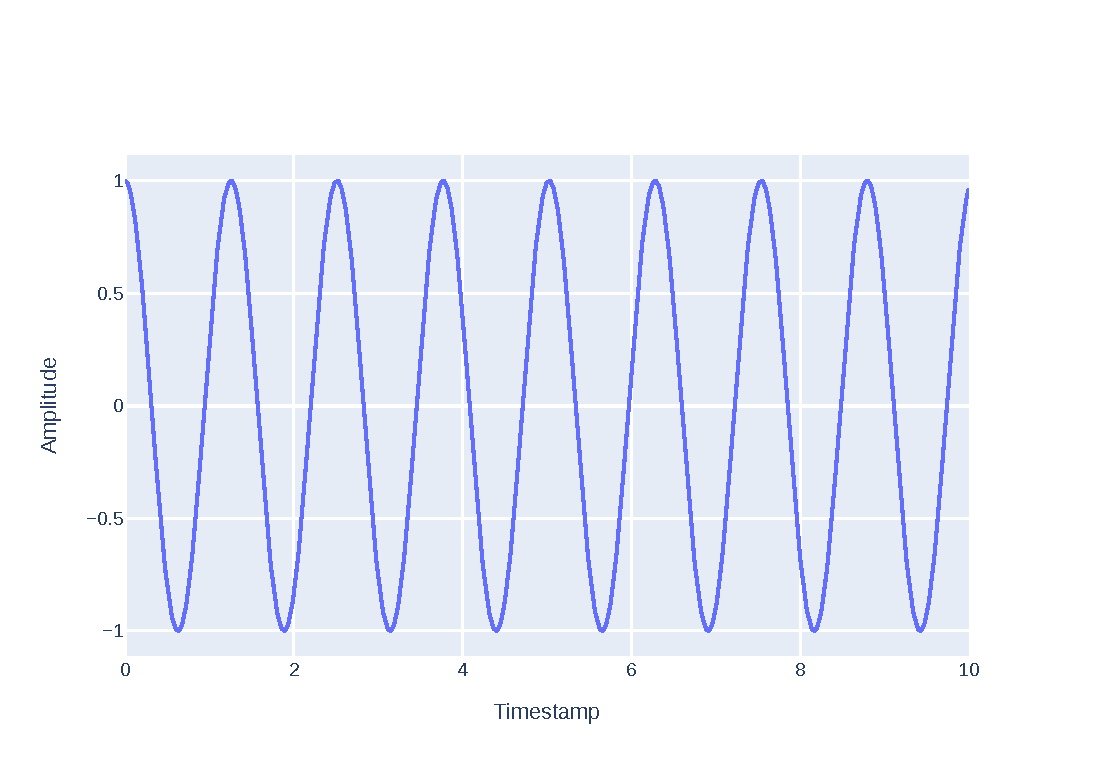
\includegraphics[width=7cm]{cosine.pdf} }}%
    \qquad
    \subfloat[\centering Its embedding in $\mathbb{R}^{3}$]{{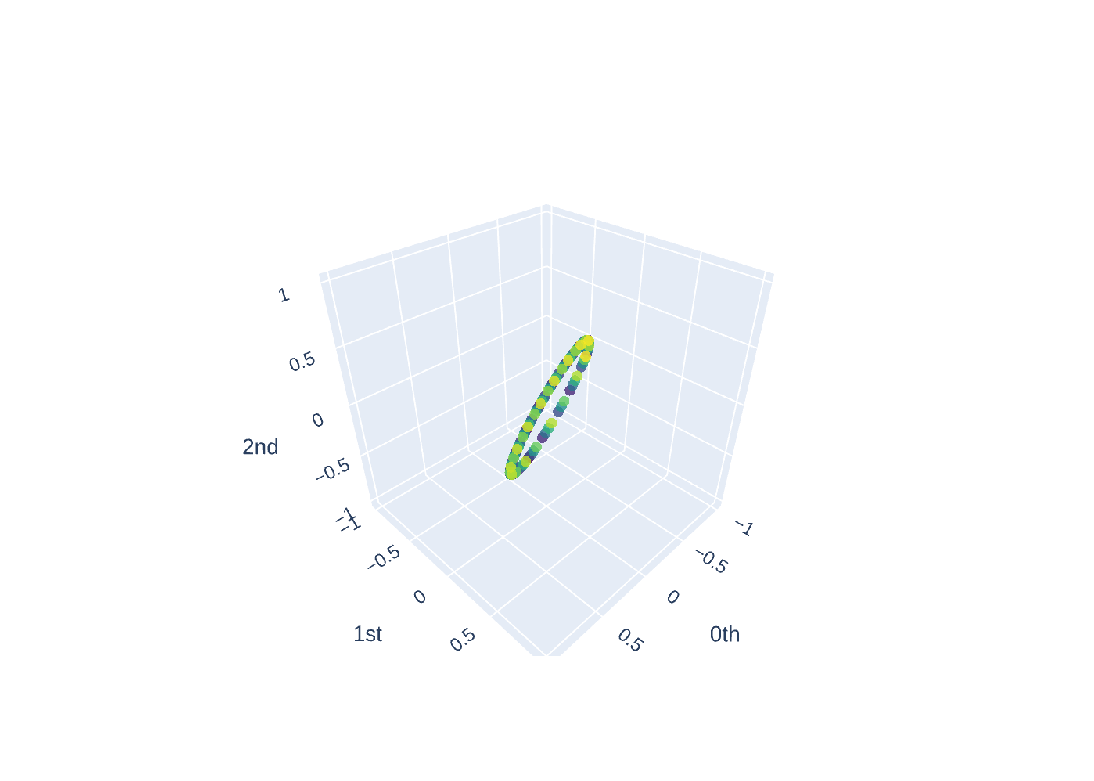
\includegraphics[width=7cm]{point_cloud1.pdf} }}%
    \caption{Ordinary cosine wave}%
    \label{fig:cosine_embedding}%
\end{figure}

We can compare this with a quasi-periodic signal of the form
\begin{equation*}
  f(t) = cos(t) + cos(\pi t),
\end{equation*}
as seen in \ref{fig:nonperiodic_embedding}, where we used $d=3$, $\tau=16$ and a stride of 3. The difference in the geometry of the embedding should be immediately clear, as in the case of the cosine wave, we have recovered a perfect elipse capturing the clean, periodic behaviour of the signal.

\begin{figure}[h!]
    \centering
    \subfloat[\centering The signal]{{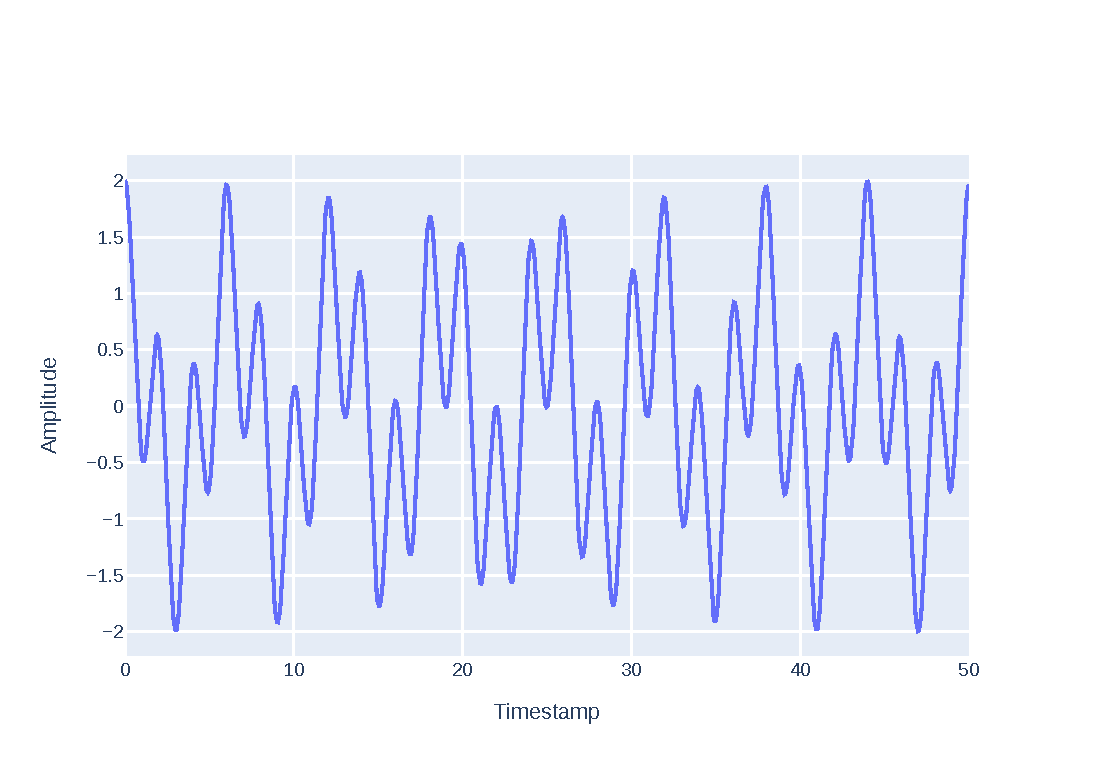
\includegraphics[width=7cm]{nonperiodic_signal.pdf} }}%
    \qquad
    \subfloat[\centering Its embedding in $\mathbb{R}^{3}$]{{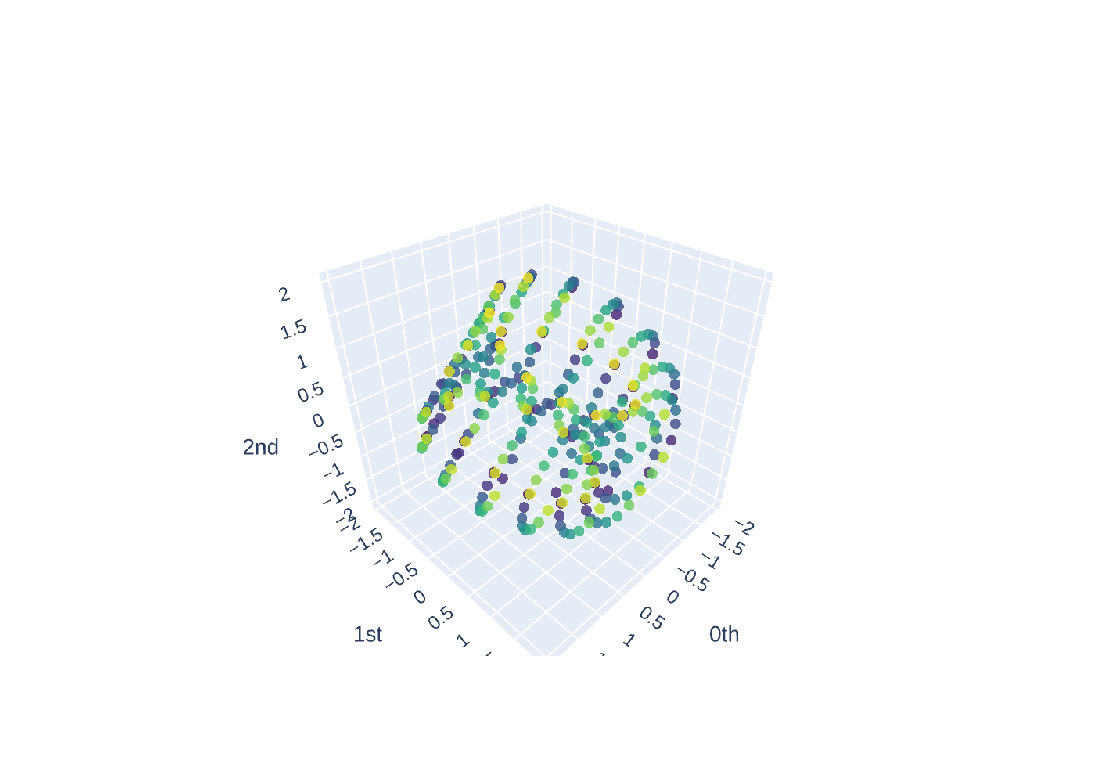
\includegraphics[width=7cm]{point_cloud2.pdf} }}%
    \caption{Quasi-periodic wave}%
    \label{fig:nonperiodic_embedding}%
\end{figure}

We can confirm this by looking at the persistence diagrams that we compute from the embeddings in \ref{fig:embedding_diagrams}. In the first diagram, we see a single point associated with the $1-$dimensional persistent homology. This represents the single loop found in the embedding and is a direct consequence of the periodic nature of the signal.

\begin{figure}[h!]
    \centering
    \subfloat[\centering Diagram for the periodic wave]{{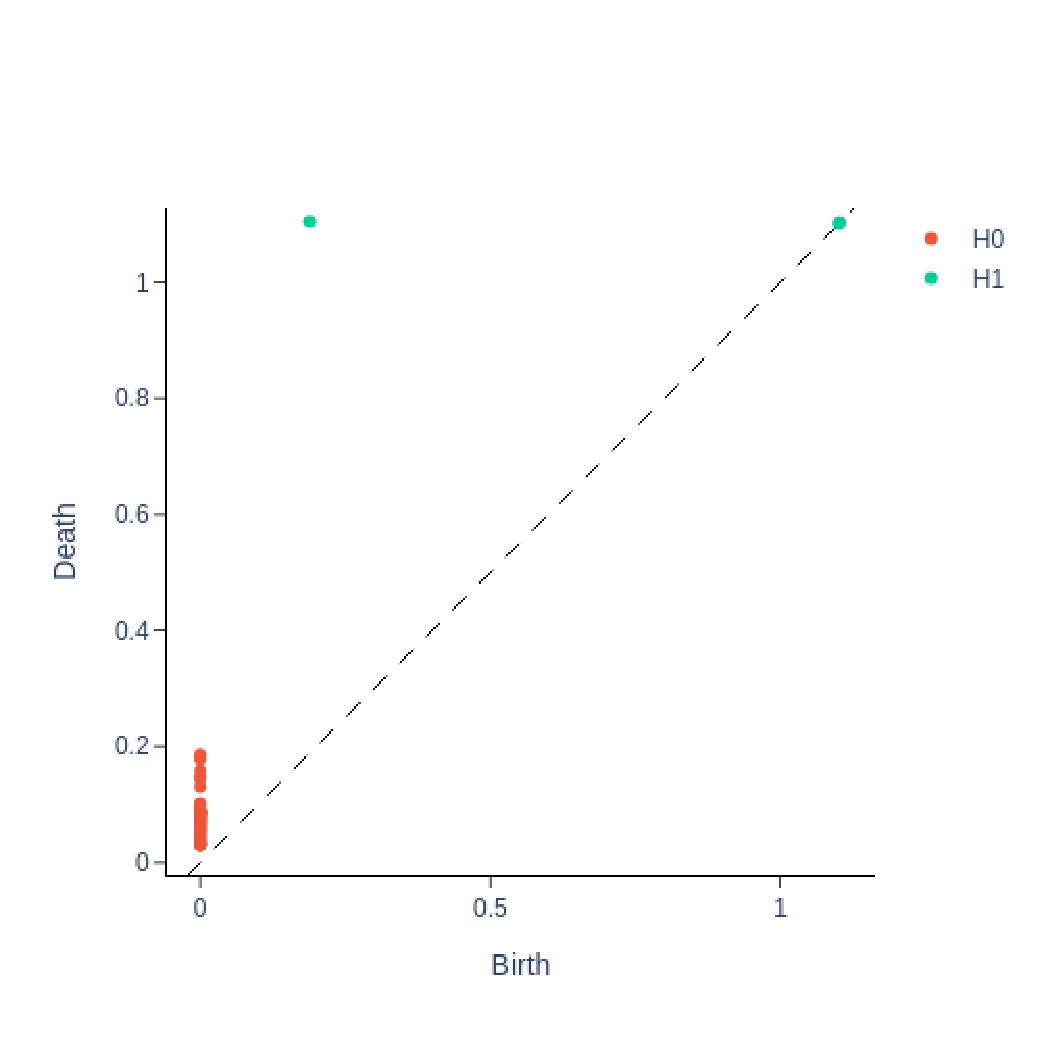
\includegraphics[width=7cm]{periodic_diagram.pdf} }}%
    \qquad
    \subfloat[\centering Diagram for the quasi-periodic wave]{{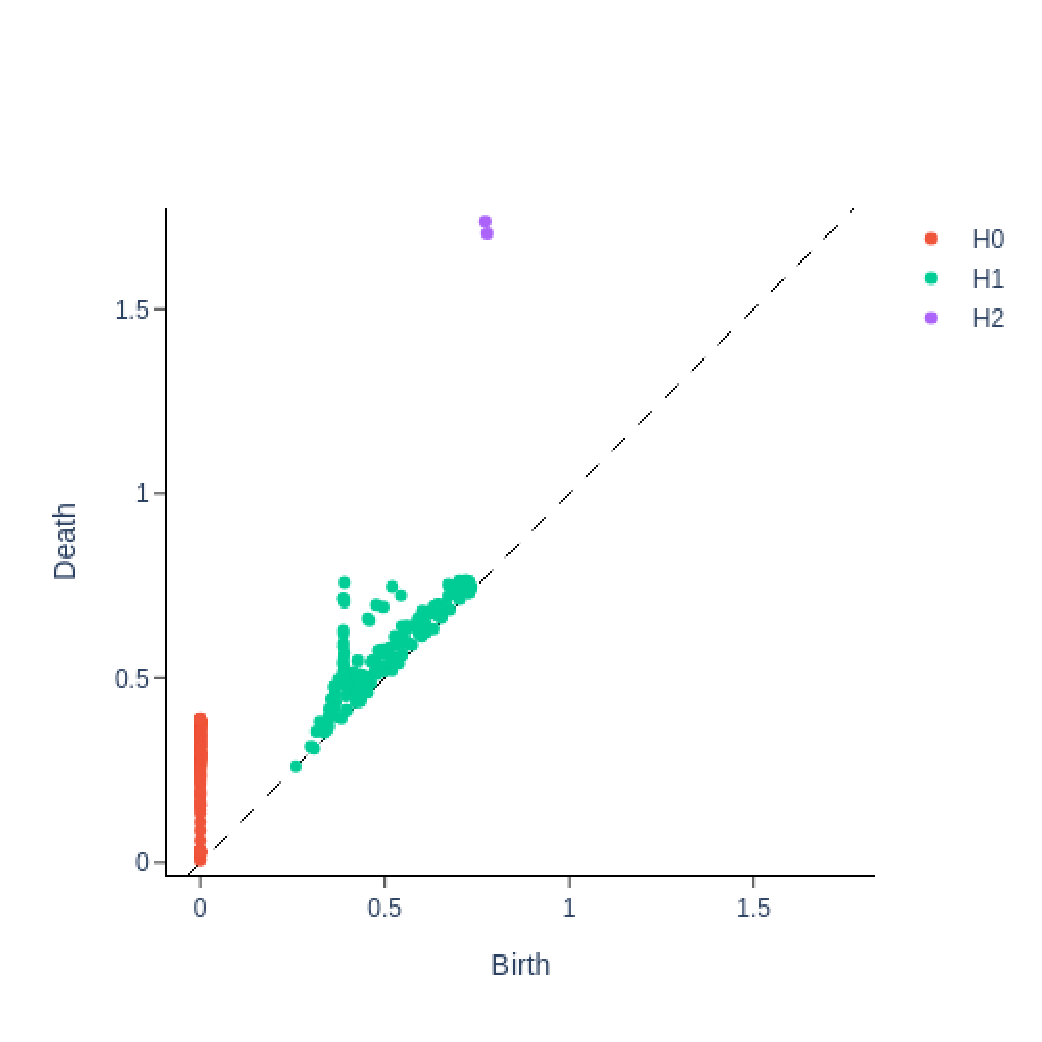
\includegraphics[width=7cm]{nonperiodic_diagram.pdf} }}%
    \caption{The corresponding persistence diagrams}%
    \label{fig:embedding_diagrams}%
\end{figure}

Instead of manually picking the values for the embedding, we can use the following two techniques to search for them automatically:
\begin{itemize}
  \item Mutual information for $\tau$
  \item False nearest neighbours for $\d$
\end{itemize}

To determine an optimal $\tau$, we first calculate the maximum $x_{\text{max}}$ and minimum $x_{\text{min}}$ values of the time series, dividing the interval between them into a large number of bins. Let $p_{k}$ be the probability that an element of the time series is in the $k$th bin and let $p_{j,k}$ be the probability that $x_{i}$ is in the $j$th bin while $x_{i+\tau}$ is in the $k$th bin. Then we define the mutual information as:

\begin{equation*}
  I(\tau) = -\sum_{j=1}^{n}\sum_{k=1}^{n}p_{j,k}(\tau)\log\left(\frac{p_{j,k}(\tau)}{p_{j}p_{k}}\right),
\end{equation*}
where $n$ is the number of bins on the interval $[x_{\text{min}}, x_{\text{max}}]$. The first minimum of this expression gives us the optimal time delay.

The false nearest neighbours algorithm assumes that points which are close in one embedding dimension should be close in a higher one. More precisely, if $p_{i}$ and $p_{j}$ are neighbours, we compute their normalised distance $R_{i}$ and check if is greater than some threshold $R_{\text{th}}$ in the next dimension:
\begin{equation*}
  R_{i} = \frac{|x_{i+m\tau}-x_{j+m\tau}|}{||p_{i}-p_{j}||} > R_{\text{th}}.
\end{equation*}
If this inequality holds, then we have a false nearest neighbour and we get the optimal embedding dimension $d$ by minimising the number of such neighbours.

We have to choose an upper bound for both $d$ and $\tau$ for the search to have a limit. We have chosen $d=30$ and a $\tau=30$ with a stride of 5. Once the search was finished, we have obtained optimal parameters $(d, \tau) = (6, 29)$. Due to the higher dimension, we used PCA to visualize the results in $\mathbb{R}^{3}$, as seen in \ref{fig:embedding_automatic}.

\begin{figure}[h!]
    \centering
    \subfloat[\centering For the periodic wave]{{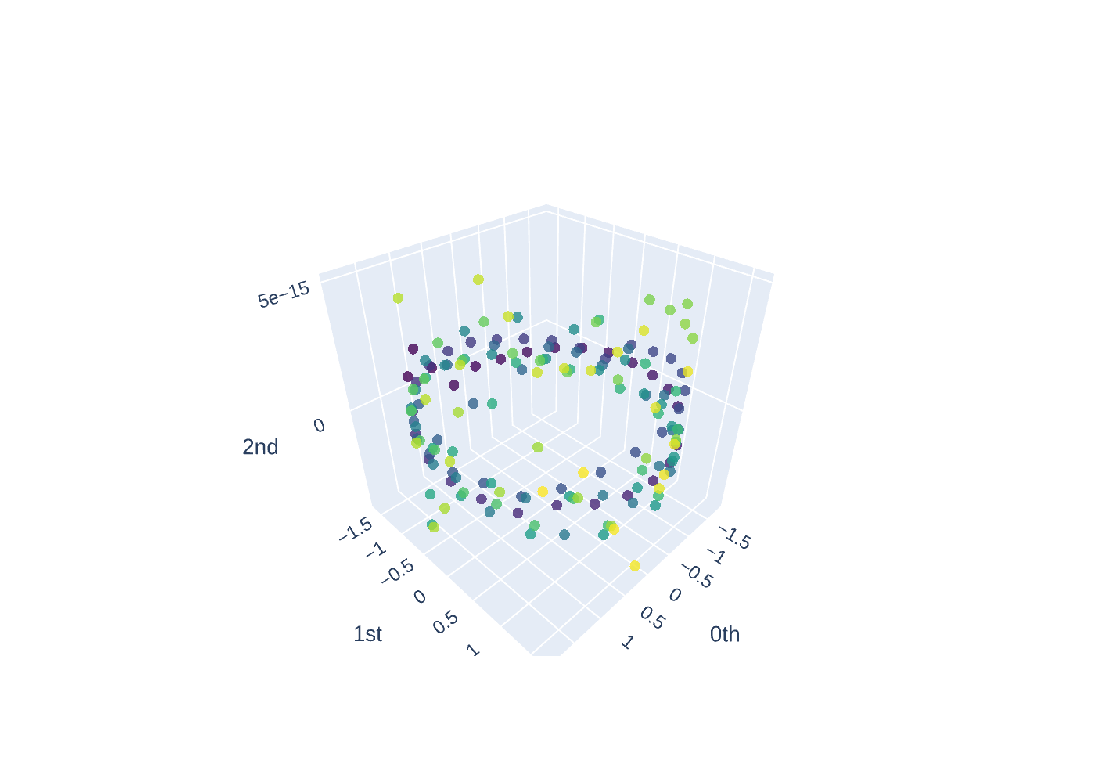
\includegraphics[width=7cm]{point_cloud_automatic1.pdf} }}%
    \qquad
    \subfloat[\centering For the quasi-periodic wave]{{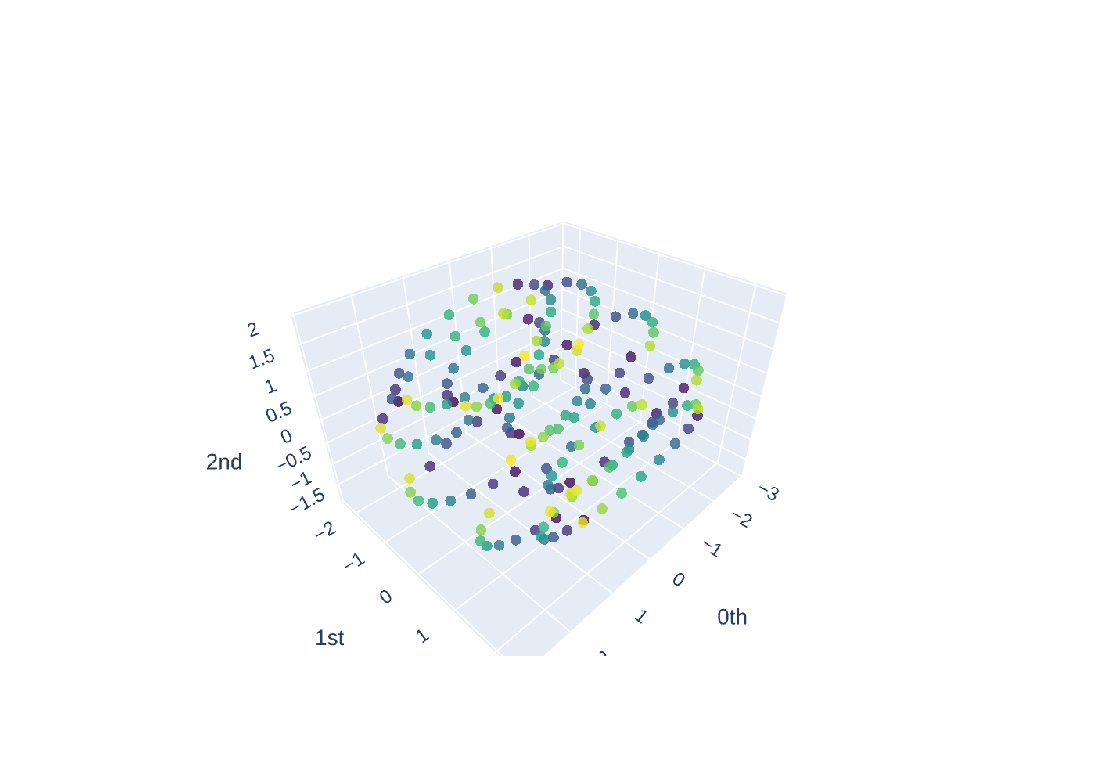
\includegraphics[width=7cm]{point_cloud_automatic2.pdf} }}%
    \caption{Optimal embeddings, after a reduction with PCA}%
    \label{fig:embedding_automatic}%
\end{figure}

Just as before, we can then compute their persistence diagrams, seen in \ref{fig:embedding_automatic_diagrams}. For the periodic signal, it is essentially the same. In the case of the quasi-periodic wave, there is less noise on the diagonal. Most importantly, we see two prominent $H_{1}$ points and one $H_{2}$ point, which corresponds to the signature of a hypertorus.

\begin{figure}[h!]
    \centering
    \subfloat[\centering For the periodic wave]{{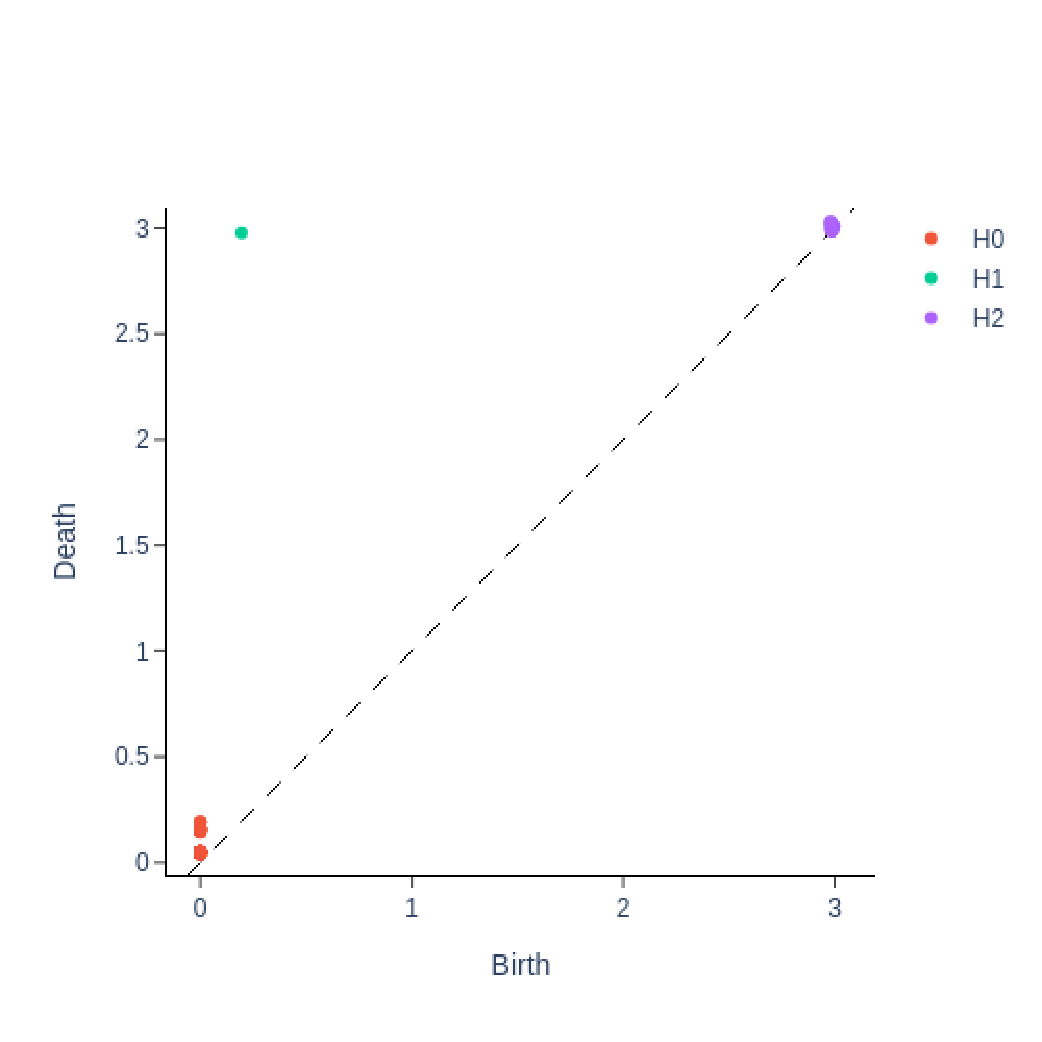
\includegraphics[width=7cm]{periodic_automatic_diagram.pdf} }}%
    \qquad
    \subfloat[\centering For the quasi-periodic wave]{{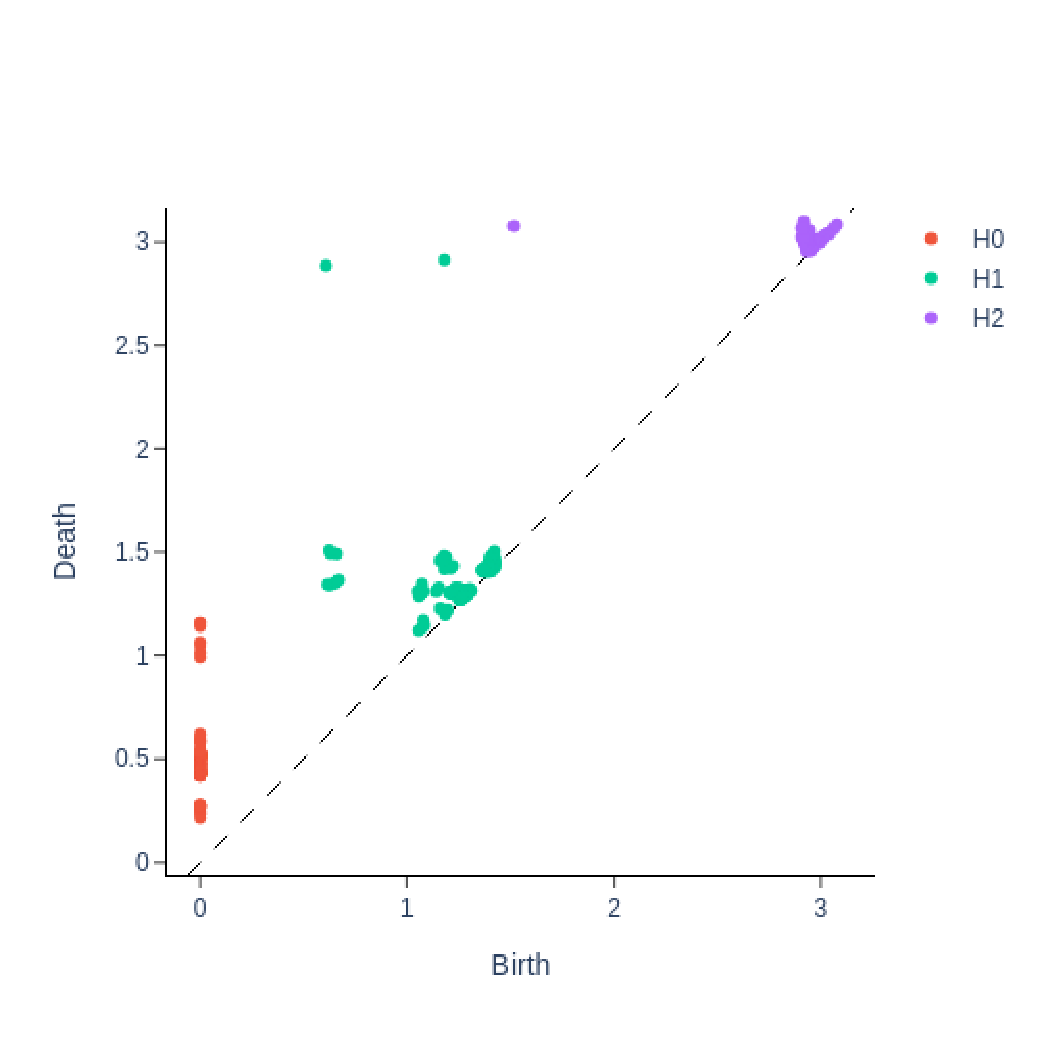
\includegraphics[width=7cm]{nonperiodic_automatic_diagram.pdf} }}%
    \caption{Persistence diagrams of the optimal embeddings}%
    \label{fig:embedding_automatic_diagrams}%
\end{figure}

Using sliding windows and Taken's embedding gives us tools to help us classify or cluster time series based on the topology of their embeddings. The notebook for the examples above can be found in \textit{src/Sliding Windows 1.ipynb}. In the notebook \textit{src/Sliding Windows 2.ipynb}, we provide further examples and simulations of sliding window embeddings, allowing the reader to play around with the parameters and see how the change in parameters affects the change in geometry and in the resulting persistence diagrams in a more interactive fashion. For example, we can see how the embedding is progressively more chaotic the more stochastic noise we add into the original signal, and how noisy the persistence diagram becomes in \ref{fig:embedding_noise}.

\begin{figure}[h!]
  \centering
  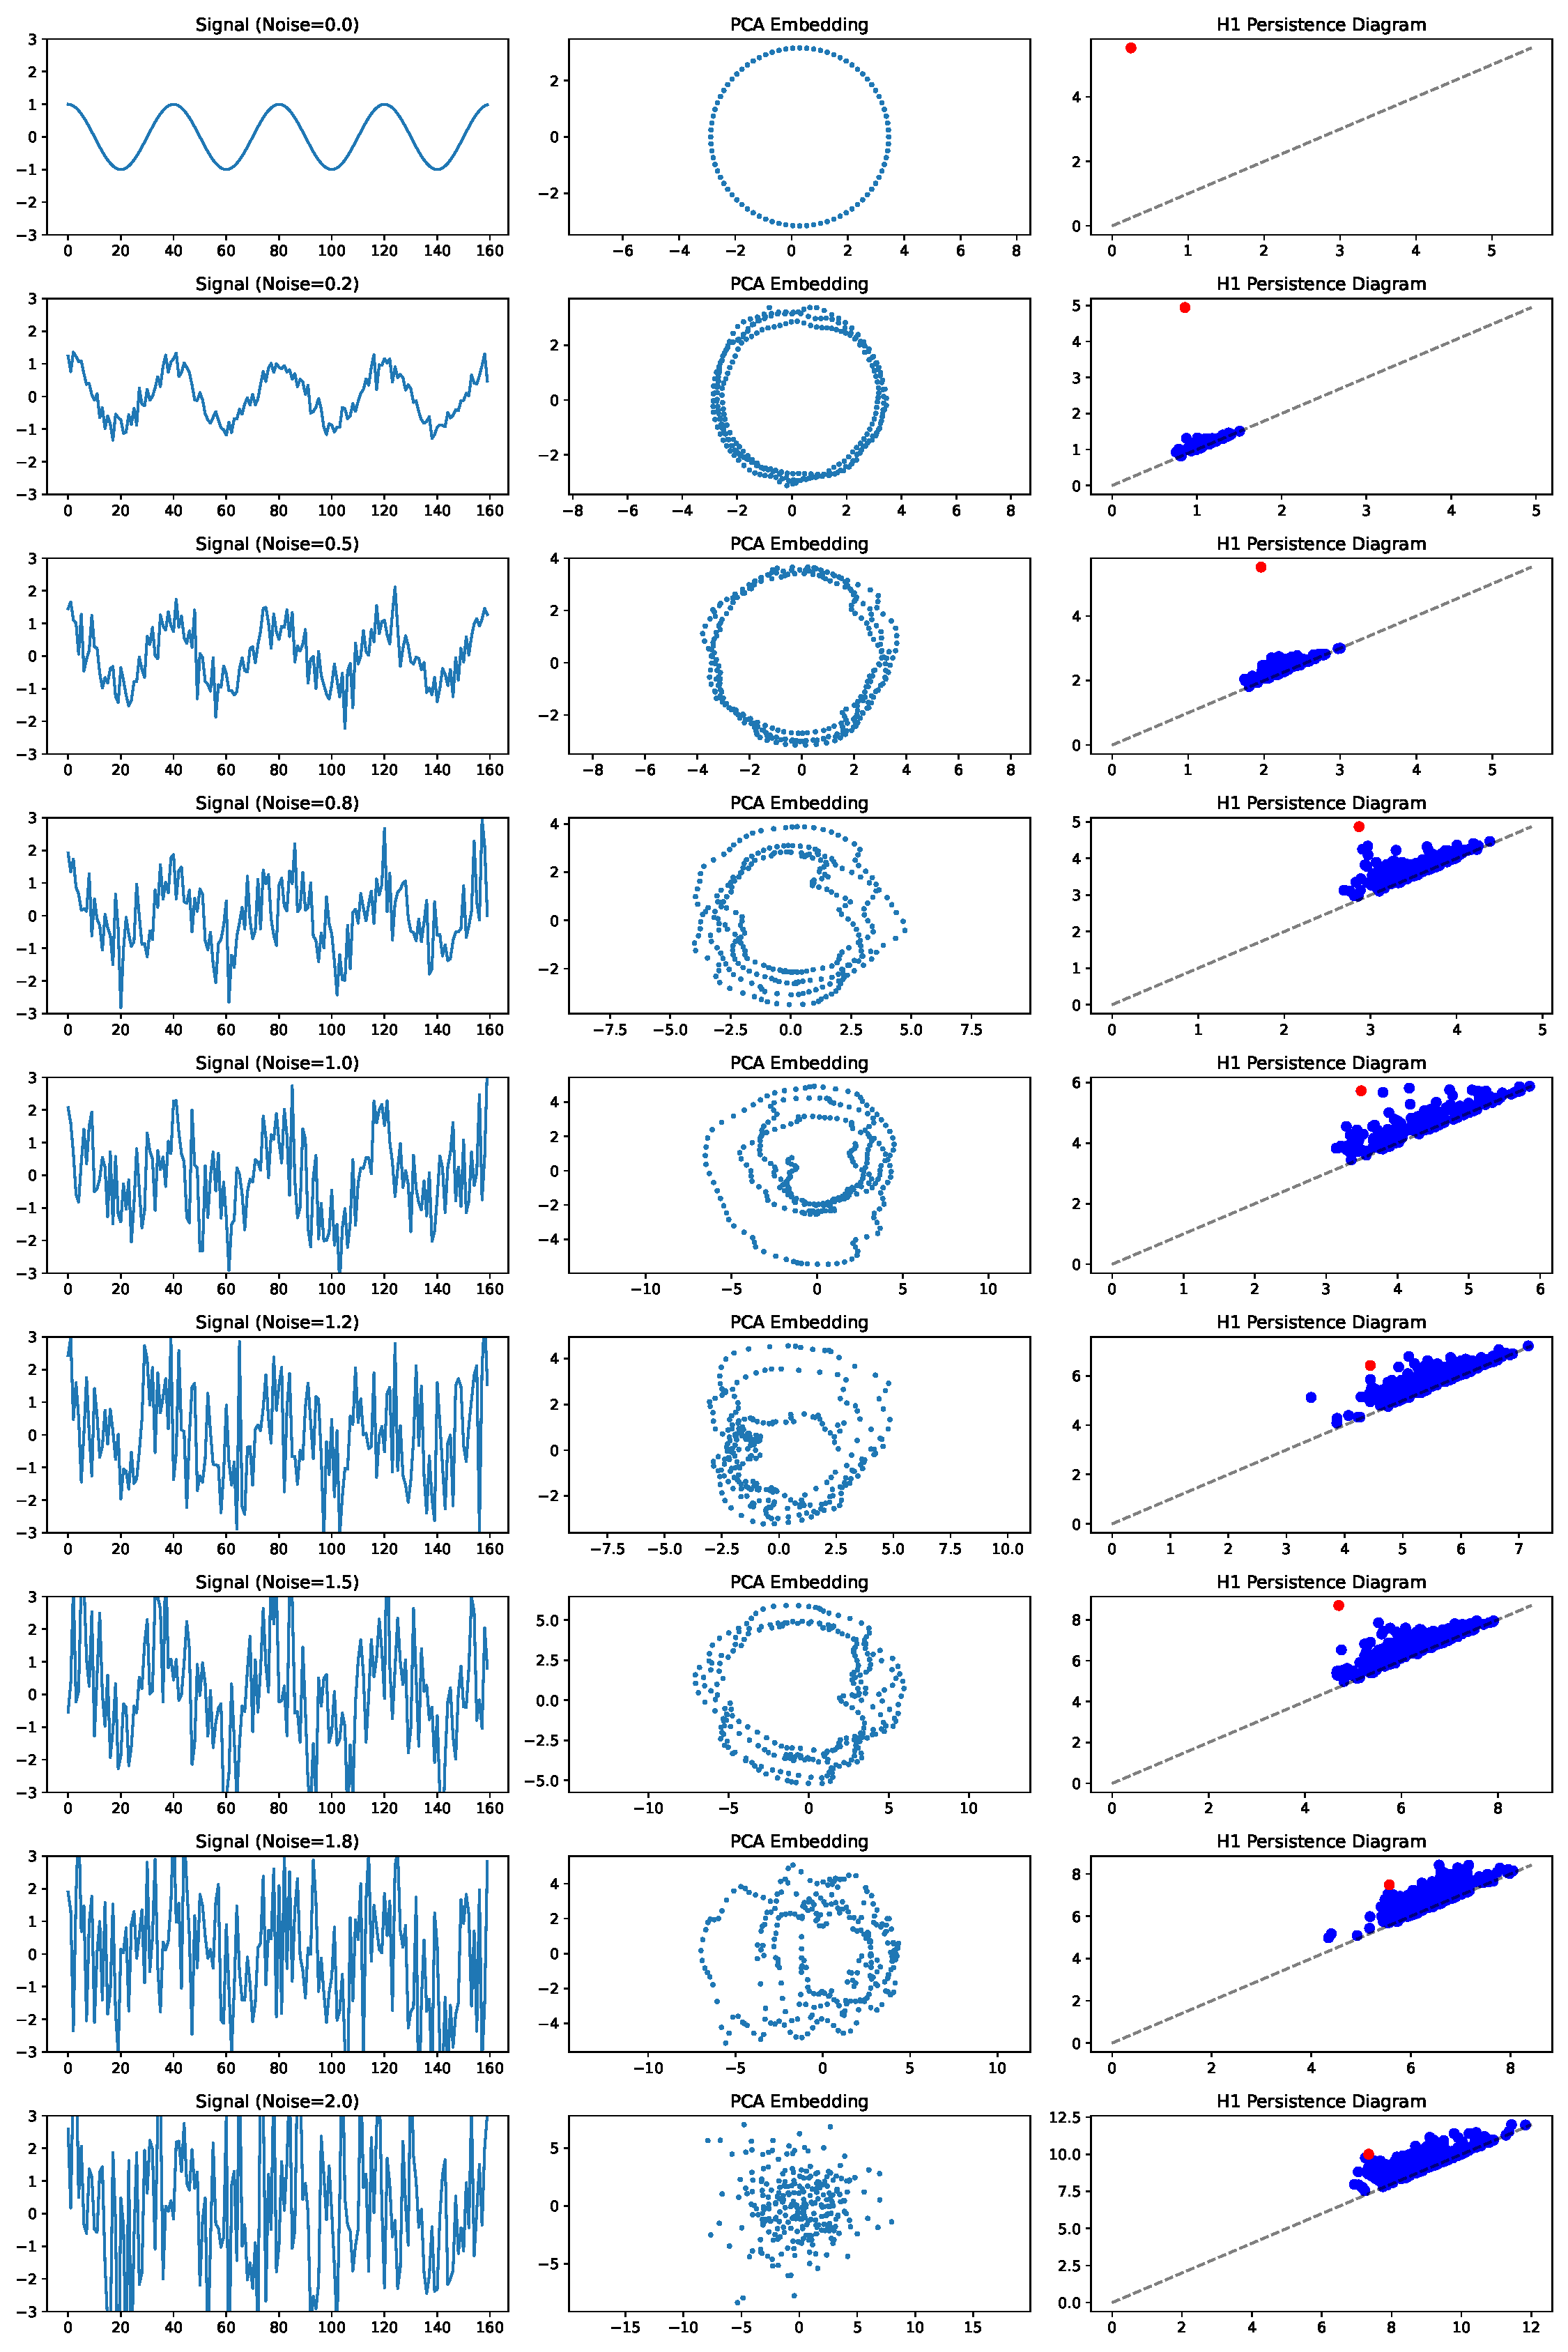
\includegraphics[width=15cm]{embedding_with_noise.pdf}
  \caption{The noisier our signal is, the less informative the geometry of its embedding and the persistence diagram becomes.}
  \label{fig:embedding_noise}
\end{figure}
